\documentclass[12pt,twoside]{article}
%\documentclass[11.75pt,twoside]{article}

 
\usepackage{float}
\usepackage[english]{babel}
\usepackage[utf8]{inputenc}
\usepackage{amsmath}
\usepackage{graphicx}
\usepackage{epsfig}
\usepackage[table]{xcolor}
\usepackage{multirow}
\usepackage[colorinlistoftodos]{todonotes}
\usepackage[hidelinks]{hyperref}
\usepackage[a4paper,hmargin=2cm,vmargin=0.6cm,includeheadfoot]{geometry}
\usepackage[font=footnotesize]{caption}
\usepackage{natbib}
%\bibliographystyle{ieeetr}
\bibliographystyle{abbrvnat}
\setcitestyle{authoryear,open={(},close={)}} %Citation-related commands

\usepackage[font={footnotesize}]{caption}

\usepackage{authblk}

\usepackage{times}
%\usepackage{arial}

\usepackage{wrapfig}

\usepackage[export]{adjustbox}


% line numbers
\usepackage[right]{lineno} % JG_ADD
\linenumbers
\modulolinenumbers[1]

\raggedbottom 
\linespread{1.25} 

\title{A comprehensive investigation of intracortical and corticothalamic models of the alpha rhythm}

\author[1,2]{Sorenza P. Bastiaens}
\author[2,3]{Davide Momi}
\author[1,2,4]{John D. Griffiths}
\affil[1]{Institute of Medical Sciences, University of Toronto}
\affil[2]{Krembil Centre for Neuroinformatics, Centre for Addiction and Mental Health, Toronto}
\affil[3]{Department of Psychiatry and Behavioral Sciences, Stanford University Medical Center, Stanford, California}
\affil[4]{Department of Psychiatry, University of Toronto}


\date{}%March 2024}

\begin{document}
\maketitle

%\headheight={11pt}

%TC:ignore
\begin{abstract}
The electroencephalographic alpha rhythm is one of the most robustly observed and widely studied empirical phenomena in all of neuroscience.  However, despite its extensive implication in a wide range of cognitive processes and clinical pathologies, the mechanisms underlying alpha generation in neural circuits remain poorly understood. 
In this paper we offer a renewed foundation for research on this question, by undertaking a systematic comparison and synthesis of the most prominent theoretical models of alpha rhythmogenesis in the published literature. We focus on four models, each studied intensively by multiple authors over the past three decades: i) Jansen-Rit, ii) Moran-David-Friston, iii) Robinson-Rennie-Wright, and iv) Liley-Wright. Several common elements are identified, such as the use of second-order differential equations and sigmoidal potential-to-rate operators to represent population-level neural activity. Major differences are seen in other features such as wiring topologies and conduction delays. Through a series of mathematical analyses and numerical simulations, we nevertheless demonstrate that the selected models can be meaningfully compared, by associating parameters and circuit motifs of analogous biological significance.
With this established, we conduct explorations of rate constant and synaptic connectivity parameter spaces, with the aim of identifying common patterns in key behaviours, such as the role of excitatory-inhibitory interactions in the generation of oscillations. Finally, using linear stability analysis we identify two qualitatively different alpha-generating dynamical regimes across the models: i) noise-driven fluctuations, and ii) self-sustained limit-cycle oscillations, emerging due to an Andronov-Hopf bifurcation. The comprehensive survey and synthesis developed here can, we suggest, be used to help guide future theoretical and experimental work aimed at disambiguating these and other candidate theories of alpha rhythmogenesis.

\end{abstract}
%TC:endignore
\newpage
\tableofcontents


%- Technically oriented summary; 
%- Alpha rhythms are important
%- We review the most prominent mathematical models of alpha rhythm activity in terms of their wiring topology, dynamics, linearized forms, parameterization, and biological interpretation. 
%- The models are x,y,z 
%- They have common elements (sigmoid, impulse response). 
%- They differ in terms of blah 
%- We make that unified parameter table across models
%- Correspondences across models are found / studied in terms of E/I loops etc and their effects on linearized system stability and dynamical regimes
%- This is useful because x 


\newpage
%TC:ignore
\section{Background}
\subsection{Overview and aims}
%TC:endignore
The classical alpha rhythm is an approximately 8-12Hz oscillatory activity pattern that is highly prominent in electroencephalogram (EEG), electrocorticogram (ECoG), and local field potential (LFP) recordings from humans and other species, particularly during states of quiet wakefulness (Fig. 1A). Almost 100 years after its discovery \citep{berger1929elektroenkephalogramm}, alpha frequency activity remains one of the most robustly observed and broadly significant phenomena in all of neuroscience, yet also one of the most enigmatic \citep{bollimunta2011neuronal}. Alpha plays a fundamental role in a wide range of cognitive processes, and abnormal alpha rhythms are frequently identified in psychiatric and neurological conditions (\citealp{bucci2004executive, clancy2017restless,deiber2020linking,jensen2010shaping}; summarized in Fig. 1A, panel 3). However, despite the profound importance of alpha rhythms - both in terms of their undeniable prominence in empirical EEG data, and their implication across a broad range of phenomena across clinical and cognitive neuroscience, their mechanistic physiological basis and functional significance remains unclear. Several theories of alpha rhythmogenesis have been proposed over the years, often emphasizing different physiological substrates such as pacemakers, recurrent activity and excitatory-inhibitory interactions in cortical column microcircuits, or delayed inhibitory feedback within cortico-thalamocortical loops (Fig. 1B). There have however been relatively few attempts to evaluate and compare in detail these alternative theories in conjunction, and thereby arrive at a useful synthesis of the most compelling accounts. Developing such a synthesis is a principal aim of the present study. 

A central criterion around which we base this investigation is the requirement that the models of interest should be expressed in concrete mathematical language, as well as being implemented in numerical simulations and/or quantitative analytic computations. Specifically, we consider a particular class of neurophysiological model - neural population models (NPMs) - that amongst the different mathematical formulations used over the past half century of efforts to model and understand alpha activity (Fig. 1C) are the one that has been used most routinely  \citep{da1977cortical,grimbert2006bifurcation,jansen1995electroencephalogram,liley2001spatially,bhattacharya2011thalamo,david2003neural,hartoyo2019parameter,robinson2003neurophysical}. 
%By analyzing and comparing the implicated circuits in terms of their dynamics, topologies, and parameters, we are able to extract further mechanistic insights into these principal models and theories of alpha rhythmogenesis. 
We focus on four extensively studied NPMs that are commonly used to describe EEG alpha activity in the neuroimaging, neurophysiology, and computational neuroscience literature: the Jansen-Rit (JR; \citealt{jansen1995electroencephalogram}), Moran-David-Friston (MDF; \citealt{david2003neural, moran2007neural}), Liley-Wright (LW;  \citealt{liley1999continuum, liley2001spatially}), and Robinson-Rennie-Wright (RRW; \citealt{robinson2002dynamics, robinson2003neurophysical}) models. These shorthand terms reference certain key individuals who contributed to the conception and/or development of several prominent strands in the research literature. We do note however that they are imperfect ones - both because all of the models studied here build directly on the earlier work of other important theoreticians (e.g. Freeman, Zetterberg, Lopes Da Silva, Cowan, Nunez), and also in some cases each other (e.g. MDF is an indirect extension of JR). 
We begin over the next few sections with a description of general elements present in the JR, MDF, LW, and RRW models, and a summary of their individual  characteristics. Direct comparisons between each of them are then made, first in the context of the alpha regime, and then extending into other oscillatory regimes at non-alpha frequencies.
A central objective in this work is to identify common patterns between the models, using numerical simulations across a broad parameter space to identify the effects of rate constants, inter-population connectivity structure, and other factors on oscillatory dynamics. These similarities and differences across models constitute the points of agreement and divergence across current theories of alpha rhythmogenesis, and it is the mapping of this theoretical landscape that is our main aim in the present paper. The origin, biological significance, and validity of their parameters, as well as the functional forms of their equations, are also considered when discussing the respective limitations and advantages of each candidate model. 

\subsection{Alpha origins and rhythmogenesis: current theories}

%TC:ignore
%\vspace{-1cm}
%\begin{wrapfigure}{r}{0.75\textwidth}
\begin{figure}[H]
    \centering
    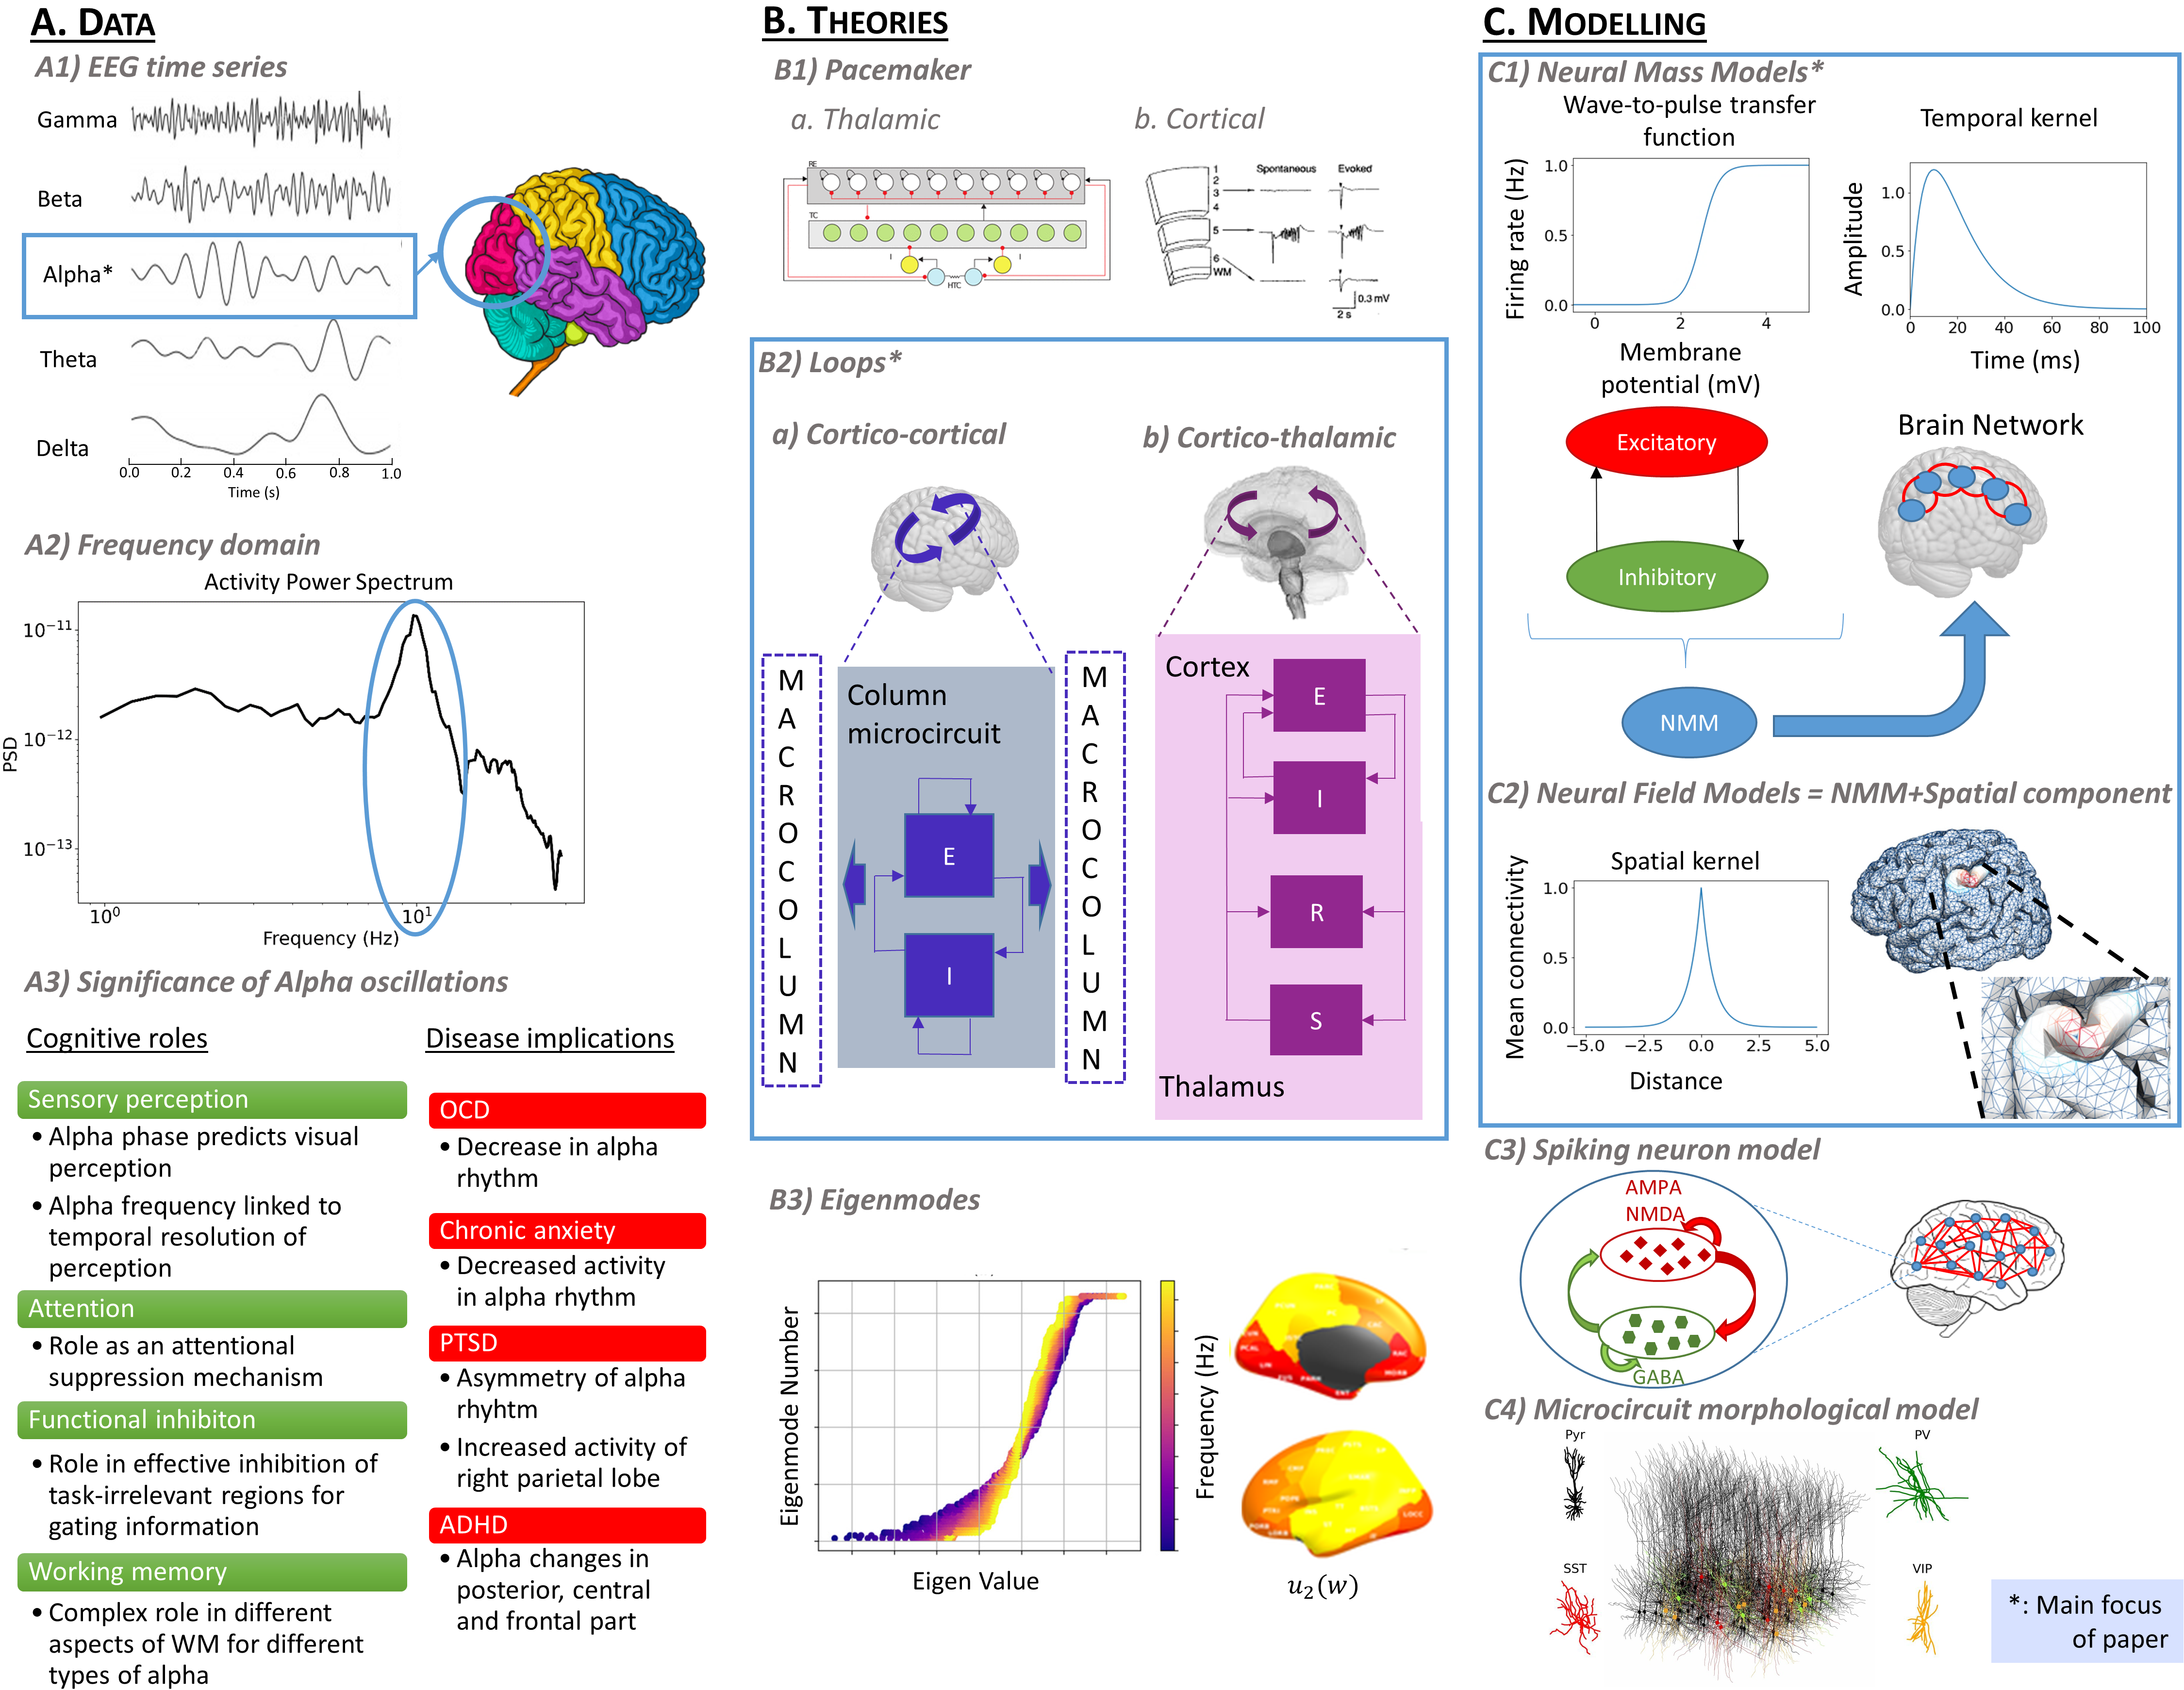
\includegraphics[scale = 0.4]{Images/Fig1__Overview_final.png} %[width=0.75\textwidth,right]{Images/Fig1__Overview_final.png}
    \caption*{\textbf{Figure 1. \textit{Data, theories, and models of the EEG alpha rhythm.}} \textbf{A)} Alpha oscillations are most strongly observable in the occipital lobe of the cerebral cortex (A1), where they are characterized by a peak in the power spectrum between 8-12Hz (A2). Panel A3 summarizes the role alpha plays in cognitive processes, as well as abnormal alpha rhythm features observed in various diseases (see refs in main text). \textbf{B)} Summary of the different theories that have been proposed to explain the alpha rhythm. We focus on theories emphasizing the importance of interactions between neural populations (B2). \textbf{C)} Alpha rhythm theories are clarified and concretized by mathematical formulations, allowing numerical and analytical investigation of their predictive and explanatory scope. The principal class of models used to date are neural population (neural mass and neural field) models (C1 and C2), which are the focus of the present work.}
    \label{fig:Overview}
\end{figure}
\vspace{-0.5cm}
%\end{wrapfigure}
%TC:endignore
%\section{Background} if possible replace intro with background
Neural oscillations are repetitive, quasiperiodic patterns of brain activity that are believed to play a key role in various sensory-cognitive processes \citep{pmid24174901}. In humans, oscillations are most commonly captured with EEG, a non-invasive neuroimaging modality that uses scalp-recording electrodes to capture large-scale neuroelectric activity with high temporal resolution. 
%EEGs measure differences in electrical potential between recording and reference electrodes on the scalp that results from summed postsynaptic dipoles in the brain. 
In order to quantify oscillatory activity, the measured signal is typically decomposed into its power spectrum frequency components via a Fourier or related transform, and subsequently often aggregated into several canonical frequency bands. %(delta: 1-4Hz, theta: 4-8Hz, alpha: 8-12Hz, beta: 12-35Hz, gamma: above 35Hz) for further analysis \citep{ABHANG201619}.
%(maybe finish on alpha theories as well? Or like how can use models to further explore alpha origin? Outline has changed a bit since need to make sure it corresponds) \\
Alpha-frequency oscillations, or `alpha waves', usually defined as the EEG frequency band between 8 and 12 Hz \citep{MOINI2020177}, are associated with quiet wakefulness, meditation, relaxation and reflection \citep{halgren2019generation}. In EEG recordings, alpha waves are most prominent around the occipital lobe when the subject is awake with eyes closed and not engaged in a stimulus-locked cognitive task, also known as the \textit{resting state} \citep{klimesch1999eeg}. Their role is believed to be fundamental for a number of top-down cognitive processes \citep{halgren2019generation} such as sensory perception \citep{samaha2015speed}, attention (as an attentional suppression mechanism -  \citealt{foxe2011role}), functional inhibition \citep{jensen2010shaping}, working memory \citep{wianda2019roles} and long-term memory \citep{klimesch2012alpha}.
Abnormal EEG rhythmic patterns, including aberrant alpha oscillations, are indicative of atypical bioelectrical activity that may suggest the presence of cognitive and/or mental disorders \citep{scally2018resting, buchanan2021elevated, abela2019slower, fingelkurts2006composition, roohi2017changes, metzger2004ptsd, roohi2017changes}. %Thus, robust resting state alpha activity is considered an indicator of healthy cognitive functioning. Reduced alpha power or lowered alpha peak frequencies resulting from aging, head trauma, or exposure to toxins may be correlated with a neurological disorder or brain impairment, such as traumatic brain injury (TBI), or dementia \citep{scally2018resting, buchanan2021elevated}. Both the power and topography of the alpha rhythm is altered in epilepsy patients \citep{abela2019slower}. Several psychiatric conditions are also associated with a decrease in activity in the alpha rhythm, namely chronic anxiety \citep{fingelkurts2006composition, roohi2017changes}, and obsessive compulsive disorder (OCD), sometimes accompanied by concomitant changes at theta and beta frequencies \citep{karadag2003quantitative}. Asymmetry of the alpha rhythm and increased activity of the right parietal lobe is observed in patients experiencing post-traumatic stress disorder (PTSD) \citep{metzger2004ptsd,roohi2017changes}. 
A comprehensive survey of the vast research literature on alpha in cognitive and clinical neuroscience is beyond the scope of the present work; for this we refer the reader to excellent recent treatments by \citet{ippolito2022role} and \citet{bacsar2012short}.

%Even though it was the first rhythmic wave documented and named by Hans Berger in 1929 \citep{berger1929elektroenkephalogramm, tudor2005hans}, and is considered the predominant oscillation in the human brain \citep{klimesch2012alpha} of great importance in terms of their prominence in empirical EEG data, and their implication across a number of clinical and cognitive neuroscience as illustrated previously - the physiological mechanism behind their generation as well as their functional significance remains elusive. 
Although the alpha rhythm was the first rhythmic wave identified and named by Hans Berger in 1929 \citep{berger1929elektroenkephalogramm, tudor2005hans}, and is considered the predominant oscillation in the human brain \citep{klimesch2012alpha} with significant implications in empirical EEG data and various clinical and cognitive neuroscience studies, the physiological mechanisms underlying its generation and functional significance remain poorly understood.
%The complexity is in part due to the likely existence of multiple independent alpha-generating circuits supported by both thalamo-cortical and cortical-cortical loops, since self-sustaining sources have been identified in both regions (layer V of the cortex and thalamus) \citep{nakagawa2014delays}.
%The complexity arises from the probable presence of multiple independent circuits generating alpha waves, which are supported by thalamo-cortical and cortical-cortical loops. Self-sustaining sources have been identified in both regions, namely the thalamus and layer V of the cortex \citep{nakagawa2014delays}. 
Unlike other well-characterized brain oscillations, such as beta and gamma waves, whose neural circuitry is believed to rely on local connectivity alone \citep{lozano2018physiological}, the generation of alpha rhythm has been proposed to involve contributions from both cortical and thalamic brain regions, which may also influence and interfere with each other \citep{lozano2018physiological,da1991neural}. Several hypotheses have been proposed regarding the composition and mechanistic organization of these alpha circuits, which can be grouped under three categories: \textit{pacemaker}, \textit{local network}, and \textit{global network} theories. A thorough review of the pacemaker and global network theories are beyond the scope of the present review, but some additional notes and references are provided in Fig. 1 and S.10, and an extensive discussion can also be found in \cite{nunez2006electric}. Local network theories propose that alpha rhythms are produced by interactions between excitatory and inhibitory neural populations, typically equipped with dendritic response function terms and saturating nonlinearities \citep{valdes2010white}. This theory class is by far the most established and extensively studied of the three, and therefore serve as the primary focus of the present paper. Specifically, we examine in detail the two prevailing variants of the local network theory of alpha rhythmogenesis, whose central tenets are the following: 

\begin{enumerate}

\item   \textbf{Intracortical theory}: Alpha oscillations are generated by recurrent activity and excitatory-inhibitory interactions within cortical column microcircuits.%[source]

\item	\textbf{Corticothalamic theory}: Alpha oscillations are generated by delayed inhibitory feedback within corticothalamocortical loops.   %[source]

%\item   The harmonic eigenmode structure of large-scale cortico-cortical networks is a core determinant of the 8-13Hz characteristic frequency range.% [source]

%\item   Thalamic and cortical pacemaker neurons are responsible for the generation of the alpha waves. %[source]

\end{enumerate}

These two accounts describe the origin of alpha waves as a phenomenon relying on dynamics of local networks of interconnected neural populations, and thus occurring at the \textit{mesoscopic} spatial scale. Computations underlying brain functions such as action, perception, learning, language and higher cognition have been hypothesized to also originate from activity within neural ensembles at this spatial scale \citep{deco2008dynamic}. However, whilst current neural recording technologies allow straightforward measurement of macroscale (EEG, MEG, fMRI, ECoG) or microscale (single cell recording, fluorescence calcium imaging, multielectrode arrays) activity, mesoscopic activity is more challenging to measure directly. To help bridge the gap between these scales, and explore the rhythmogenic mechanisms entailed by the two local theory types summarized above, mathematical models implementing these theories have largely focused on describing and simulating mesoscale neural population wiring and activity. 

%stronger transition
%TC:ignore
\begin{figure}[H]
    \centering
    %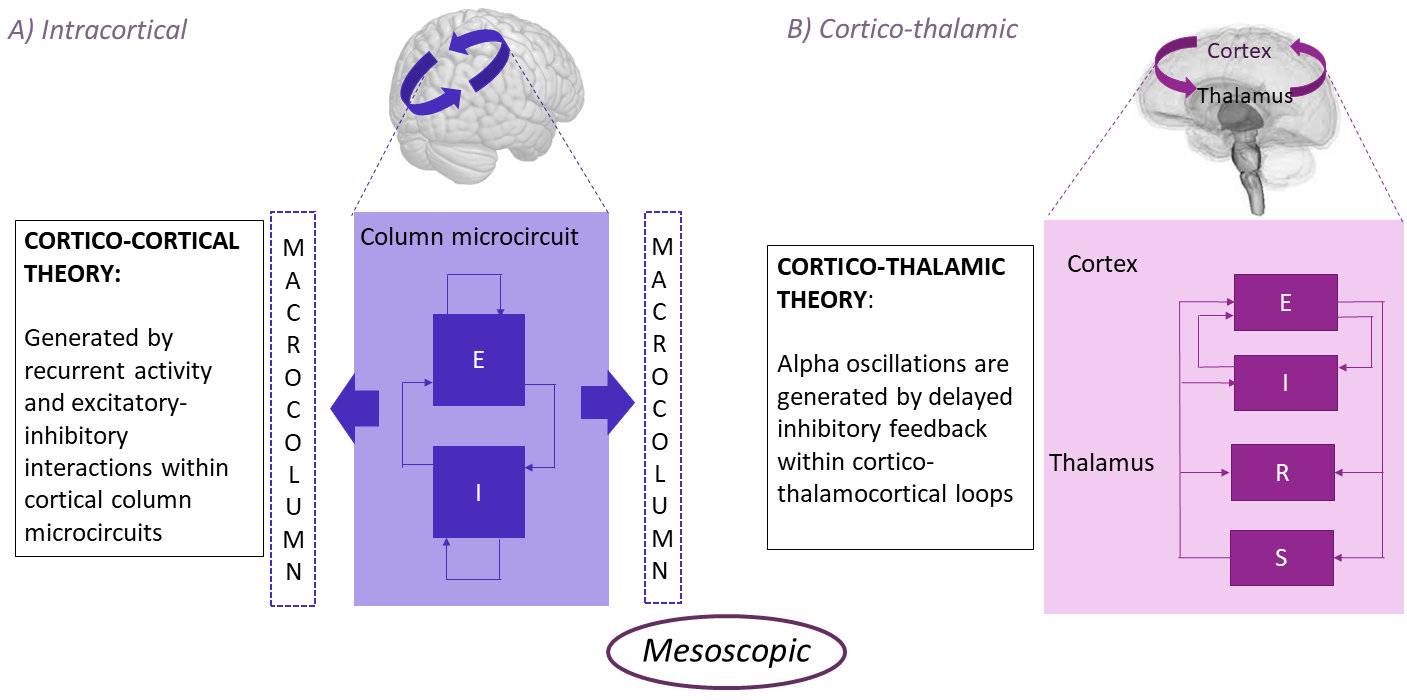
\includegraphics[scale=0.45]{Images/Figure2_theories.png}
    %\caption*{\textbf{Figure 2.  \textit{ Schematic depiction of the two main theories focused on local neural population connectivity to explain alpha rhythmogenesis from which mathematical models are built.}} \textbf{A)} Cortico-cortical model which consists of interconnected macrocolumns each composed of excitatory and inhibitory neural populations. \textbf{B)} Cortico-thalamic model which includes neural populations of the thalamus in the process of alpha genesis.}
    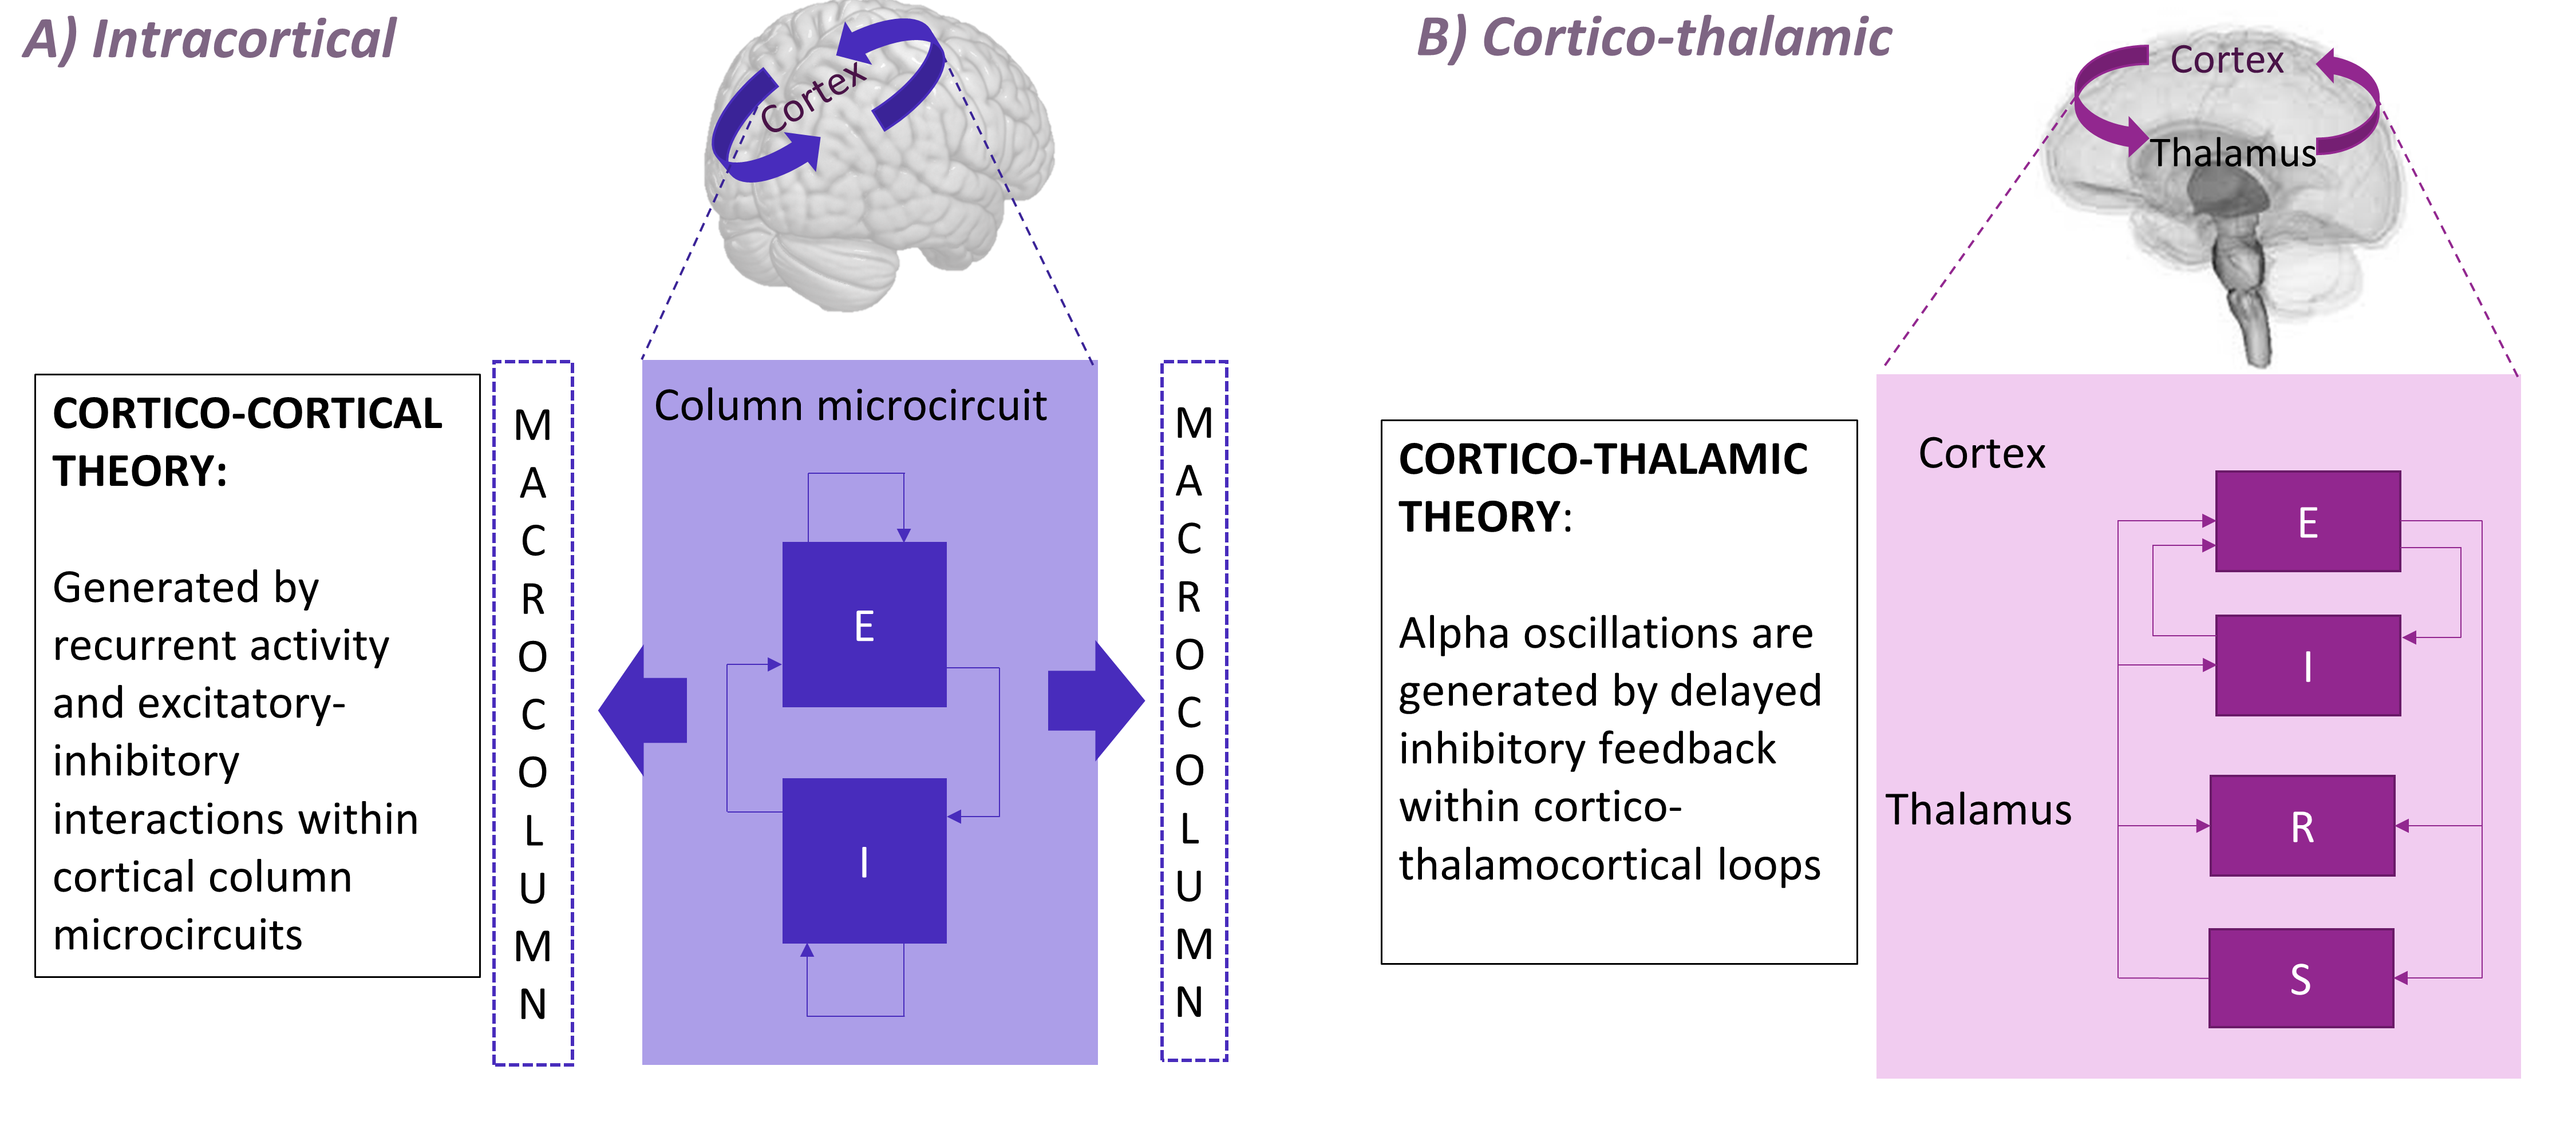
\includegraphics[scale=0.45]{Images/Fig2__Theories.png}
    \caption*{\textbf{Figure 2. \textit{Schematic depiction of two candidate theories of alpha rhythmogenesis.}} \textbf{A)} Cortico-cortical columnar microcircuit model, representing the generation of alpha rhythm through interconnected macrocolumns. \textbf{B)} Cortico-thalamic model, involving thalamic neural populations in the process of alpha genesis.}
    \label{fig:Theories}
\end{figure}
\vspace{-\baselineskip} 
%\subsection{Mathematical models of neural population dynamics}
\subsection{Bridging scales: mathematical modelling of mesoscopic neural population dynamics}
%TC:endignore

Mathematical models of human brain activity have provided significant insights into neural processes at multiple scales \citep{deco2008dynamic}. The present study focuses on the alpha rhythm using a `top-down' approach, whereby a mathematical expression is used that represents the collective activity of neuron groups rather than individual cells \citep{cook2021neural, cooray2023global}. A general term for this set of techniques is neural ensemble or \textit{neural population models} (NPMs). NPMs consider the aggregate activity of neuron populations with common synaptic connectivity (excitatory or inhibitory), assuming uncorrelated states across the ensemble, and capturing emergent properties of neural tissue patches \citep{breakspear2017dynamic}. This method is effective for modelling oscillatory activity like the alpha rhythm, aligning with the spatial scales of EEG channels and approximating local field potentials \citep{coombes2014neural, evertz2022alpha}. 

NPMs include neural mass models (NMMs), mean-field models (MFMs), and neural field models (NFMs; \citealp{deco2008dynamic, bojak2014neural}) - however it should be noted that the terminology for these NPM sub-types is not used consistently across the published literature. In one prominent strand of work \citep{deco2008dynamic, moran2013neural} the term `MFM' is reserved specifically for NPMs that simplify neural population activity using a diffusion approximation, defining it as a standard normal probability distribution characterized by the mean and variance of the firing rate, with stochastic dynamics governed by Fokker-Planck equations. In this schema, NMMs are defined as a specific type of NPM where the variance of the state variables (e.g. average firing rate) across the population is fixed, allowing a simpler representation of the dynamics than MFMs with fewer equations \citep{breakspear2017dynamic}. NMMs are `point process' models, i.e. they describe neural population activity without any explicit spatial information. In contrast, NFMs include local spatial information by considering the cortex as a smooth and continuously connected sheet, supporting phenomena such as propagating activity waves, often described by damped wave equations \citep{pinotsis2014neural, breakspear2017dynamic}. Both NMMs and NFMs can be used to simulate whole-brain activity, by coupling local neural populations according to a discrete weighted connectivity matrix (`anatomical connectome'), or a continuous cortical surface manifold, respectively \citep{breakspear2017dynamic, schirner2018inferring, glomb2021computational, robinson2016eigenmodes, nunez2006electric, visser2017standing}. For a detailed review of NPM development and whole-brain modelling, see \citet{griffiths2022whole} and \citet{chow2020before}, and additional remarks given in S.10. 

% JG: ACTUALLY I THINK THIS PARA IS NOT NEEDED 
%Within the literature on NPM-based simulations of EEG alpha rhythms, there are four models that stand out as being the most extensively studied - both in terms of published articles and numerical+mathematical exposition. These are the JR, MDF, LW, and RRW models introduced in Section 1.1. Before beginning our detailed analysis and evaluation of these four models, we first conclude our background review in the next section with a discussion of the two central mathematical components of these and most other NPMs.


%TC:ignore
\subsection{Classification of NPMs and mathematical characteristics of \\ convolution-based models}
%TC:endignore
The three NPM variants discussed above represent three different approaches to the treatment of heterogeneity in mesoscale activity patterns - with NFMs describing variation over space, MFMs describing variation within a point process as a statistical distribution, and NMMs simplifying both of these by assuming no spatial or statistical variation. NPMs can also be categorized according to their general approach to the mathematical description of neural population-level activity, with the main distinctions being convolution vs. conductance-based and voltage vs. activity-based models. Activity-based models, such as the Wilson-Cowan equations \citep{wilson1972excitatory,cowan2016wilson} have state variables representing the proportion of active cells in the population, while voltage-based models represent the population-average membrane potential within various neuron classes. Conductance-based NPMs assume very high coherence between neurons, to the extent that the dynamics of neuron population resembles the dynamics of each single neuron, allowing the use of equations that follow the same structure as single neuron conductance-based models \citep{marreiros2010dynamic,breakspear2017dynamic}, with distinct ionic current types and corresponding channel kinetics. We refer the reader to \citet{marreiros2010dynamic, pinotsis2013conductance, moran2011vivo, moran2013neural} for further discussion on the nuances of conductance-based and activity-based modelling approaches, and restrict the remainder of our discussion here to convolutional voltage-based NPM type, of which the four models focused on in this paper are all variants.

%For conductance-based models, very high coherence between neurons is assumed, to the extent that the dynamics of neuron population resembles the dynamics of each single neuron. The mathematical equations then follow the same structure as single neuron conductance-based models \citep{marreiros2010dynamic,breakspear2017dynamic}. Since distinct types of ionic currents are explicitly modelled, a direct relationship between modelled synaptic processes and physiological mechanisms can be determined \citep{moran2011vivo}. 

%The four models reviewed in this paper are considered convolution-based models, each with slightly different expressions or additional elements. They rely on empirical observations of the collective response of a neural population to their inputs, to build a phenomenological model that captures the system's response. Although convolution-based models lack the biological detail of conductance-based models, they provide a more straightforward and interpretable framework for understanding the system-level dynamics of neural populations.

%We will present the common mathematical foundations between the four studied models (which is composed of two operators) allowing for relevant comparisons. Even though a conductance-based model is not explicitly investigated here, we note that the LW model incorporates conductance-based components which enables us to determine how these factors affect the dynamics of the model. %better transiton maybe here

%\vspace{-2.5cm}
Convolution-based NPMs are typically formulated using two types of mathematical operator (Fig. 3): the rate-to-potential (or `pulse-to-wave') operator, describing synaptic and dendritic dynamics, and the potential-to-rate (or `wave-to-pulse') operator, representing the output firing rate at the soma \citep{freeman1975mass, freeman1992tutorial, cook2021neural, sanz2015mathematical}.
 %which were briefly introduced in the description of the WC equations (Fig 3).
The rate-to-potential operator describes a conversion from an afferent population`s firing rate to an excitatory or inhibitory post-synaptic membrane potential, usually in the form of an impulse response. It has been shown that the convolution of the incoming spike rate with an impulse response adequately reproduces the postsynaptic potential in response to presynaptic firing \citep{rall1962electrophysiology, bernard1994synaptic}. This is expressed as a second-order differential equation, which makes the representation of chemical synapses linear \citep{rall1962electrophysiology, rall1964theoretical, freeman1975mass,spiegler2012dynamics}. The nonlinearity is introduced with the potential-to-rate operator, generally in the form of a sigmoid, which transforms the average membrane potential of the population into the average rate of action potentials fired by the neurons. The sigmoid form is not derived from a biophysical model, but rather seen as a physiologically consistent choice \citep{coombes2019next}, although one that does limit the effective dynamic range \citep{spiegler2012dynamics} - the validity of which we discuss further in section 4.2. In principle, the introduction of nonlinearity through the sigmoid allows these models to capture complex neural dynamics such as chaos. In practice this is rarely of great scientific interest, and indeed the technique of linearizing NPMs around their stable points, yielding analytic versions of the model equations amenable to stability analysis and large parameter space exploration, has been extremely useful in understanding the dynamics of these systems and their implications for brain organization \citep{lopes1974model, robinson2002dynamics, moran2007neural, hartoyo2019parameter}.
%The two mathematical operators presented, form the backbone of almost all NPM models in the literature, implying that meaningful comparisons can be made between them in order to assess how the varying elements affect the output. 

%Thus, convolution-based NPMs are described by a second-order nonlinear ordinary differential equation, which can be deterministic or stochastic depending on the external input. 

%NMMs can be further categorized based on the nature of their state variable.

%Activity-based models, like WC, represent the proportion of active cells, while voltage-based models represent the membrane potential of neurons. This categorization is based on the mathematical operators used and the biological representation of the output state variable.

%Thus the central part of all neural populations in convolution-based NPMs is described by a second-order nonlinear ordinary differential equation, which can either be deterministic or stochastic depending on the external input (usually noise) introduced to the model. NMMs can be further categorized based on the nature of their state variable. In some models, such as WC, the state variable represents the proportion of cells that are active in the population at a given time, referred to as activity-based. On the other hand, in voltage-based models, the state variable corresponds to the membrane potential of the neurons in the population. This means that changes in the state parameters represent changes in the electrical potentials \citep{griffiths2022whole}. Therefore, NMMs are classified based on the mathematical operators used and the biological representation of the output state variable.

% from liley 2001: Most typically these equations describe the spatiotemporal evolution of a time-averaged mean firing rate for each of the neuronal sub-populations.This type of model is referred to as an activity-based model [30] and implicitly assumes that the characteristic timescales of neurotransmitter kinetics are significantly longer than the timescales associated with the passive properties (i.e. the membrane time constant) of the neuron. In the obverse case, when the membrane time constant is much larger than the timescales associated with neurotransmitter kinetics, these mean field models can be reformulated as voltage-based models. In this case the equations describe the spatio-temporal evolution of a time-averaged mean soma membrane potential.

%The nature of the state variable can be different between the models. When the state variable corresponds to membrane potential the model is said to be `voltage-based', whereas if the time-dependent activity variable(s) represent a proportion of cells in the population that are active (i.e. firing) per unit time such as seen in the WC, the model is considered as `activity-based' \citep{griffiths2022whole}.

%Almost all convolution-based NPMs in the literature employ the wave-to-pulse + pulse-to-wave operator pairing. This allows for meaningful comparisons between models, and the impact of varying model elements on the output can be assessed. 

%It is worth noting that these models can be linearized around their stable points, yielding analytic versions of the model equations. Although many assumptions are made, stability analysis has been useful in understanding the dynamics of the systems in question and their implications for brain organization. 
%The two mathematical operators presented, form the backbone of almost all NPM models in the literature, implying that meaningful comparisons can be made between them in order to assess how the varying elements affect the output. 
% do i need a source here? 
%TC:ignore
\vspace{-3mm}
\begin{figure}[H] 
    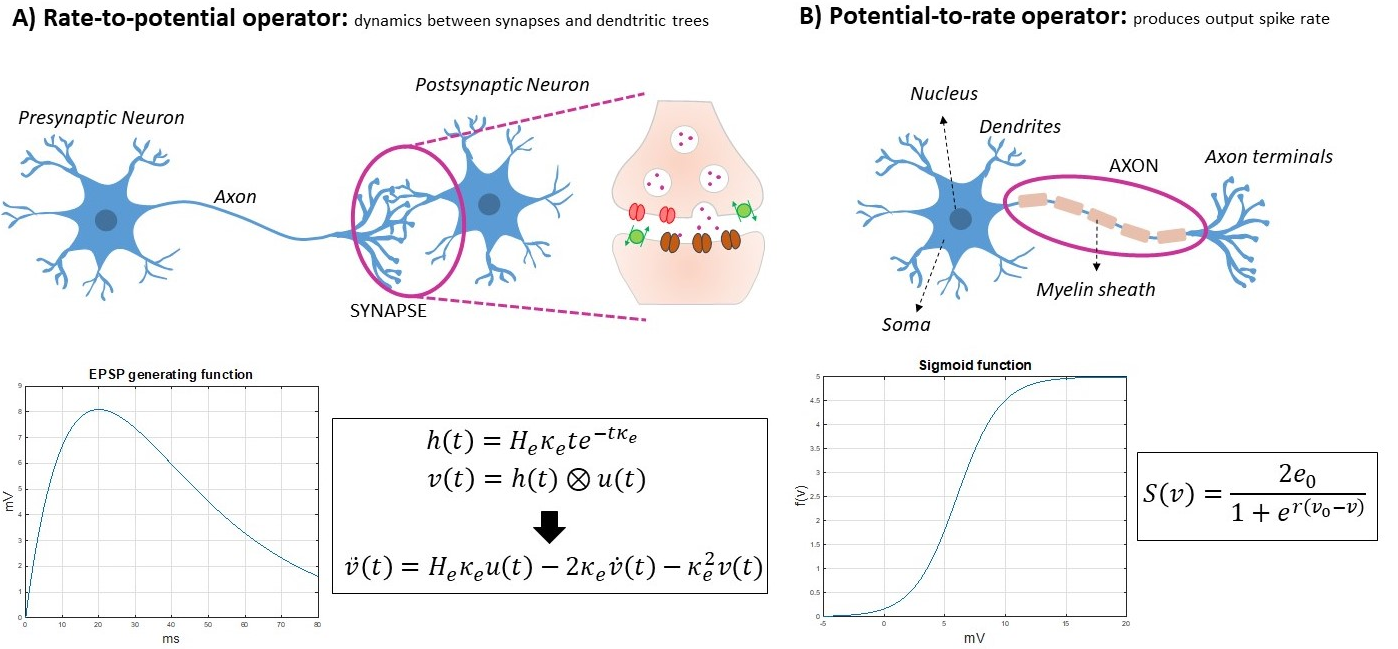
\includegraphics[width=\linewidth]{Images/Common_elem_2.png}
    \caption*{\textbf{Figure 3. \textit{Foundational components of convolution-based NMMs.}} Neural populations are composed of \textbf{A)} A rate-to-potential operator describing the postsynaptic potential generated by the firing rates of the presynaptic neurons; and \textbf{B)} a potential-to-rate operator, typically expressed as a nonlinear function, to relate the membrane potential of the neurons to their spiking activity.}
    \label{fig:Common_NMM}
\end{figure}
\vspace{-\baselineskip} 
%TC:endignore
%TC:ignore


Even though convolution-based NMM share a common framework with two core operators, three key factors sets the models apart: 1) the number of neural population modelled, 2) the degree of physiological complexity associated with each neural population, and 3) the connectivity between them. By exploring these differences, we aim to uncover how each model uniquely captures the dynamics of alpha oscillations, providing insights into the description of the underlying mechanisms. 


\section{Methods}


%\subsection{Detailed presentation of alpha rhythm NPMs} 
\subsection{Alpha rhythm models} 
%TC:endignore
With the basic conceptual and mathematical background established, the four selected NPMs representing alternative theories for the genesis of alpha activity - JR, MDF, LW, and RRW - will now be introduced in full detail. In the next few sections we present for each model i) topological and circuit diagrams with the corresponding equations, ii) alpha rhythm simulations with numerical expressions, and iii) a didactic commentary. By comparing and contrasting these models in the subsequent sections, we aim to provide insights into their activity regimes and dynamical properties. All model parameter definitions, values, and units are listed in S.9. Selected equations are included in figures to assist exposition, while the complete equations for all models can also be found in S.9, as well as in the Python code implementations in the GitHub repository accompanying this paper:\\(https://github.com/GriffithsLab/Bastiaens2024\_AlphaModels). Regarding nomenclature: originally we aimed to find a generalized mathematical form that covered all four models of interest (as in e.g. \citealp{sanz2015mathematical}), and allowed for a single and consistent set of symbols with clear correspondences across models indicated by variable and parameter names. After further exploration we determined however that this is not possible without an unhelpfully large amount of abstraction. We have therefore elected to write out the equations exactly as they appear in the original and/or primary literature sources, which are also in most cases the conventional terms used in the literature and current practice. 




%TC:ignore
\subsubsection{Jansen-Rit model}
%TC:endignore
Based on Lopes da Silva’s lumped parameter formulation \citep{lopes1974model}, the JR model was one of the first of its kind to reproduce a broad range of EEG oscillation frequencies (including alpha), as well as evoked response waveform, by describing the macroscopic electrophysiological activity within a cortical column \citep{jansen1993neurophysiologically, jansen1995electroencephalogram}. Analogously to \citet{zetterberg1978performance}, JR developed the model with three interconnected neural populations: pyramidal projection neurons ($y_0$), excitatory ($y_1$) and inhibitory ($y_2$) interneurons forming two feedback loops - a (fast) excitatory feedback loop and a slow inhibitory feedback loop (Fig. 5A; \citealp{Knösche2015}). The output  $y_1-y_2$ represents the net PSP on the pyramidal cell dendrites, which is defined as the difference between the EPSP from the excitatory population and the IPSP from the inhibitory population. This quantity corresponds to the membrane potential of pyramidal neurons, which can also be understood as the output of the columnar microcircuit that is transmitted to other adjacent and distal brain areas. Since pyramidal neurons have their apical dendrites in the superficial layers of the cortex where the postsynaptic potentials are summated, their activity is the primary contribution to the measured EEG signal \citep{jansen1995electroencephalogram, grimbert2006analysis}.  

The mathematical expression of the sigmoid for JR is defined as
\begin{equation}
     S(v)=\frac{2e_0}{1+e^{r(V_0-v)}}
 \end{equation}
 with $e_{0}$ representing the firing rate at threshold (and $2e_{0}$ the maximum firing rate), $r$ denoting the variance of firing thresholds, and $V_{0}$ the mean firing threshold. The impulse response is expressed as follows
 \begin{equation}
   h(t)=\alpha \beta te^{-\beta t}    \qquad \text{for t} > 0, 
 \end{equation}
The parameter $\alpha$ is defined as the maximum amplitude of the postsynaptic potential, and $\beta$ represents a sum of the reciprocal of the time constant of the passive membrane and all other spatially distributed delays present in the dendritic network, condensed into a single lumped term. $\alpha$, $\beta$ in Eq. 2 correspond to the terms $A$, $a$ and $B$, $b$ in Fig. 4 for the excitatory and inhibitory populations, respectively.

After transforming the impulse response in the Laplace domain, the system is fully defined by second-order differential equations (see S.1). These equations are detailed in Fig. 4B, along with the numerically integrated time series output, and the associated power spectrum in Fig. 4C.
The connectivity parameters $C_{1}$ and $C_{3}$ differ slightly from $C_{2}$ and $C_{4}$. JR assumes pyramidal cell populations synapse equally onto two other populations, but the synaptic coefficients at the dendrites of the excitatory and inhibitory populations differ. Conversely, the synaptic coefficient at the dendrites of pyramidal cells is fixed, while their synaptic connectivity changes. Thus, technically speaking, $C_{1}$ and $C_{3}$ represent synaptic coefficients, and $C_{2}$ and $C_{4}$ are connectivity constants \citep{cook2021neural}. Nevertheless, in practice all four $C$ parameters do represent connectivity strength within the columnar circuit, and can and are evaluated as such. Further details on JR equations are give in S.9.
%TC:ignore
\begin{figure}[H]
    \centering
    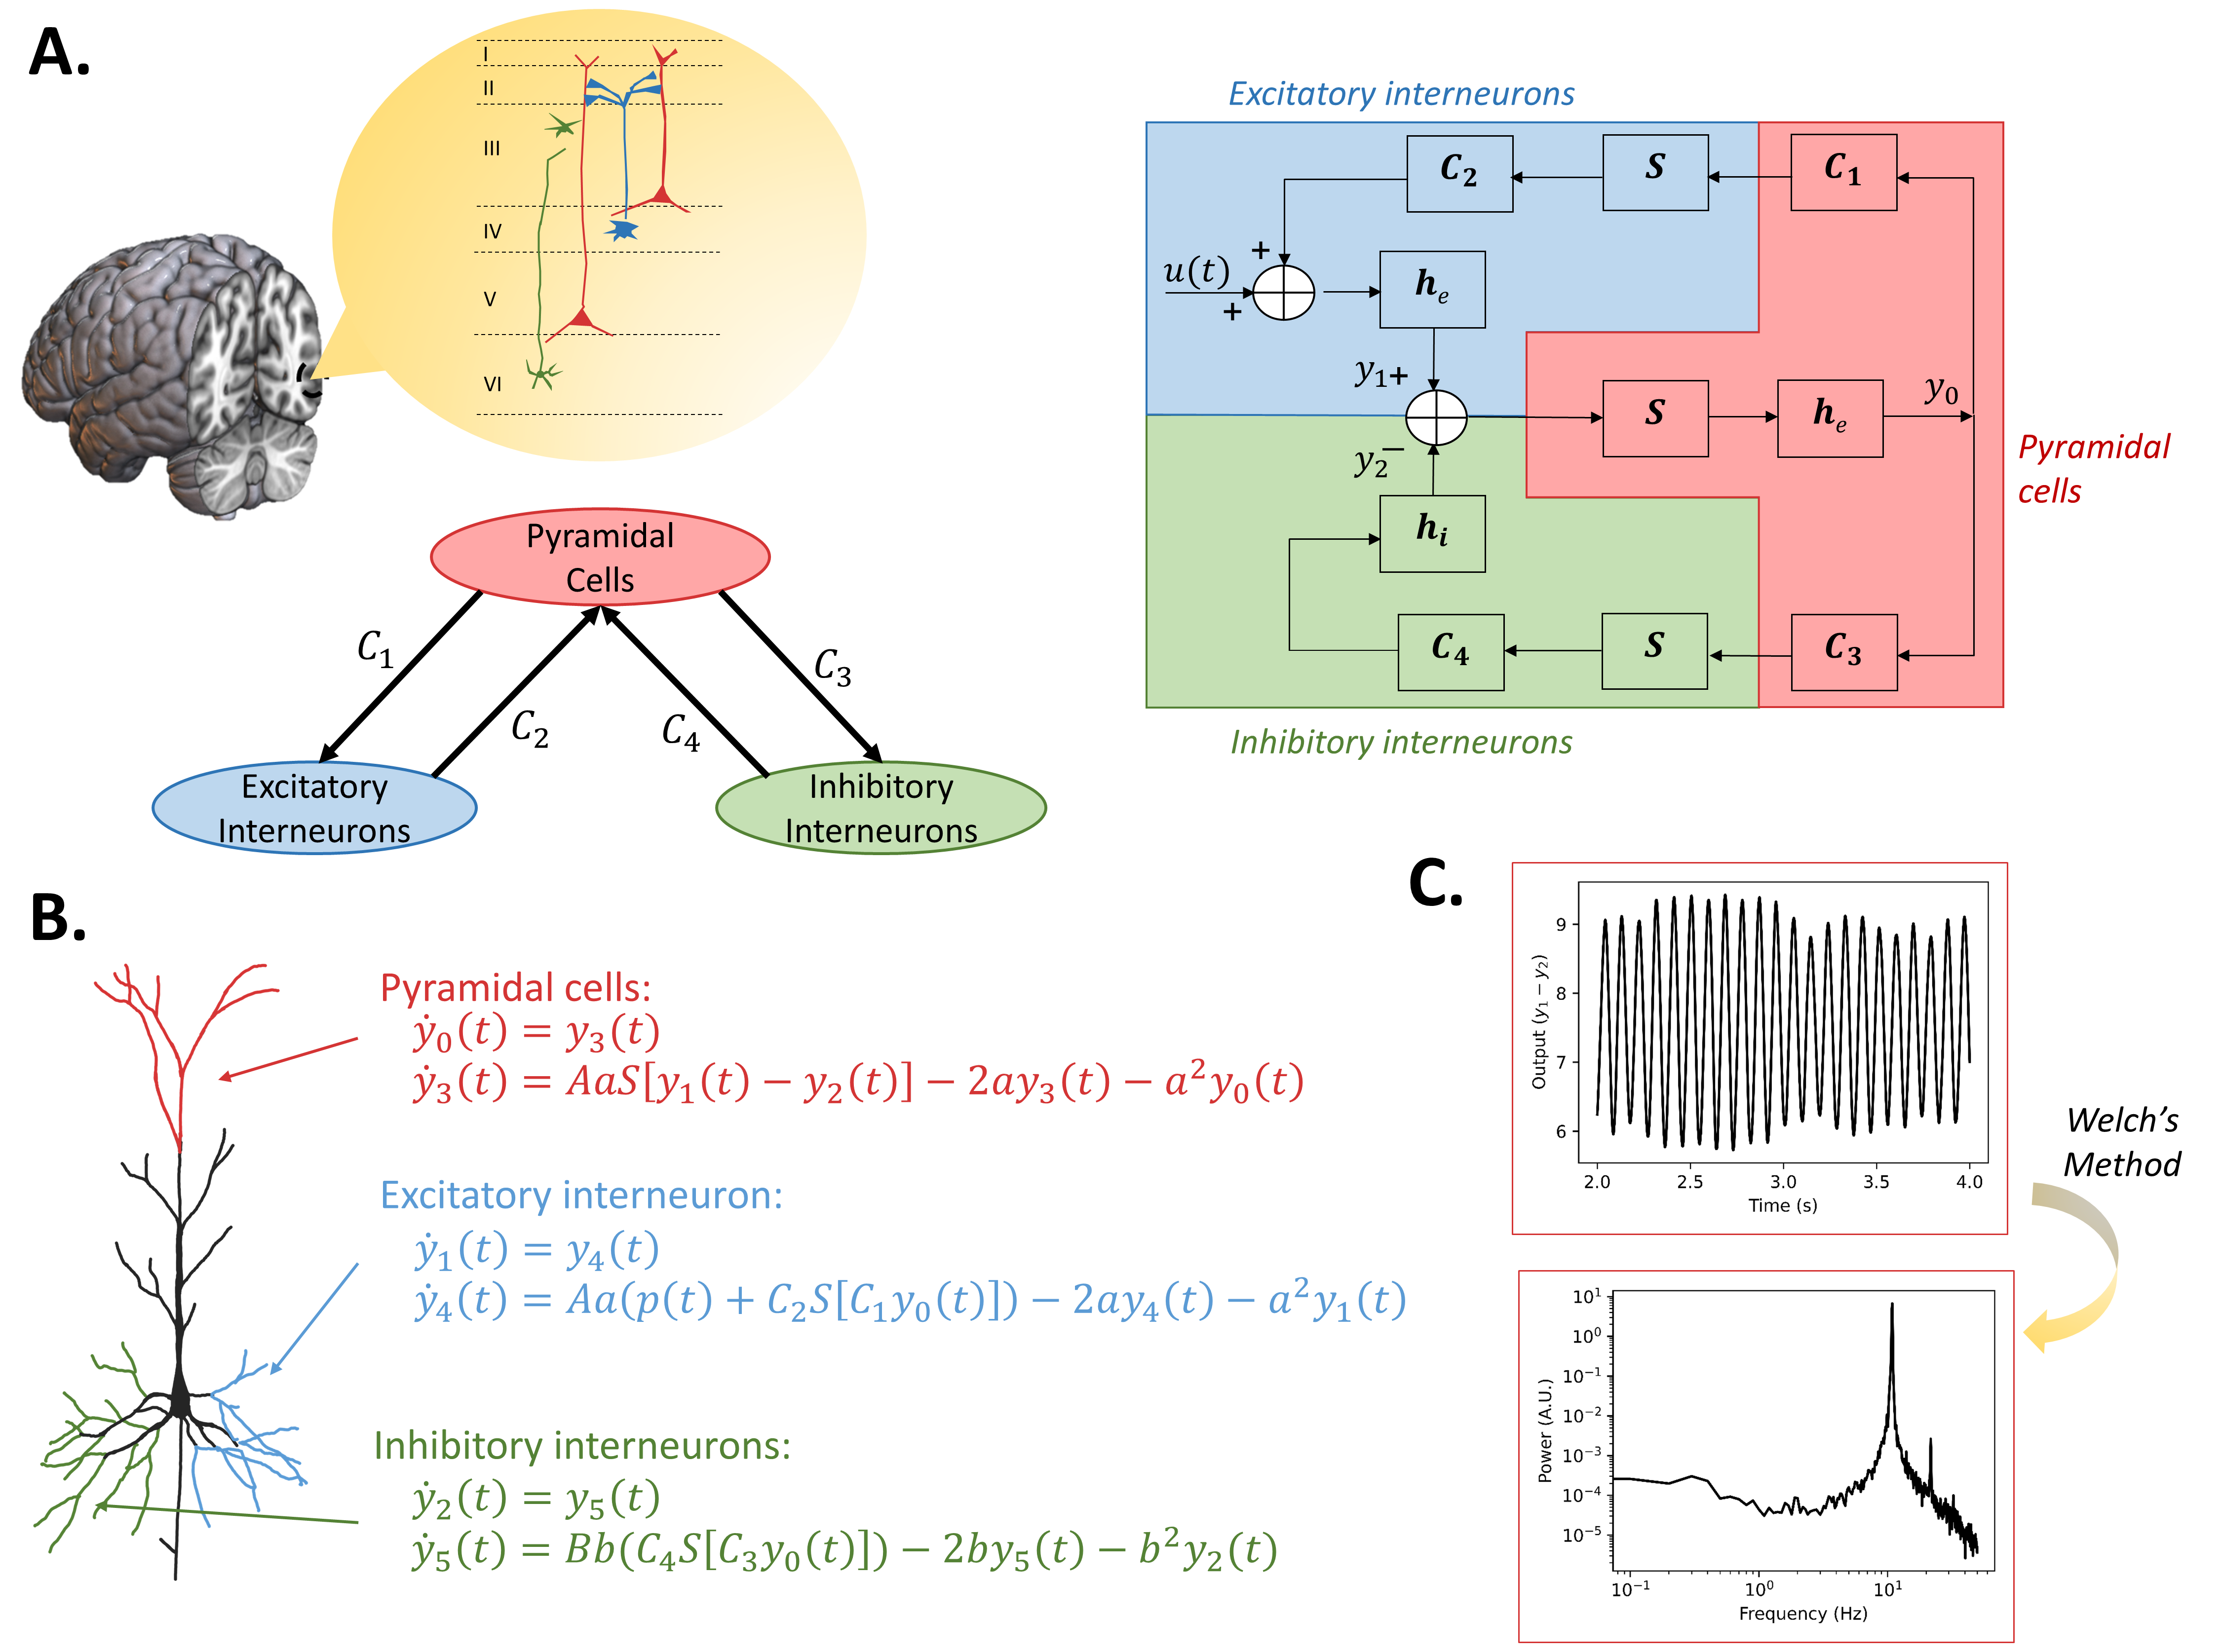
\includegraphics[scale=0.35]{Images/Jansen_rit_schematic_short.png}
    %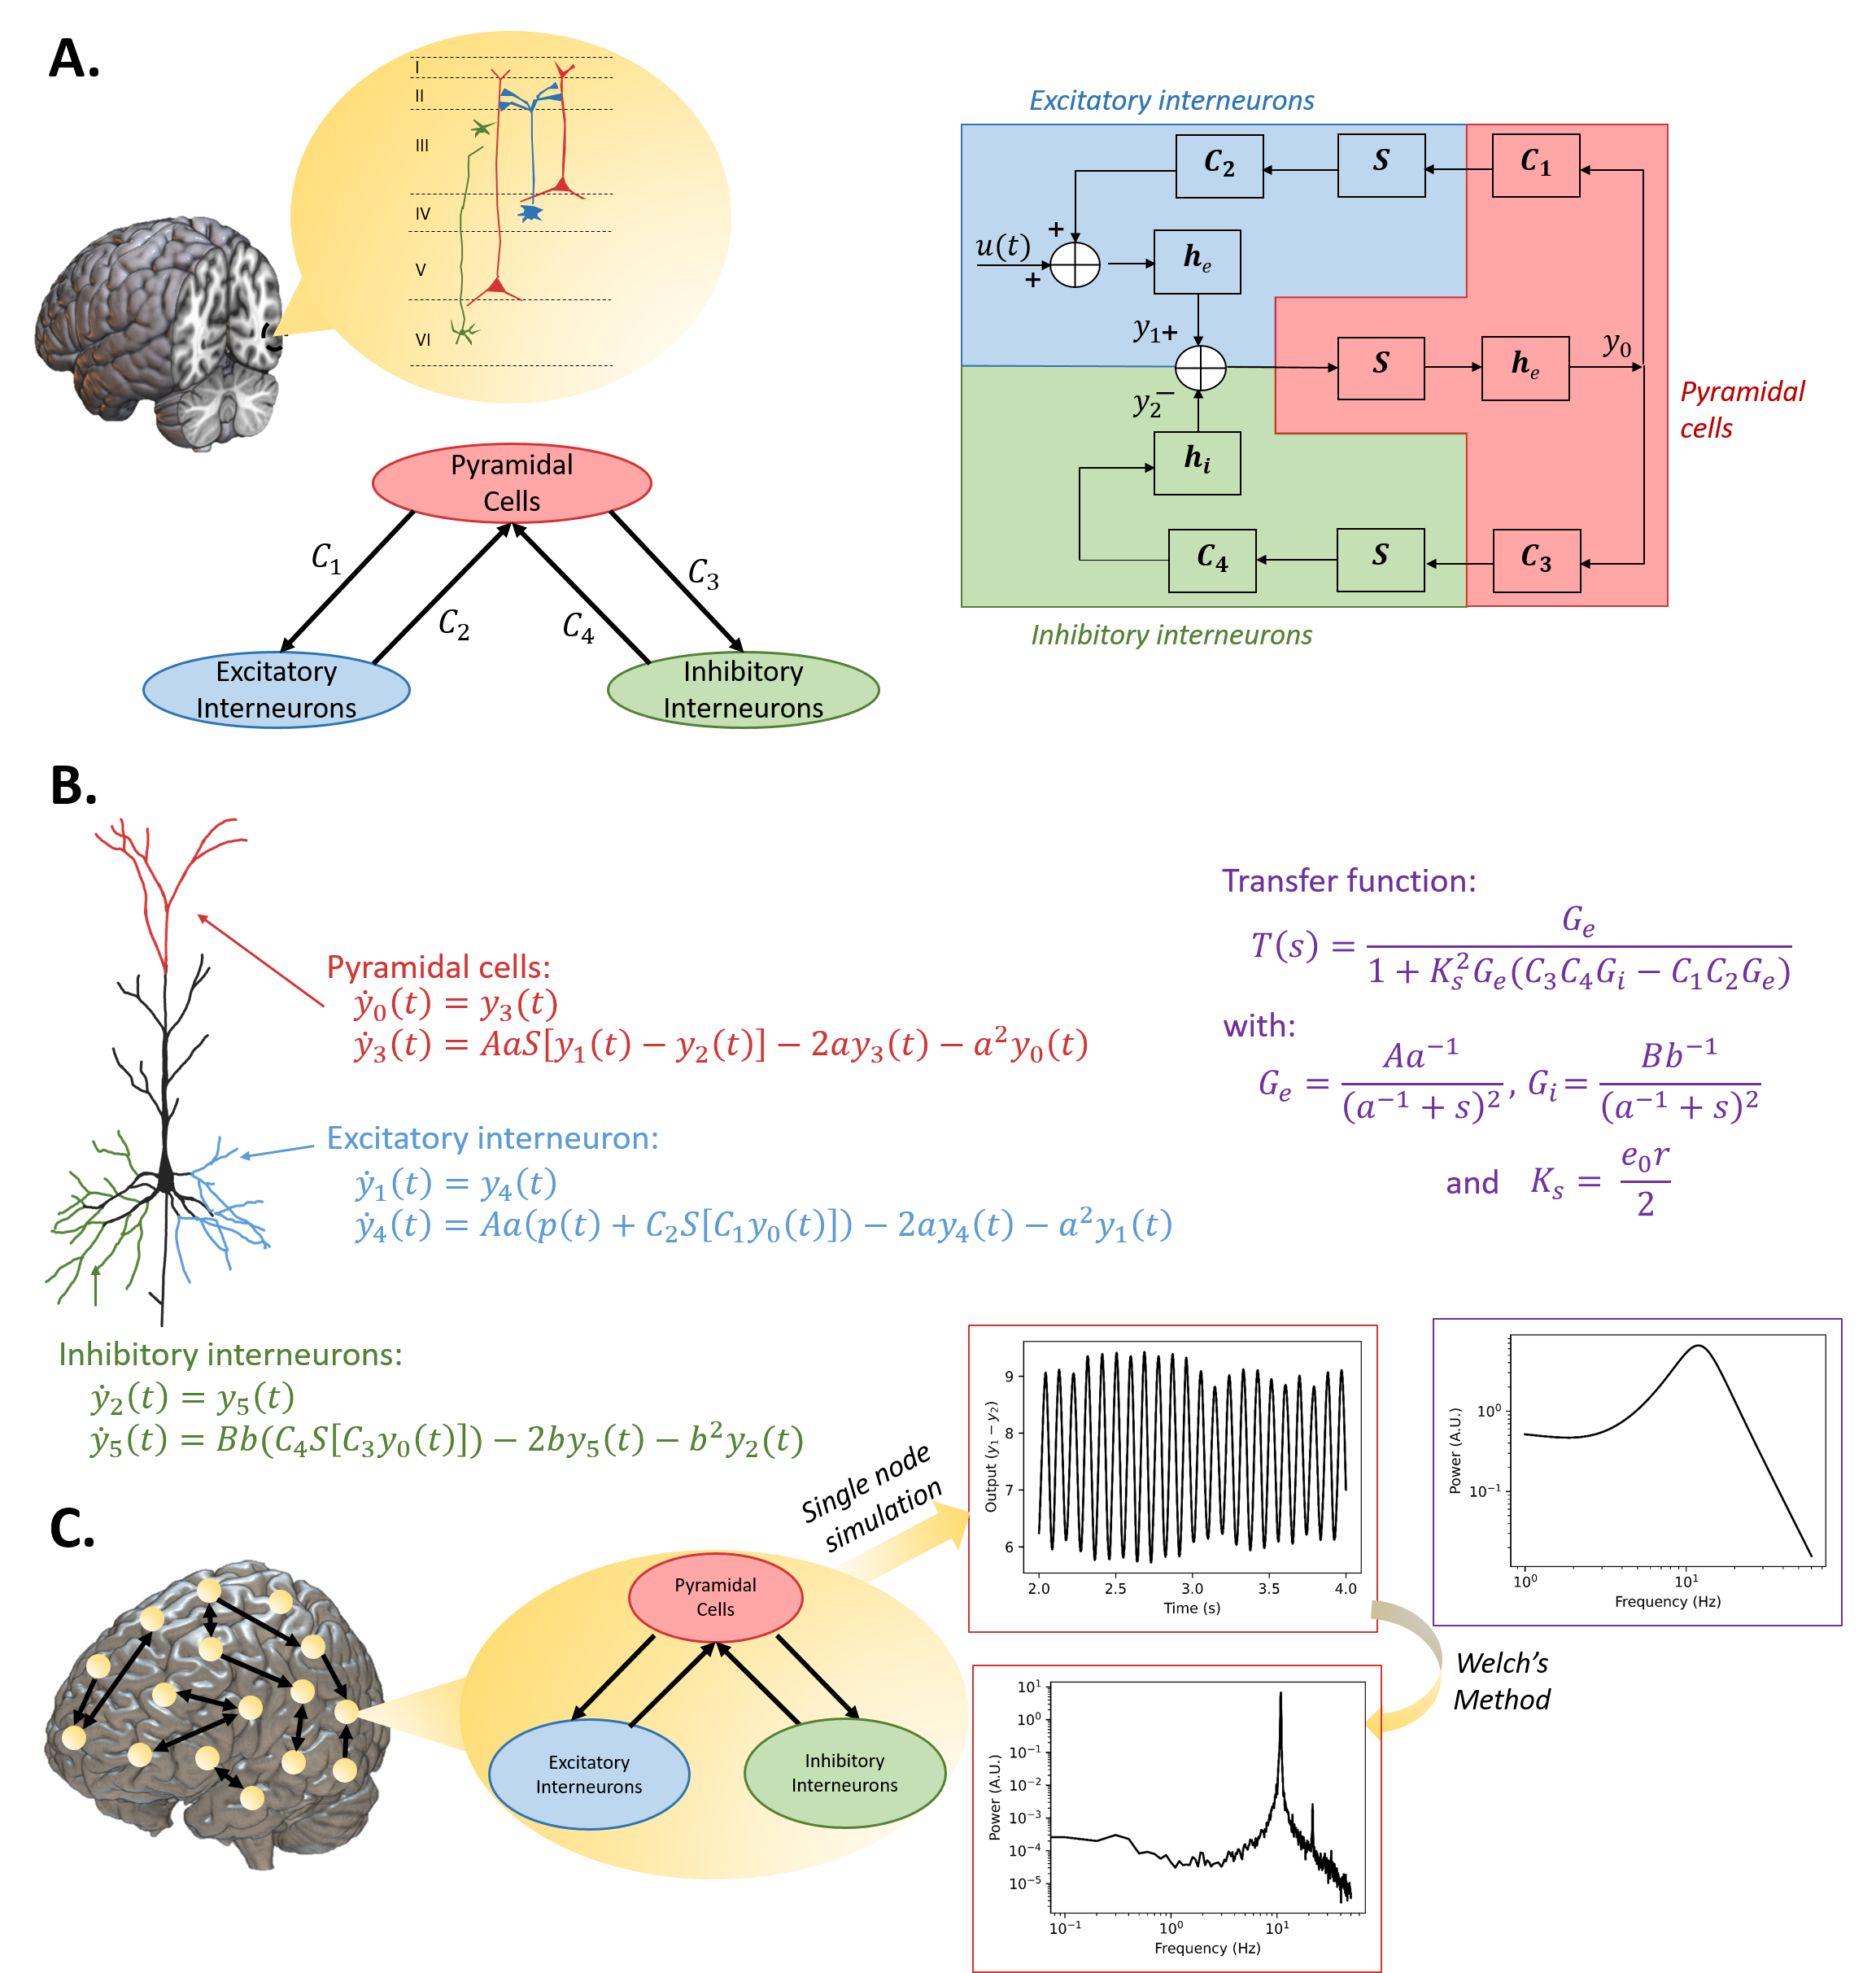
\includegraphics[scale=0.5]{Images/Jansen_rit_schematic_4.png}
    \caption*{\textbf{Figure 4.  \textit{JR model topography, schematic, numerical mathematical expression, and alpha simulation results}}. \textbf{A)} General structure of the model, along with a detailed schematic that includes the operators and representations of the connectivities; \textbf{B)} Numerical mathematical expression for each neural population \textbf{C)} Simulation outputs of the model with standard parameters (time series, power spectrum estimated from the time series)}
    \label{fig:JR_full}
\end{figure}
%TC:endignore
%TC:ignore
\subsubsection{Moran-David-Friston model}
%TC:endignore
% Chose this extension because JR is not capable of reproducing higher fr phenomena problematic to replicate neuropathology 
Many models inspired by JR emerged in the years following their introduction. One of the most influential of these was proposed by \citet{david2003neural}, later extended by \citep{moran2007neural}. The MDF model and the JR model (of which it is an indirect extension) thus share many similar features, and are interesting to compare in terms of the new elements included in \citet{david2003neural} and \citet{moran2007neural}. One such element is the addition of recurrent inhibitory connections, which were introduced by \citet{moran2007neural} in order to enable the generation of a wider range of oscillatory frequencies. Another is that the contribution from excitatory and inhibitory populations are separated in the equations, giving rise to independent EPSP and IPSP terms. The quantity used in observation models such as EEG as a measured response corresponds to the difference between these two postsynaptic potentials, resulting in supplementary sets of differential equations. A third main modifications from JR in MDF is the expression of the sigmoid, given by  
\begin{equation}
    S(v)= \frac{1}{1+e^{-\rho_1 (v-\rho_2)}}- \frac{1}{1+e^{\rho_1 \rho_2 }} .
\end{equation}
This differs from the other models surveyed in this paper (cf. Eqs 1, 4, 7) in providing a greater flexibility in its gain behavior, parameterized by  shape and position $\rho_1$ and $\rho_2$. 

The impulse response in MDF is identical to JR, and the parameters have the same definition (S.9) with some small variable name changes ($\alpha$,$\beta$ = $H_e$,$\kappa_e$ for the excitatory populations, and $\alpha$,$\beta$ = $H_i$,$\kappa_i$ for the inhibitory population).

%The paper by \citet{moran2007neural} includes a linearized version of the MDF model that is used to investigate the steady-state responses. For consistency with our analyses of the JR model, here, we have determined an alternative expression for the transfer function (Fig. 6B) using graphical stability analysis.
%TC:ignore
\begin{figure}[H]
    \centering
    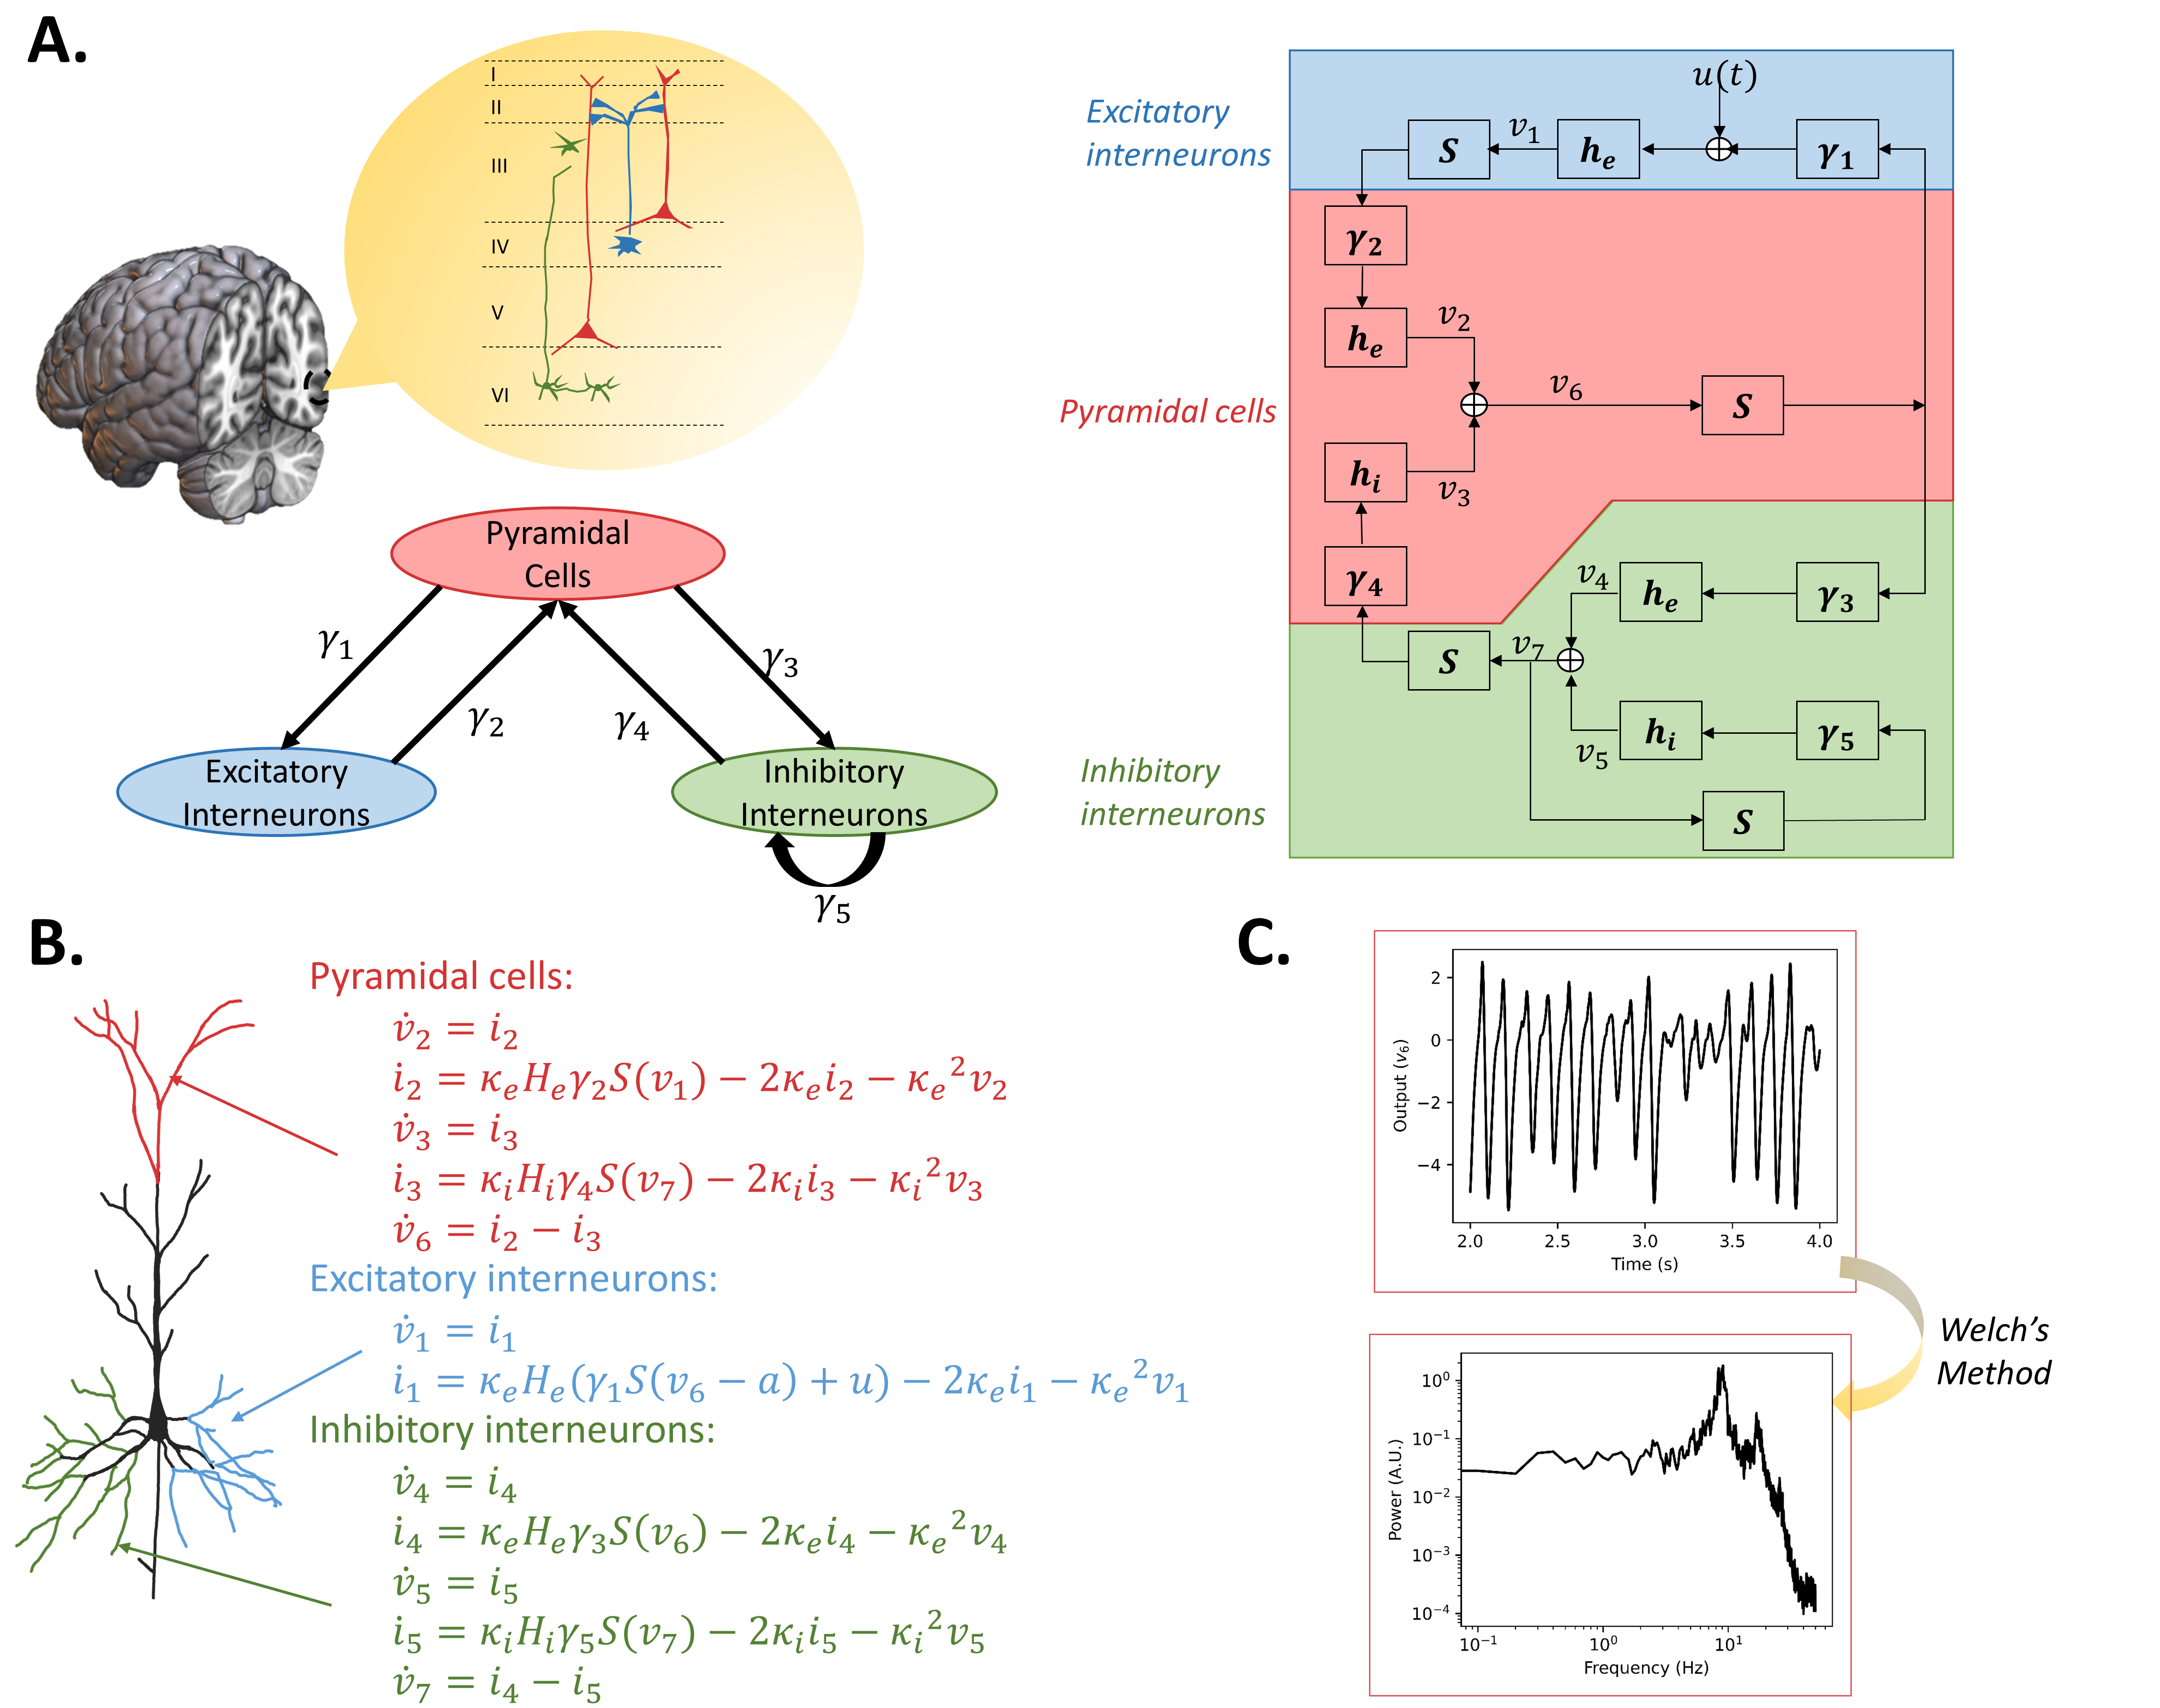
\includegraphics[scale=0.35]{Images/Moran_schematic_short.png}
    %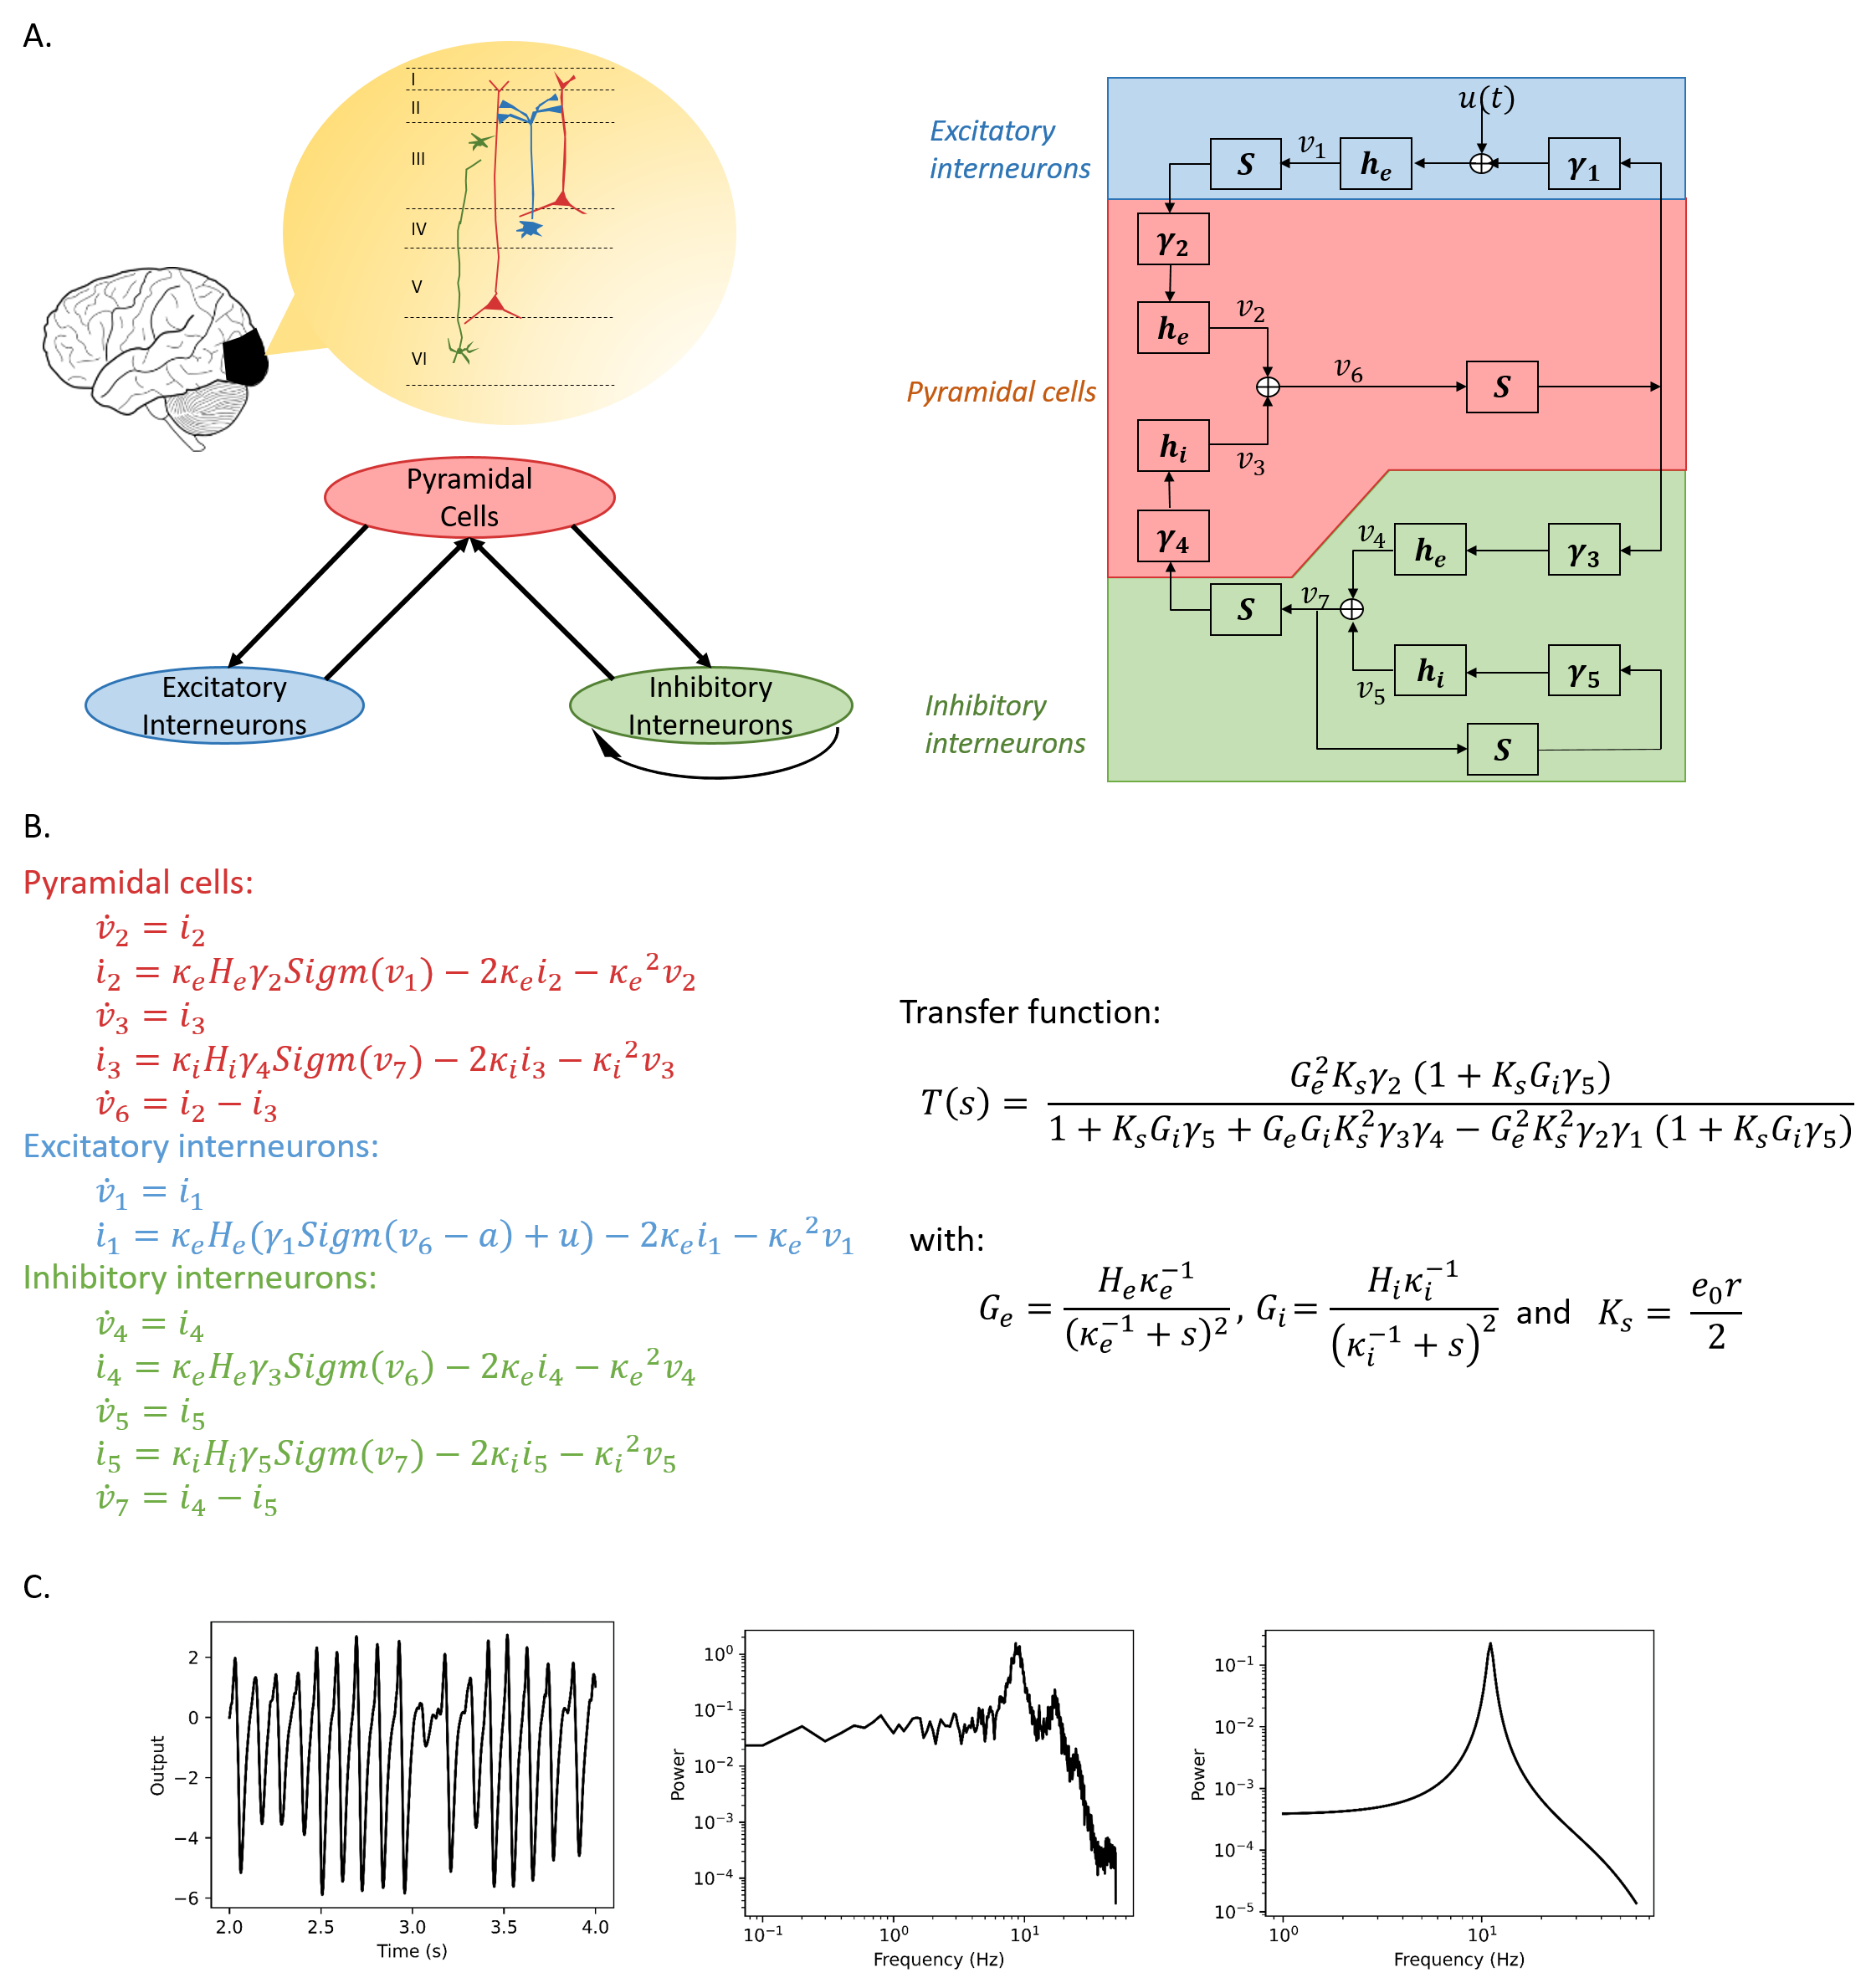
\includegraphics[scale=0.5]{Images/Moran_schematic_2.png}
    \caption*{\textbf{Figure 5.  \textit{MDF model topography, schematic, numerical mathematical expression and alpha simulation results}} \textbf{A)} Composed of three neural populations with similar wiring structure to JR with the addition of an inhibitory self-connection; \textbf{B)} Numerical mathematical expression for each neural population \textbf{C)} Simulation outputs of the model with modified parameters to generate alpha oscillations (time series, power spectrum estimated from the time series)}    
    \label{fig:Mor_topography}
\end{figure}
%TC:endignore
%\begin{figure}[H]
%    \hspace{-0.75cm}
 %   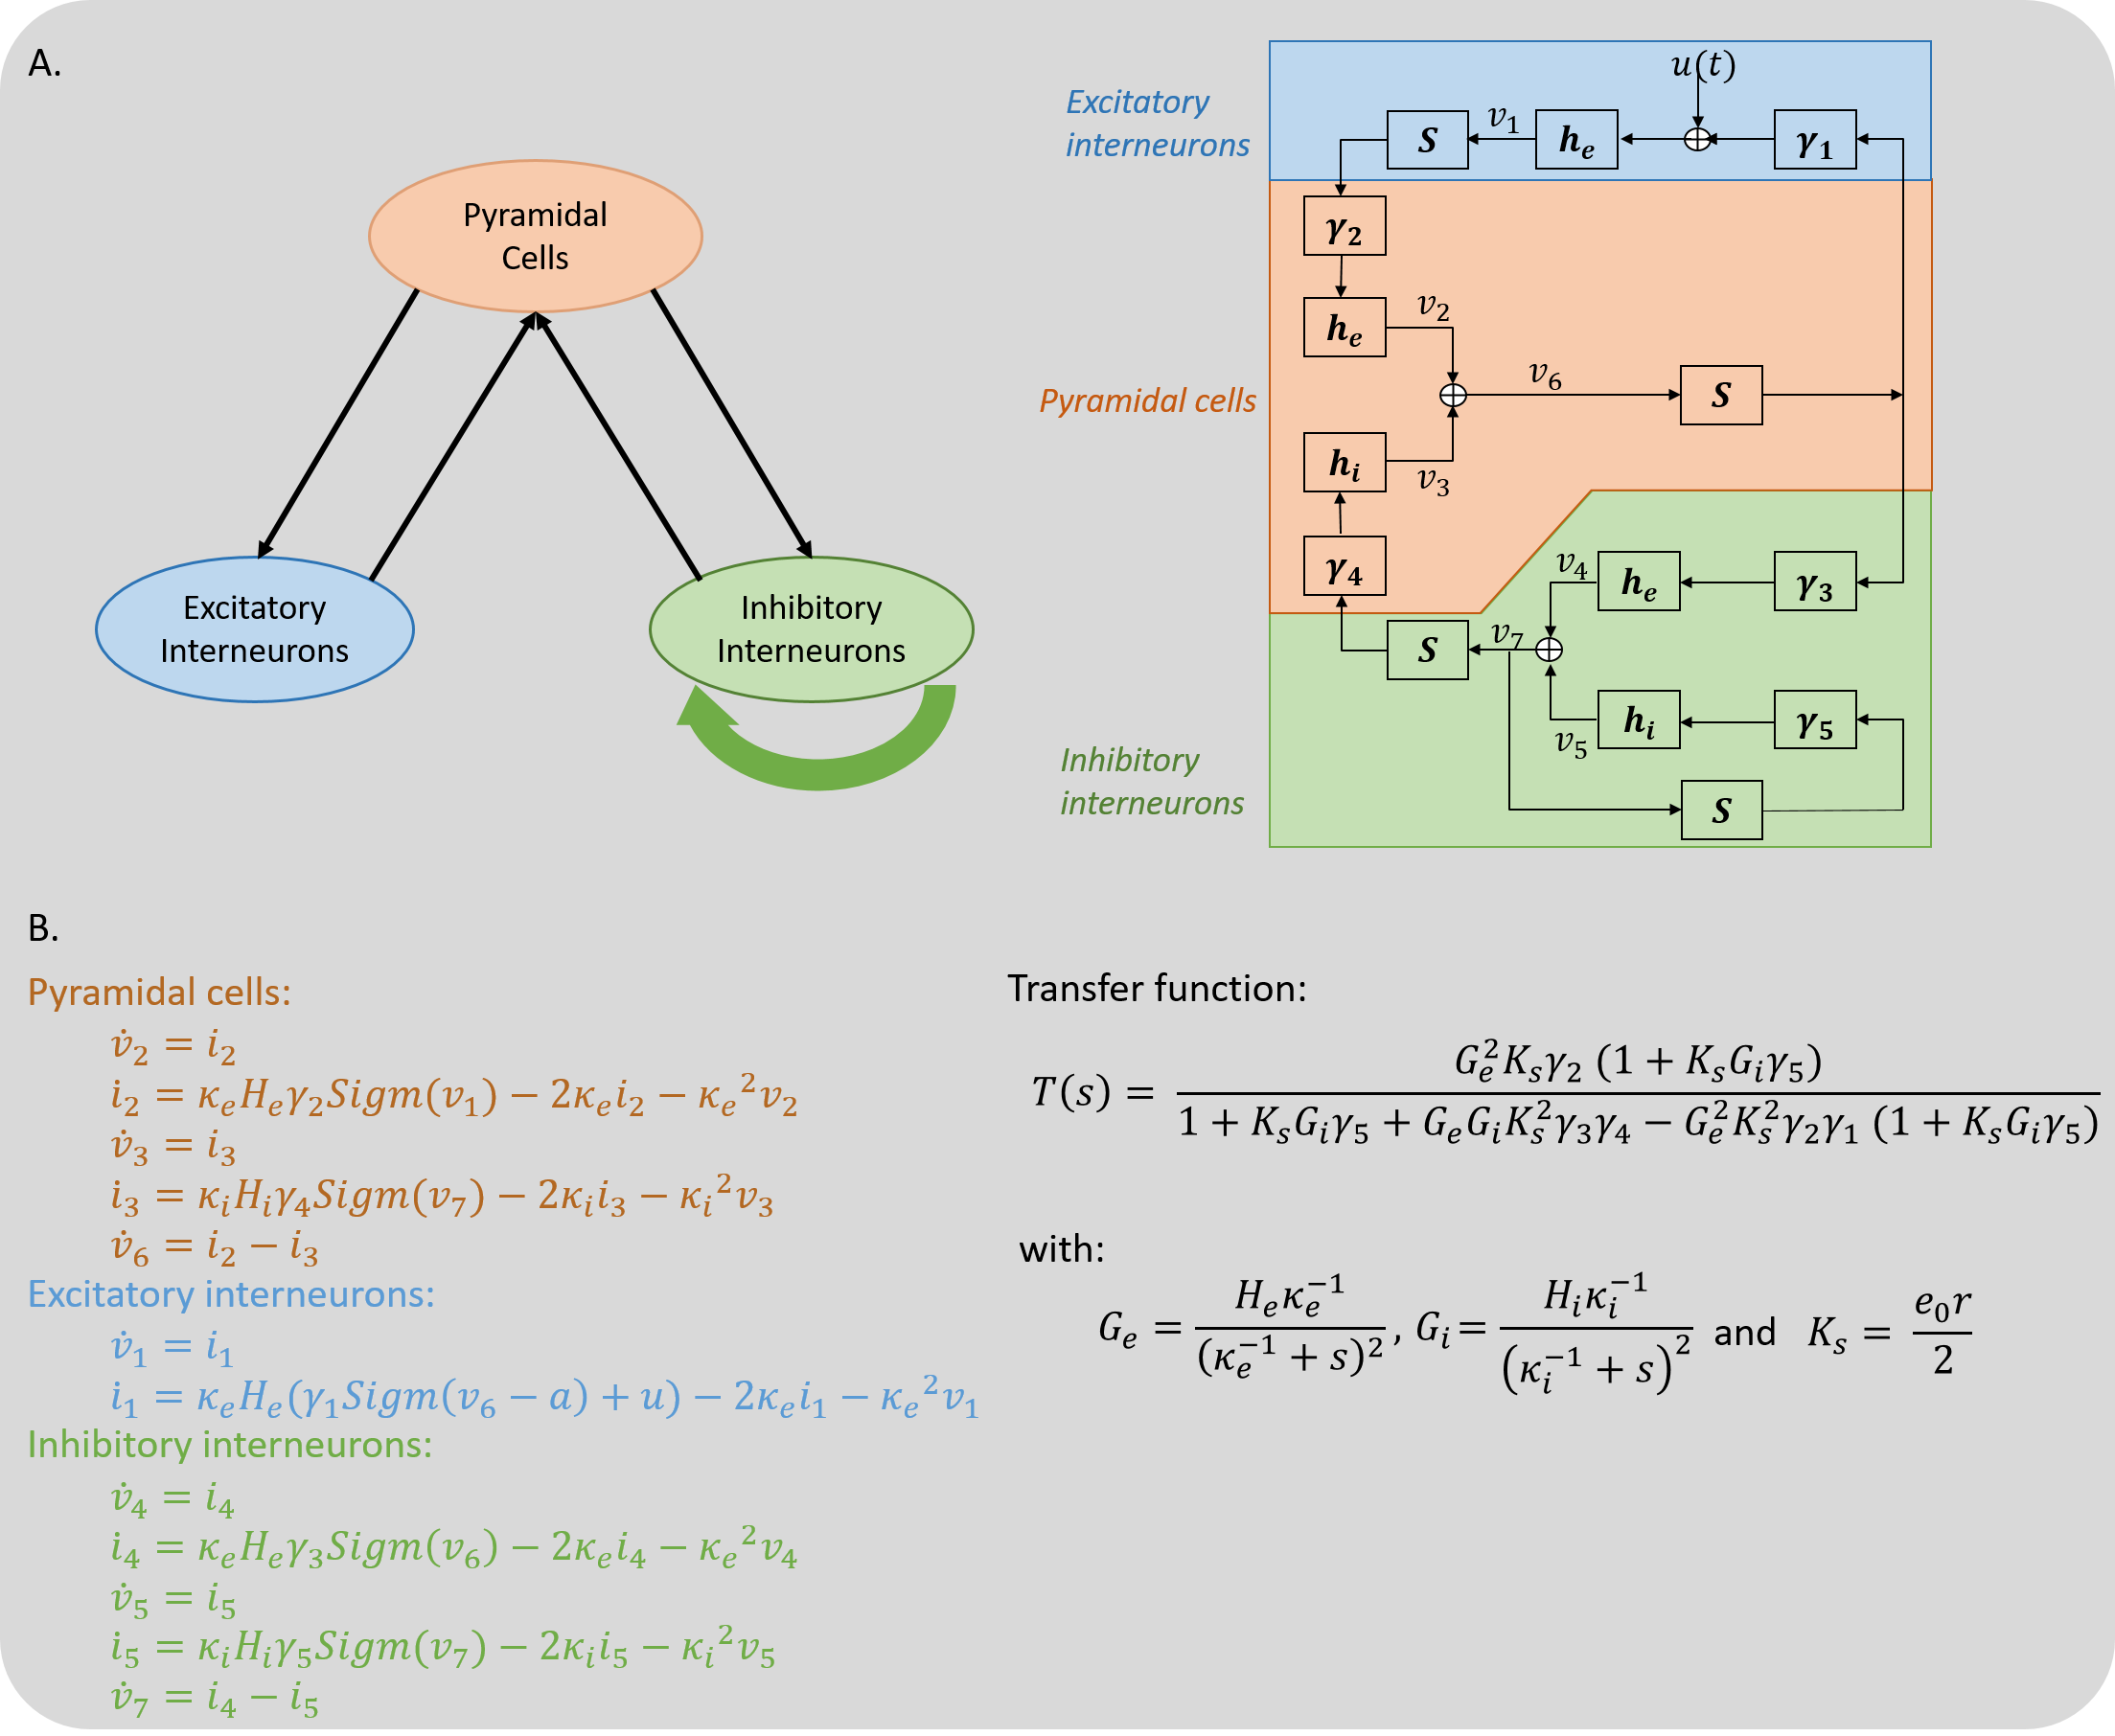
\includegraphics[scale=0.5]{Images/MR_neural_pop_summary.png}
  %  \caption*{\textbf{Figure 6.  \textit{MDF model topography and detailed schematic of interactions between three neural population.}} Composed of three neural population with similar wiring to JR with the addition of the inhibitory self-connection}    
   % \label{fig:Mor_topography}
%\end{figure}
%TC:ignore
\subsubsection{Liley-Wright model}
%TC:endignore
% From Cook: From Eq.(4.38), we can see that because conductance-based synapses are linear in both ua and Va,b, they are bilinear, which introduces another nonlinearity into the equations.

Liley, Wright, and colleagues \citep{liley2001spatially} developed a physiologically parametrizable, two population firing-rate based model of EEG/ECoG dynamics, which differs from JR and MDF in several respects. Most notably, this includes i) inclusion of high-order excitatory and inhibitory neurotransmitter kinetics, ii) presence of synaptic reversal potentials, and iii) the separation of each neural population into both a dendritic and a somatic compartment, yielding two membrane potential state variables per population instead of one. The LW model can be thought of as a convolution-based NPM with conductance-based synaptic dynamics (where a neuron is regarded as an electrical circuit and the membrane response follows the inflow and outflow of current through ionic channels). These additional features make it more physiologically realistic than e.g. JR, MDF, and WC, albeit at the expense of greater levels of complexity and nonlinearity \citep{cook2021neural}. As with the RRW model discussed below, LW was initially formulated as a macroscopic neural field model, with both spatial and temporal variation in the excitatory and inhibitory neural population equations. The version presented here is simplified, however, by neglecting spatial components (setting partial derivatives in the spatial terms of the original equations), and only considering the temporal dynamics - which nevertheless preserves the essential qualitative behavior (alpha-frequency fluctuations) that is our focus in the present paper. These expressions are based on the presentations by \citet{song2019novel} and \citet{hartoyo2019parameter}, in which LW was used to explore periodic discharges in acute hepatic encephalopathy and eyes-open/closed alpha-blocking, respectively. 

The sigmoidal firing rate function in LW is defined as

\begin{equation}
   S(t)=\frac{S_{(e,i)}^{max}}{1+e^{-\sqrt{2} (V(t)-\mu_{e,i} )/\sigma_{e,i}}}
\end{equation}

where $S_{(e,i)}^{max}$ corresponds to the maximal attainable firing rate, $\mu_{e,i}$ is the spike threshold, and $\sigma_{e,i}$ is the corresponding standard deviation. The soma membrane potential is given by 
\begin{equation}
    \tau \dot{V}(t)=V^r-V(t)+\sum \psi(V(t))I(t)
\end{equation}
where $\psi(V(t))=\frac{[V^{eq}-V(t)]}{|V^{eq}-V^r|} $, with $V_{r}$ as the mean resting membrane potential, and $V_{eq}$ the mean equilibrium potential. Similarly to MDF and JR, the impulse response in LW is expressed with an alpha function,
\begin{equation}
    h(t)=\Gamma \gamma te^{1-\gamma t}  \qquad  \text{for t} >  0
\end{equation}
with a postsynaptic potential peak amplitude $\Gamma_{e,i}$ and rate constant $\gamma_{e,i}$.

%TC:ignore
\begin{figure}[H]
    \centering
    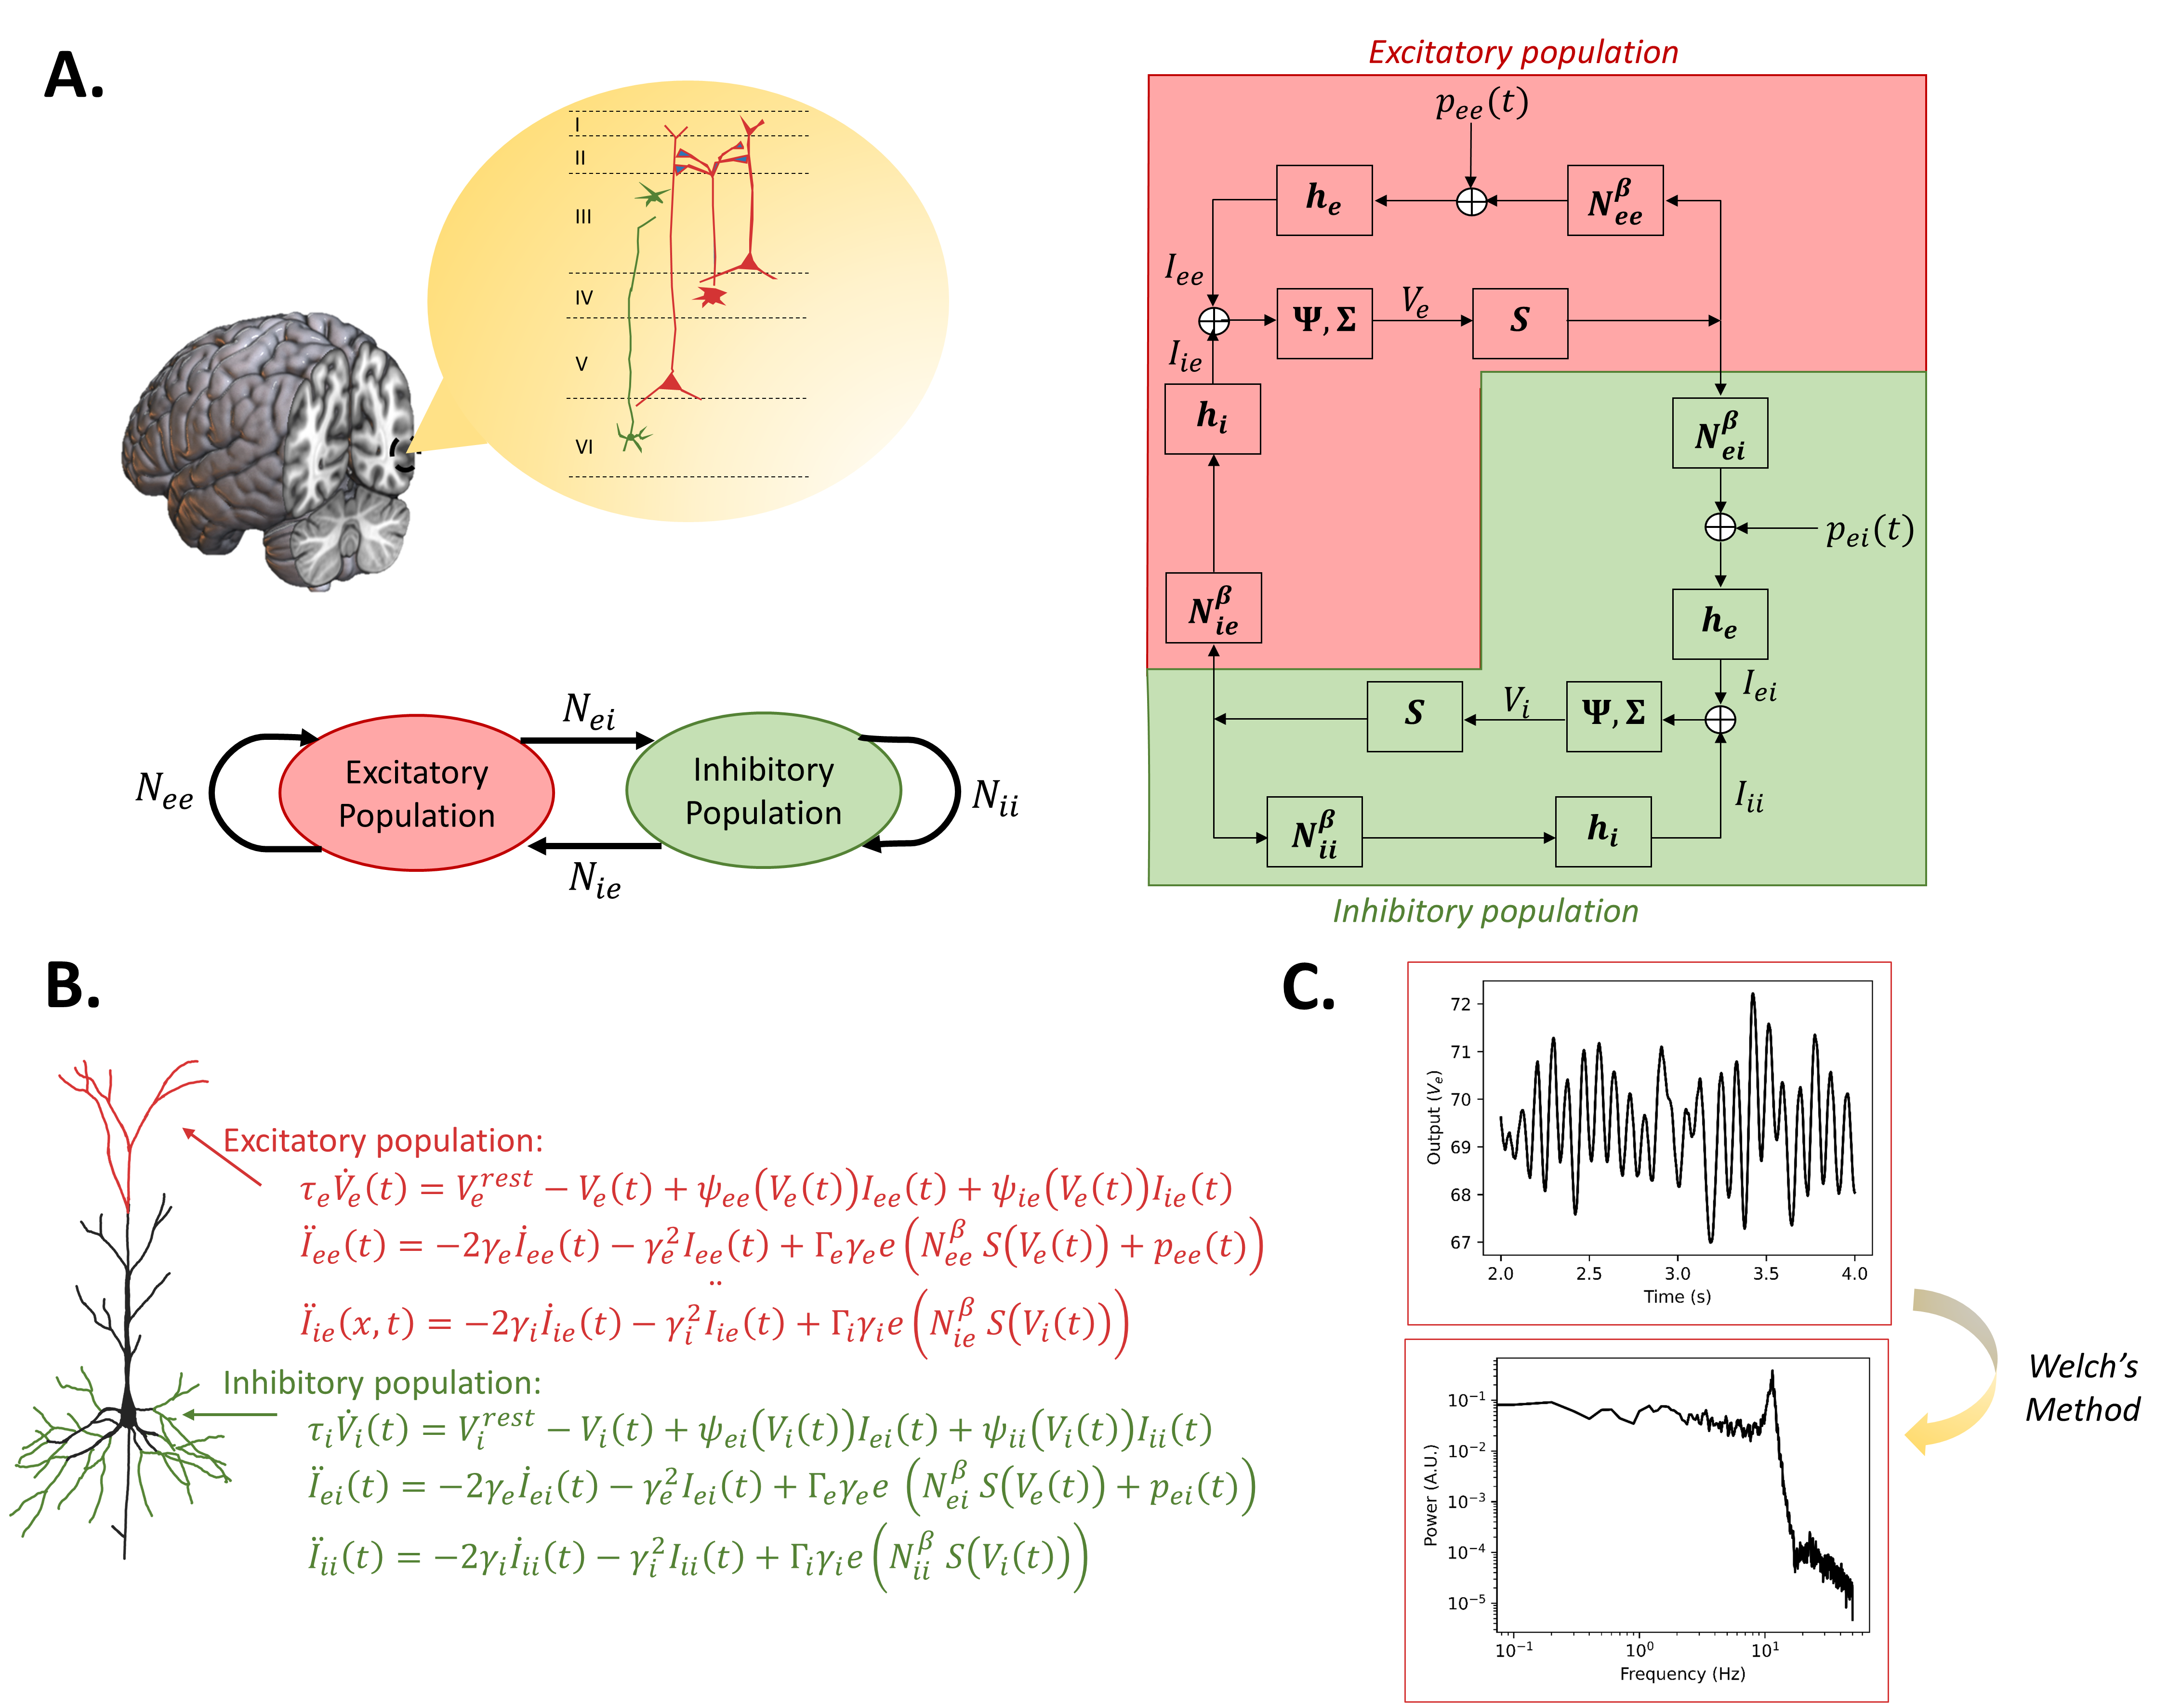
\includegraphics[scale=0.35]{Images/Liley_schematic_short.png}
    %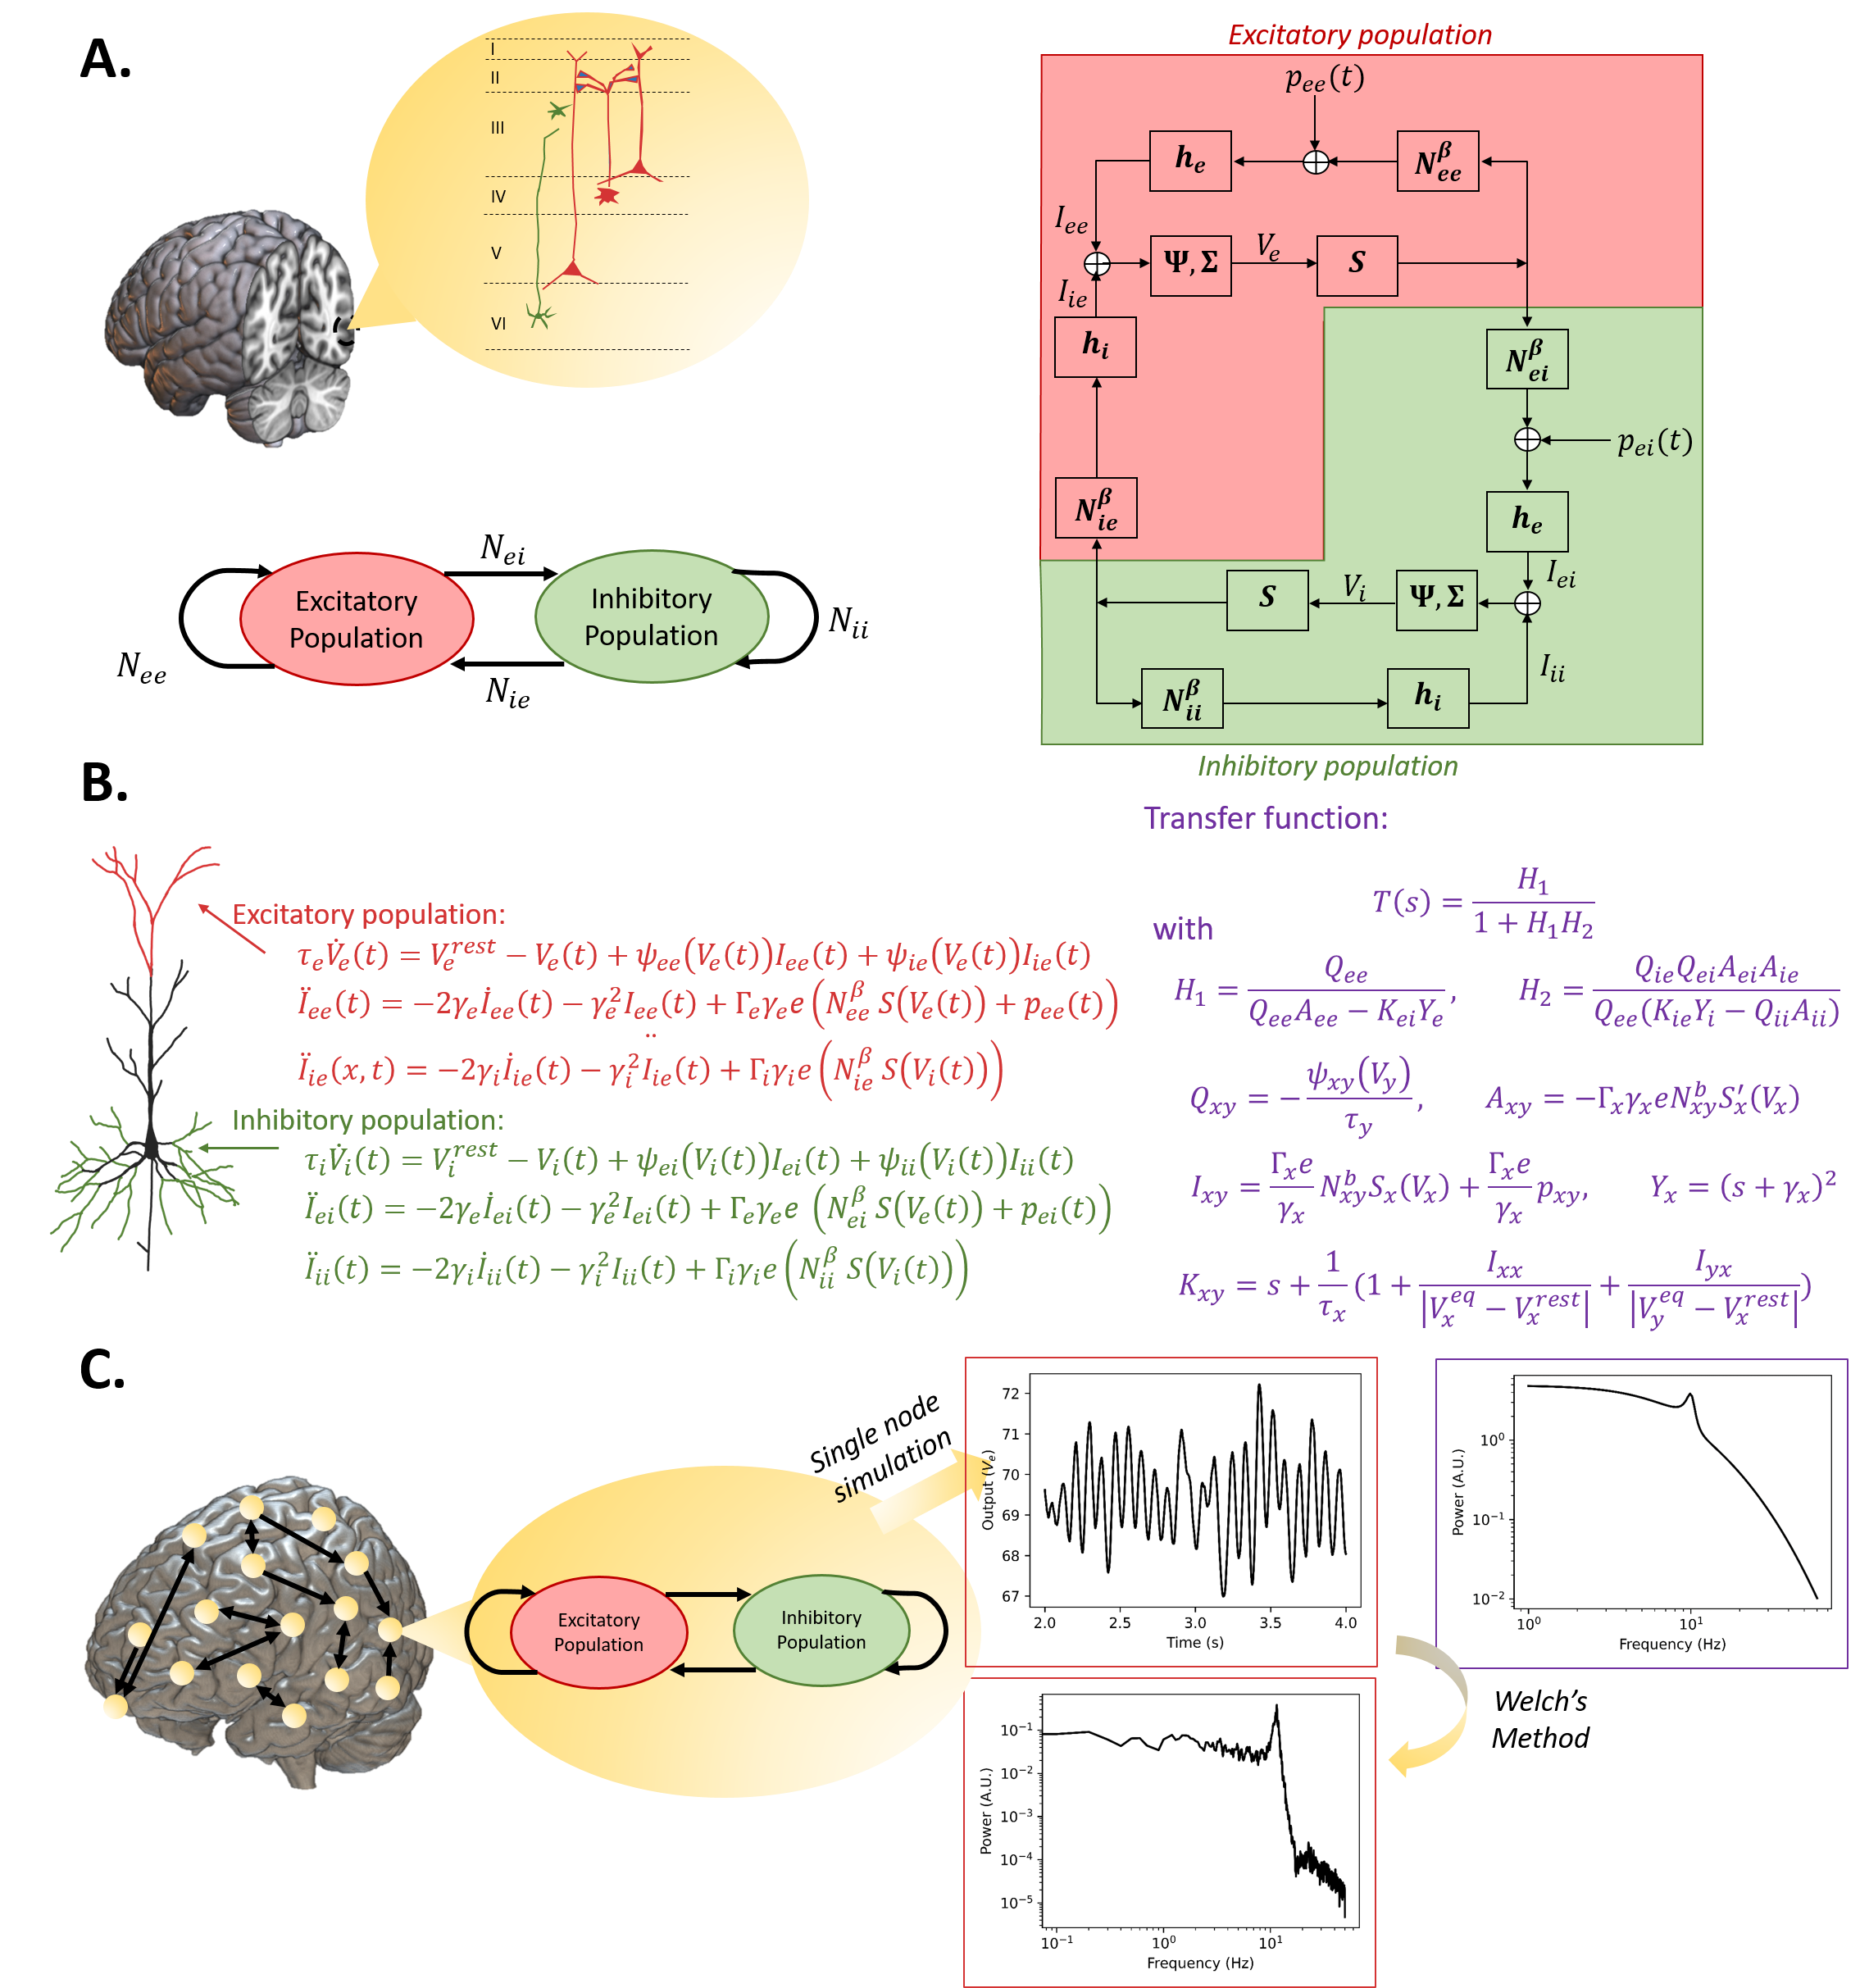
\includegraphics[scale=0.48]{Images/Liley_schematic_3.png}
    \caption*{\textbf{Figure 6. \textit{LW model  topography, schematic, numerical mathematical expression, and alpha simulation results.}} \textbf{A)} The general structure of the model is two neural populations each with a self-connection. In the detailed schematic, compared to the other models, a third block is introduced to transform PSP into soma membrane potential. \textbf{B)} Numerical mathematical expression for each neural population \textbf{C)} Simulation outputs of the model with standard parameters (time series, power spectrum estimated from the time series)
    }        
    \label{fig:Lil_topography}
\end{figure}
%TC:endignore


%TC:ignore
\subsubsection{Robinson-Rennie-Wright model}
%TC:endignore
% From cook: To investigate the spatially uniform activity, the spatially inhomogeneous term in the wave equation Eq. (4.20) is set to zero.  To make this a neural mass model, we would set the axonal range to zero rb = 0.  However, setting ∇ 2φ b(x,t) = 0 allows us to solve for the spatially uniform solutions of the neural field model.  This removes the spatial variation while still preserving the axonal range, conduction velocity and intra-cortical connectivities.

Unlike the three models discussed thus far, the RRW model does not attempt to offer a minimal circuit representation of a single cortical macrocolumn. Instead, this model includes thalamic neural populations in addition to cortical ones, and thus is primarily concerned with describing cortico-thalamic interactions. RRW permits the exploration of the second class of alpha theory outlined in Fig. 2B, which hypothesize that the corticothalamic loop is central for resting state alpha. The model consists of four neural populations \citep{robinson2002dynamics}, two cortical (excitatory and inhibitory, similar to previous schematics) and two thalamic (thalamic reticular nucleus and thalamic relay nuclei). In this case, the two cortical populations are lumped together by assuming that intracortical connections are random, making their number proportional to the number of available synapses, and implying that cortical excitatory and inhibitory voltages are equal \citep{roberts2012corticothalamic}. As noted above, like LW the original formulation of RRW is as a neural field model, making use of a damped wave equation operator for including a spatial representation. However, here we again assume spatial uniformity, removing any spatial variations, as indeed is commonly done in analyses of this model (e.g. \citealp{robinson2002dynamics, robinson2003neurophysical, van2010neurophysiological, abeysuriya2014prediction, abeysuriya2015physiologically}). Propagation effects and long axonal ranges are still preserved solely for the cortical excitatory population, this being the only population large enough with distant connections for wave propagation to have a significant effect \citep{zhao2015slow}. 
Furthermore, a corticothalamic loop delay parameter ($t_0$) is introduced to take into account the conduction delay of the signal as it passes along during corticothalamic and thalamocortical axonal projections.
The differential equations comprising RRW version we use here are given in \citet{zhao2015generalized}, who also introduced modifications to study epileptic seizures and bursting dynamics, which we omit here for clarity. The firing rate is defined as 

\begin{equation}
    Q_a=\frac{Q_a^{max}}{1+e^{-\frac{V_a-\theta_a}{\sigma_a'}}}
\end{equation}

with $Q_{max}$ representing the maximum firing rate, $\theta_{a}$ the mean firing threshold, and $\sigma_a'\pi \sqrt{3}$ the standard deviation of the threshold distribution. The damped wave equation governing long-range axonal activity propagation is expressed as

\begin{equation}
    D_a \phi_a=Q_a
\end{equation}

with $\phi_a$ corresponding to the mean density of outgoing spikes produced by population $a$, and the spatiotemporal differential operator $D_a=\frac{1}{\gamma_a^2} \frac{\partial^2}{\partial t^2}+ \frac{2}{\gamma_a} \frac{\partial}{\partial t} + 1- r_a^2 \nabla^2$ \\

In the spatially uniform case where $\nabla^2=0$, owing to the short range of cortical inhibitory axons and the relative smallness of the thalamus, $\gamma_a$ is so large that the approximation $\phi_a=Q_a$ can be made for $a=i,r,s$. This is called the \textit{local interaction approximation}, and is not assumed for $\phi_e$ as the propagation effects are significant only when considering the axons of the excitatory cortical neurons, which have significantly longer length distributions \citep{robinson2001prediction, robinson2002dynamics, sanz2017multistability}.

The impulse response in RRW includes both synaptic rise time $\beta^{-1}$ and synaptic decay time $\alpha^{-1}$ parameters, and is defined as

\begin{equation}
    \begin{aligned}
    w(u) &=\frac{\alpha \beta}{\beta - \alpha}(e^{-\alpha u} - e^{-\beta u}) \quad \text{for } \beta \neq \alpha \\
    w(u) &= \alpha ^{2}ue^{-\alpha u} \quad \text{for } \alpha = \beta
    \end{aligned}
\end{equation}

which is identical to the JR impulse response function (Equation 2) when $\alpha = \beta$, and implies that the differential equation form for the dendritic response is

\begin{equation}
    D_{\alpha \beta} =  \frac{1}{\alpha \beta}  \frac{d^2}{dt^2}+\left(\frac{1}{\alpha}+\frac{1}{\beta}\right) \frac{d}{dt}+1
\end{equation}

In the spatially uniform case, the impulse response appears as 

\begin{eqnarray}
    D_{\alpha \beta} V_e (t) &=& v_{ee} \phi_e (t)+v_{ei} \phi_i (t)+v_{es} \phi_s (t-t_0/2) \\
    D_{\alpha \beta} V_r (t) &=& v_{re} \phi_e (t-t_0 /2)+v_{rs} \phi_s (t) \\
    D_{\alpha \beta} V_s (t) &=& v_{se} \phi_e (t-t_0 /2)+v_{sr} \phi_r (t)+v_{sn} \phi_n (t)
\end{eqnarray}

%TC:ignore
\begin{figure}[H]
    \centering
    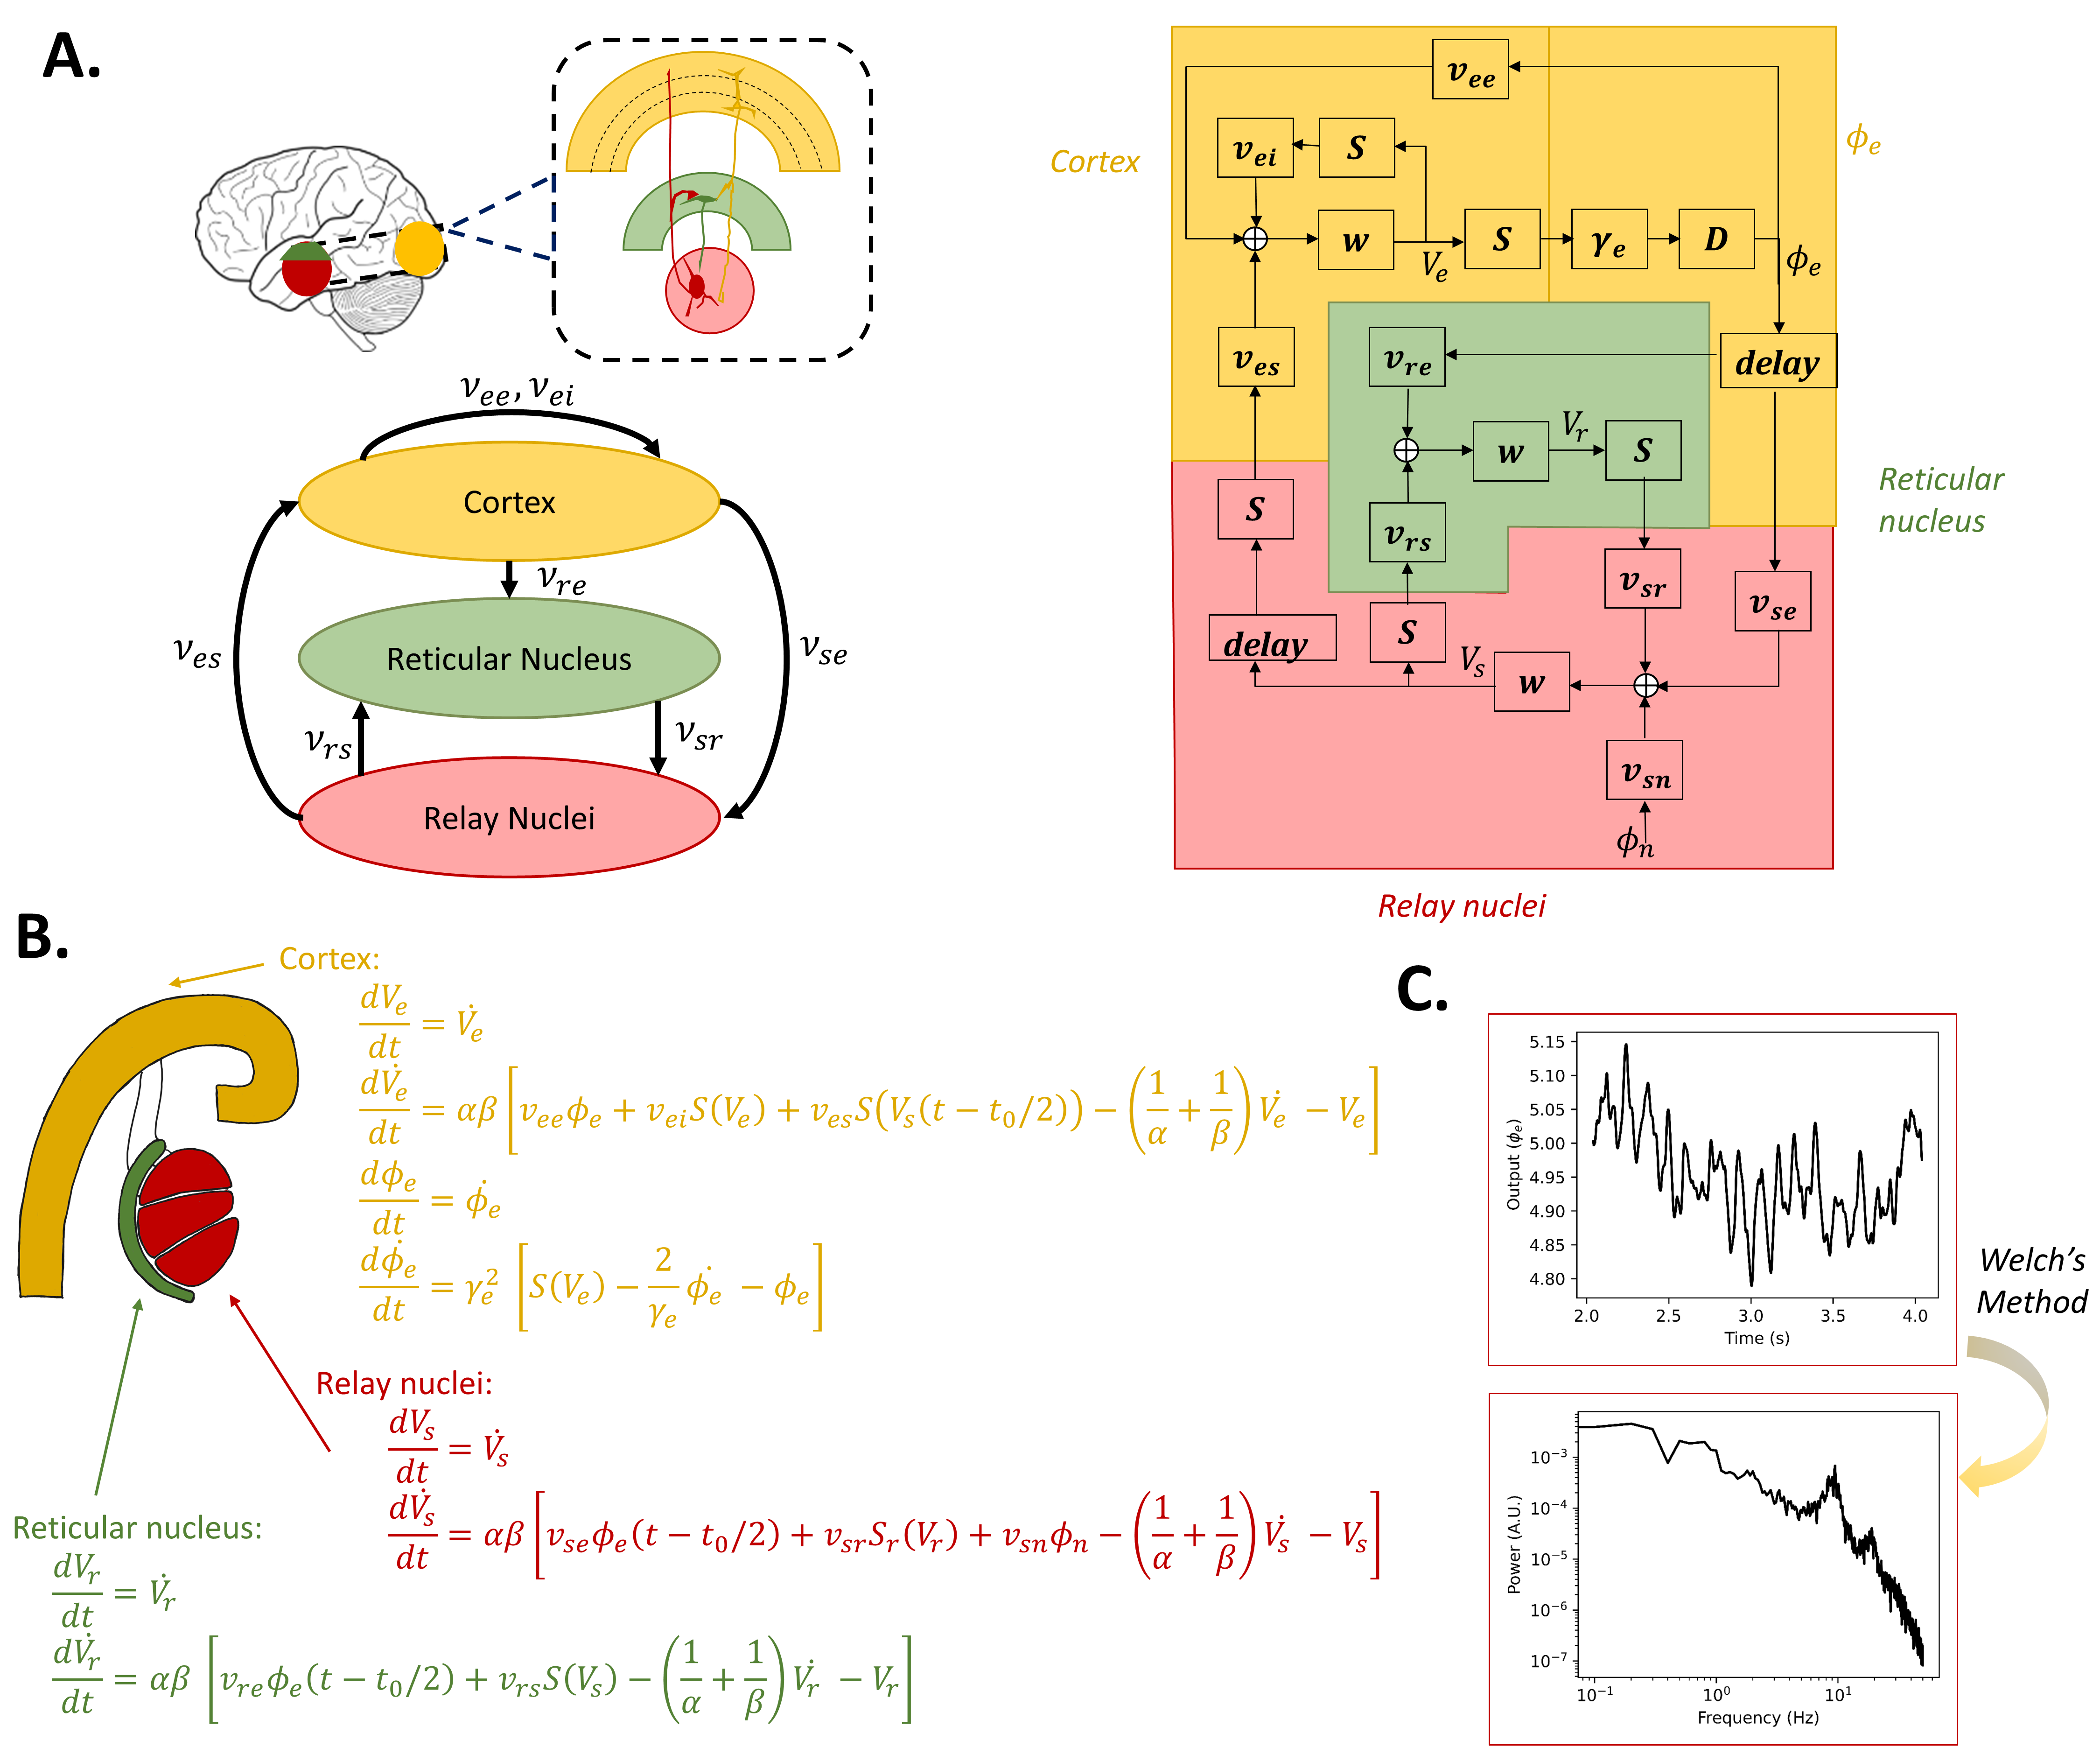
\includegraphics[scale=0.35]{Images/Robinson_schematic_short.png}
    %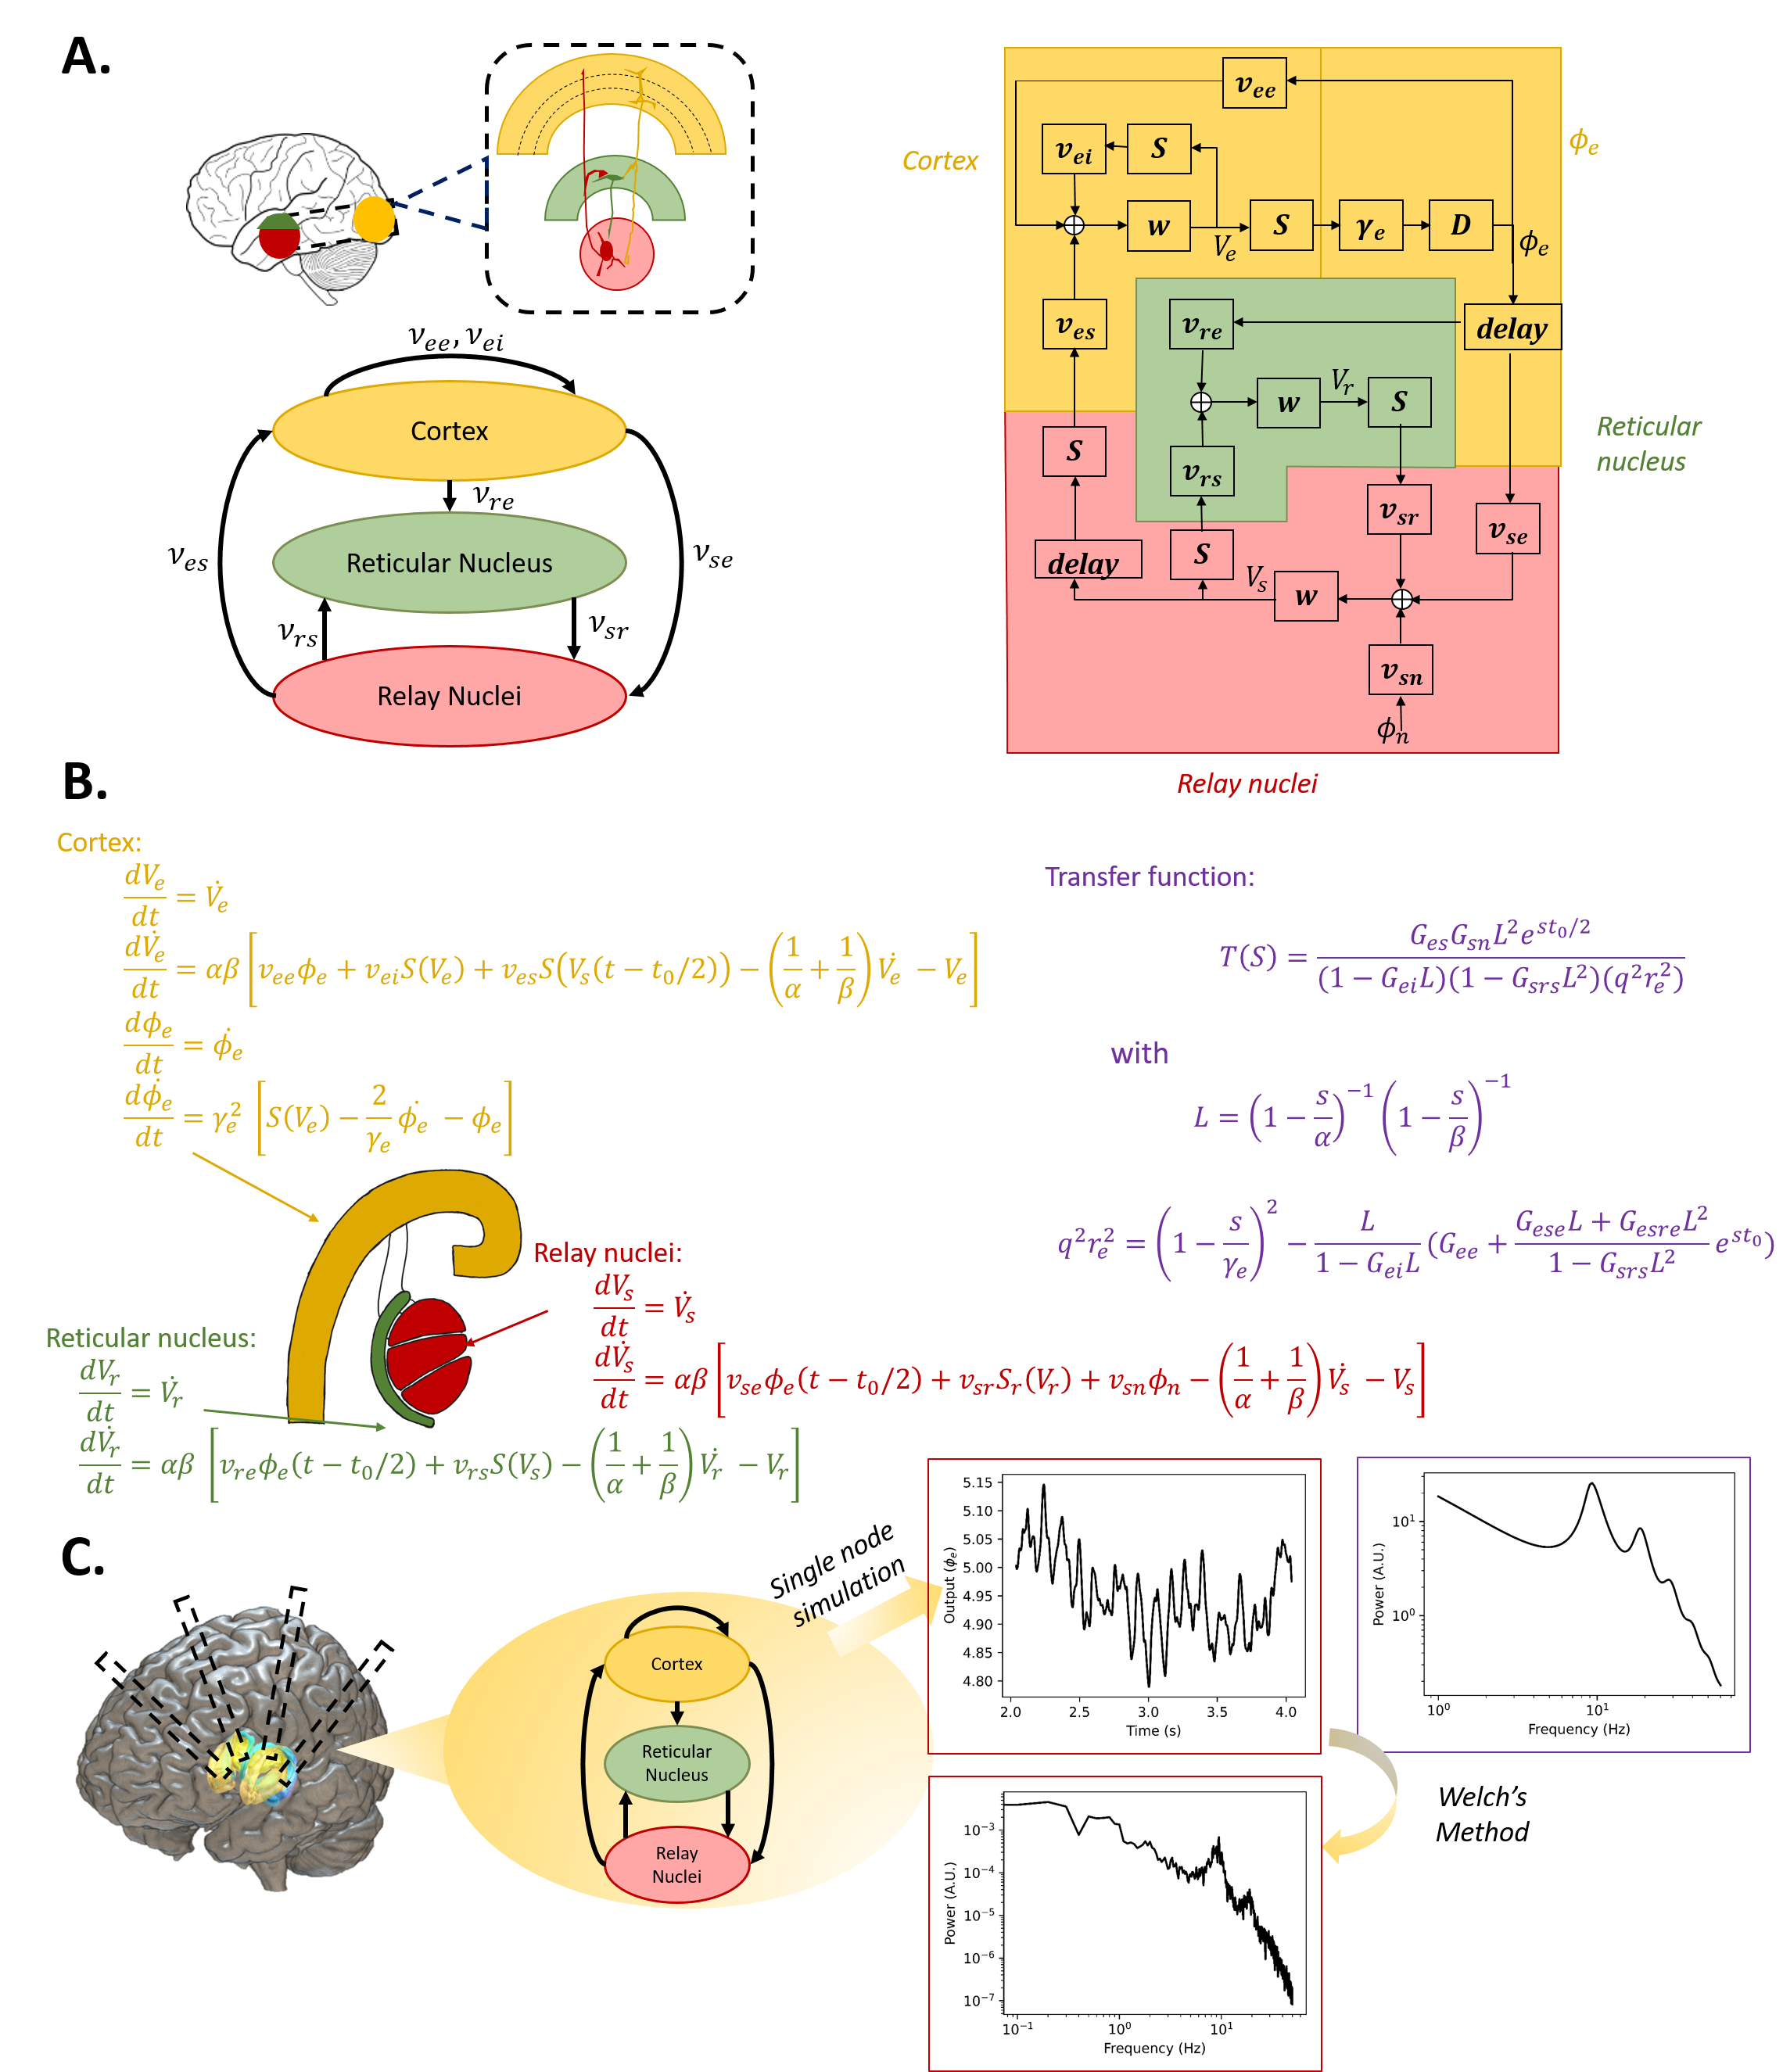
\includegraphics[scale=0.48]{Images/Robinson_schematic_4.png}
    \caption*{\textbf{Figure 7.  \textit{RRW model topography, schematic, numerical and analytical mathematical expression, and alpha simulation results.}} \textbf{A)} Three main populations are broadly described: the cortex (composed of excitatory and inhibitory neurons) and two thalamic populations (reticular nucleus and relay nuclei). Delays are included to take into account long range connections from the cortex to the thalamus; \textbf{B)} Left: Numerical mathematical expression for each neural population; Right: Transfer function of the model derived using control graph analysis; \textbf{C)} Simulation outputs of the model with standard parameters (time series, power spectrum estimated from the time series and analytical power spectrum)}            
    \label{fig:Rob_topography}
\end{figure}
%TC:endignore

% Can mention Cook again for explicit derivation of the equations 

%TC:ignore
\subsection{Simulation, power spectrum, and stability analysis methods}
%TC:endignore
For all four of the selected models, we simulated alpha activity numerically by integrating the models' differential equations given in Figs. 4-7 and S.9, and analytically, by algebraically calculating the power spectrum from the models' transfer function. Numerical simulations were run for a duration of 100 seconds, generating a time series that represents neural activity within the principal excitatory cortical population. The power spectrum of this simulated activity was then computed using Welch's method, as implemented in the scipy library \citep{2020SciPy-NMeth}. We selected parameter values commonly used in previous studies to study alpha activity, which we refer to as `standard alpha parameters': \citet{jansen1995electroencephalogram} for JR, \citet{moran2007neural} for MDF (using \citealp{david2003neural} to tune to a dominant frequency of alpha [8-12Hz] instead of beta [12-20Hz]), \citet{liley2001spatially} for LW, and \citet{zhao2015generalized} for RRW (who in turn followed from \citet{robinson2002dynamics, rowe2004estimation}). 

%Defining precise reference features of empirical alpha rhythms is challenging, due to heterogeneity both within and between individuals \citep{niedermeyer2005normal}. However, certain prominent elements of the resting state power spectral density are well-established. On average, a healthy adult human exhibits a main oscillation frequency near 10Hz, accompanied by the presence of harmonics \citep{van2010neurophysiological}. These features are considered somewhat volatile, as they significantly vary between individuals and across different sessions. 

For present purposes we focused on three reference features of empirically-measured EEG activity: i) alpha peak frequency, ii) $1/f^{\beta}$ ($\beta \approx 1 - 2$) power spectral scaling  \citep{muthukumaraswamy20181}, and iii) the phenomenon of \textit{alpha blocking} - attenuation of the alpha frequency peak during the transition from eyes-closed (EC) to eyes-open (EO) state. Each model's replication of these features was compared against reference values, taken in this case from empirical data \citet{muthukumaraswamy20181}. The exponent $\beta$ was computed with two different methods: 1) Evaluating pre- and post-peak $\beta$ separately by fitting a line with linear regression in the logarithmic scale, and 2) Using the power spectrum fit of the FOOOF library (\url{https://fooof-tools.github.io/fooof/}); \citealp{donoghue2020parameterizing}), which parametrizes neural power spectra into a mixture of the $1/f^\beta$ background and a Gaussian for each frequency peak. These FOOOF fits are also used to calculate the dominant oscillation frequencies of the power spectra, which are discussed in detail in parameter space figures of Section 3.1.2. To gain further insights into the dynamics generated by JR and LW, we determined the stability of the fixed points of the system as a function of E-I connection strengths, the derivations of which are given in S.3). Python (3.8) code for all signal processing and modelling analyses is available at \url{https://github.com/GriffithsLab/Bastiaens2024\_AlphaModels}. 
%The aim of our numerical explorations of these models in the following was to determine 1) to what extent do they 
%accurately capture empirical EEG alpha rhythms, 2) how do rate constant and connectivity parameters influence the alpha activity regime and the broader system dynamics, and 3) what are the limitations of these models, and what do the differences between them imply for theories of EEG alpha rhythmogenesis.
%TC:ignore
\section{Results}
%TC:endignore
Having presented and contrasted the four candidate alpha models (JR, MDF, LW, RRW) in terms of their motivation and formulation, we now turn to an assessment of their simulated activity dynamics. First, we present numerical and analytic spectra, discussing general characteristics and comparing them quantitatively against empirical EEG features. Second, an exploration of the boundaries of the alpha regime is conducted through parameter searches, with a specific focus on discerning the impact of rate constant and connectivity on the dominant oscillation frequency. Last, a comprehensive comparison of the models is provided, encompassing various facets including their topology, mathematical equations, and the biological significance attributed to the parameters.
%TC:ignore
\subsection{Analysis of neural model dynamics}

\subsubsection{Characteristics of model-generated alpha activity}
%TC:endignore
%SOURCES FOR 1/f empirical EEG from Moran paper: m (Barlow, 1993; Jirsa and Haken, 1996; Robinson, 2005)
%The ability and accuracy of the model to replicate an empirical alpha rhythm is explored by running the numerical simulation using standard parameter values identified from literature and comparing the resulting power spectra against characteristic empirical resting-state EEG features. For consistency, all simulations are run in Python for 100 seconds outputting a time series representing the voltage neural activity of the principal excitatory cortical population. The power spectrum is then estimated using scipy Welch's method. For the JR model, nominal parameter values are from Jansen et al. 1995; for MDF model, Moran et al. 2007 and David and Friston 2003 to generate a dominant frequency of alpha instead of beta; for LW, Liley et al. 2002; for RRW, Robinson et al. 2002, 2004 and Zhao et al. 2015. 


%For the numerical expression, differential equations are solved with the Euler method for Jansen-Rit and Moran (which are using uniformly white noise) and the Euler-Maruyama method for Liley and Robinson (which are stochastic models with normal white noise).%check 
%and the power spectrum is estimated from the time series using Welch's method. For the analytical expression, the transfer function is representative of the power spectral density. The input and parameter used are summarized in table (put ref) and further discussed in the next section. Figure 12 shows the resulting power spectrum in each case. In each case, a peak in the alpha frequency range is observed, but variations in shape, amplitude and 1/f noise are observed. With those simulations, it is possible to compare against experiment occipital EEG recordings. However,  On average, . the amplitude is less than 50$\mu$ volt and shape of 1/f.



%A main frequency of oscillation is observed in the alpha range for each of the models with values of 10.8, 11.6 and 9.5 for JR, LW and RRW respectively (Figure 9A). The closest to 10Hz is JR, with LW a slightly higher value and RRW lower value. However, all these values fall well within the alpha oscillatory range (8-12Hz), and thus can be considered to adequately simulate the alpha frequency peak since significant heterogeneity exist across subjects not only in terms of the central frequency but also in terms of magnitude \citep{haegens2014inter}. Furthermore, slight modification in the parameters can shift the peak frequency towards 10Hz. Harmonics are present in each model but they are the least accentuated in the LW model. In the linearized version, no harmonics are seen expect for RRW. 

\paragraph{\textit{Frequency peak and harmonics}}~\\
Each of the models displays a dominant oscillatory frequency within the alpha range for the originally-reported default parameters, with values of 10.8Hz, 8.8Hz, 11.6Hz, and 9.5Hz observed for JR, MDF, LW, and RRW, respectively (Fig. 8A). With these parameter settings, JR closely approximates the 10Hz frequency, while LW demonstrates a slightly higher value, and RRW a lower value. Importantly, all of these frequencies fall well within the alpha oscillatory range of 8-12Hz, indicating that the models adequately simulate the alpha frequency peak. It should also be noted that there is considerable heterogeneity across subjects in terms of both the central frequency and magnitude of the alpha rhythm \citep{haegens2014inter}, and slight modifications in the model parameters have the potential to shift the peak frequency up or down, providing flexibility in matching specific experimental recordings. Differences between individuals in model parameters can be potentially also related to their cognitive profile as, alpha peak is considered as a biomarker for healthy cognitive functioning \citep{klimesch1999eeg, bacsar2001gamma}.

In addition to the main frequency, harmonics in the beta range are also present in each model, albeit with varying degrees of accentuation. Of these, LW exhibits the least pronounced harmonics, suggesting a closer approximation to a pure sinusoidal waveform. In contrast, RRW shows more prominent harmonics, which is evidenced in particular by the fact that (unlike the other three models) these still appear in its linearized approximation. For further details and discussion of the linearized model approximations and transfer function equations, see S.2. The variable presence of harmonics across the four models, and their subtle dependence on parameter values and nonlinearities, underscores the complex nature of alpha oscillations in the brain and their spectral characteristics.
\begin{figure}[H]
    %\hspace{-0.4cm}
    \centering
    %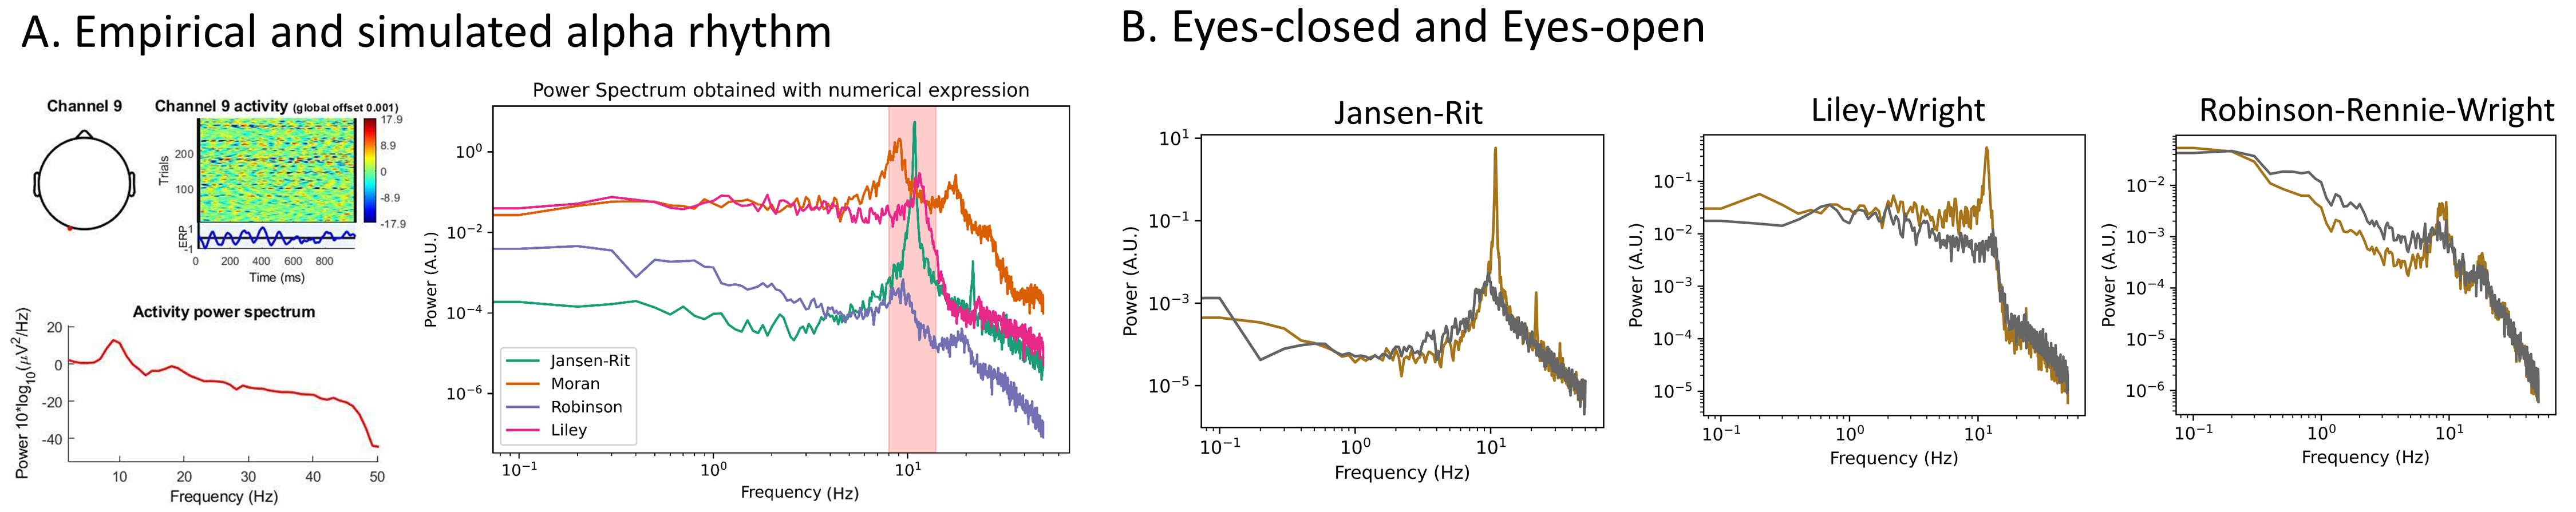
\includegraphics[scale=0.45]{Images/Figure_alpha_short.png} 
    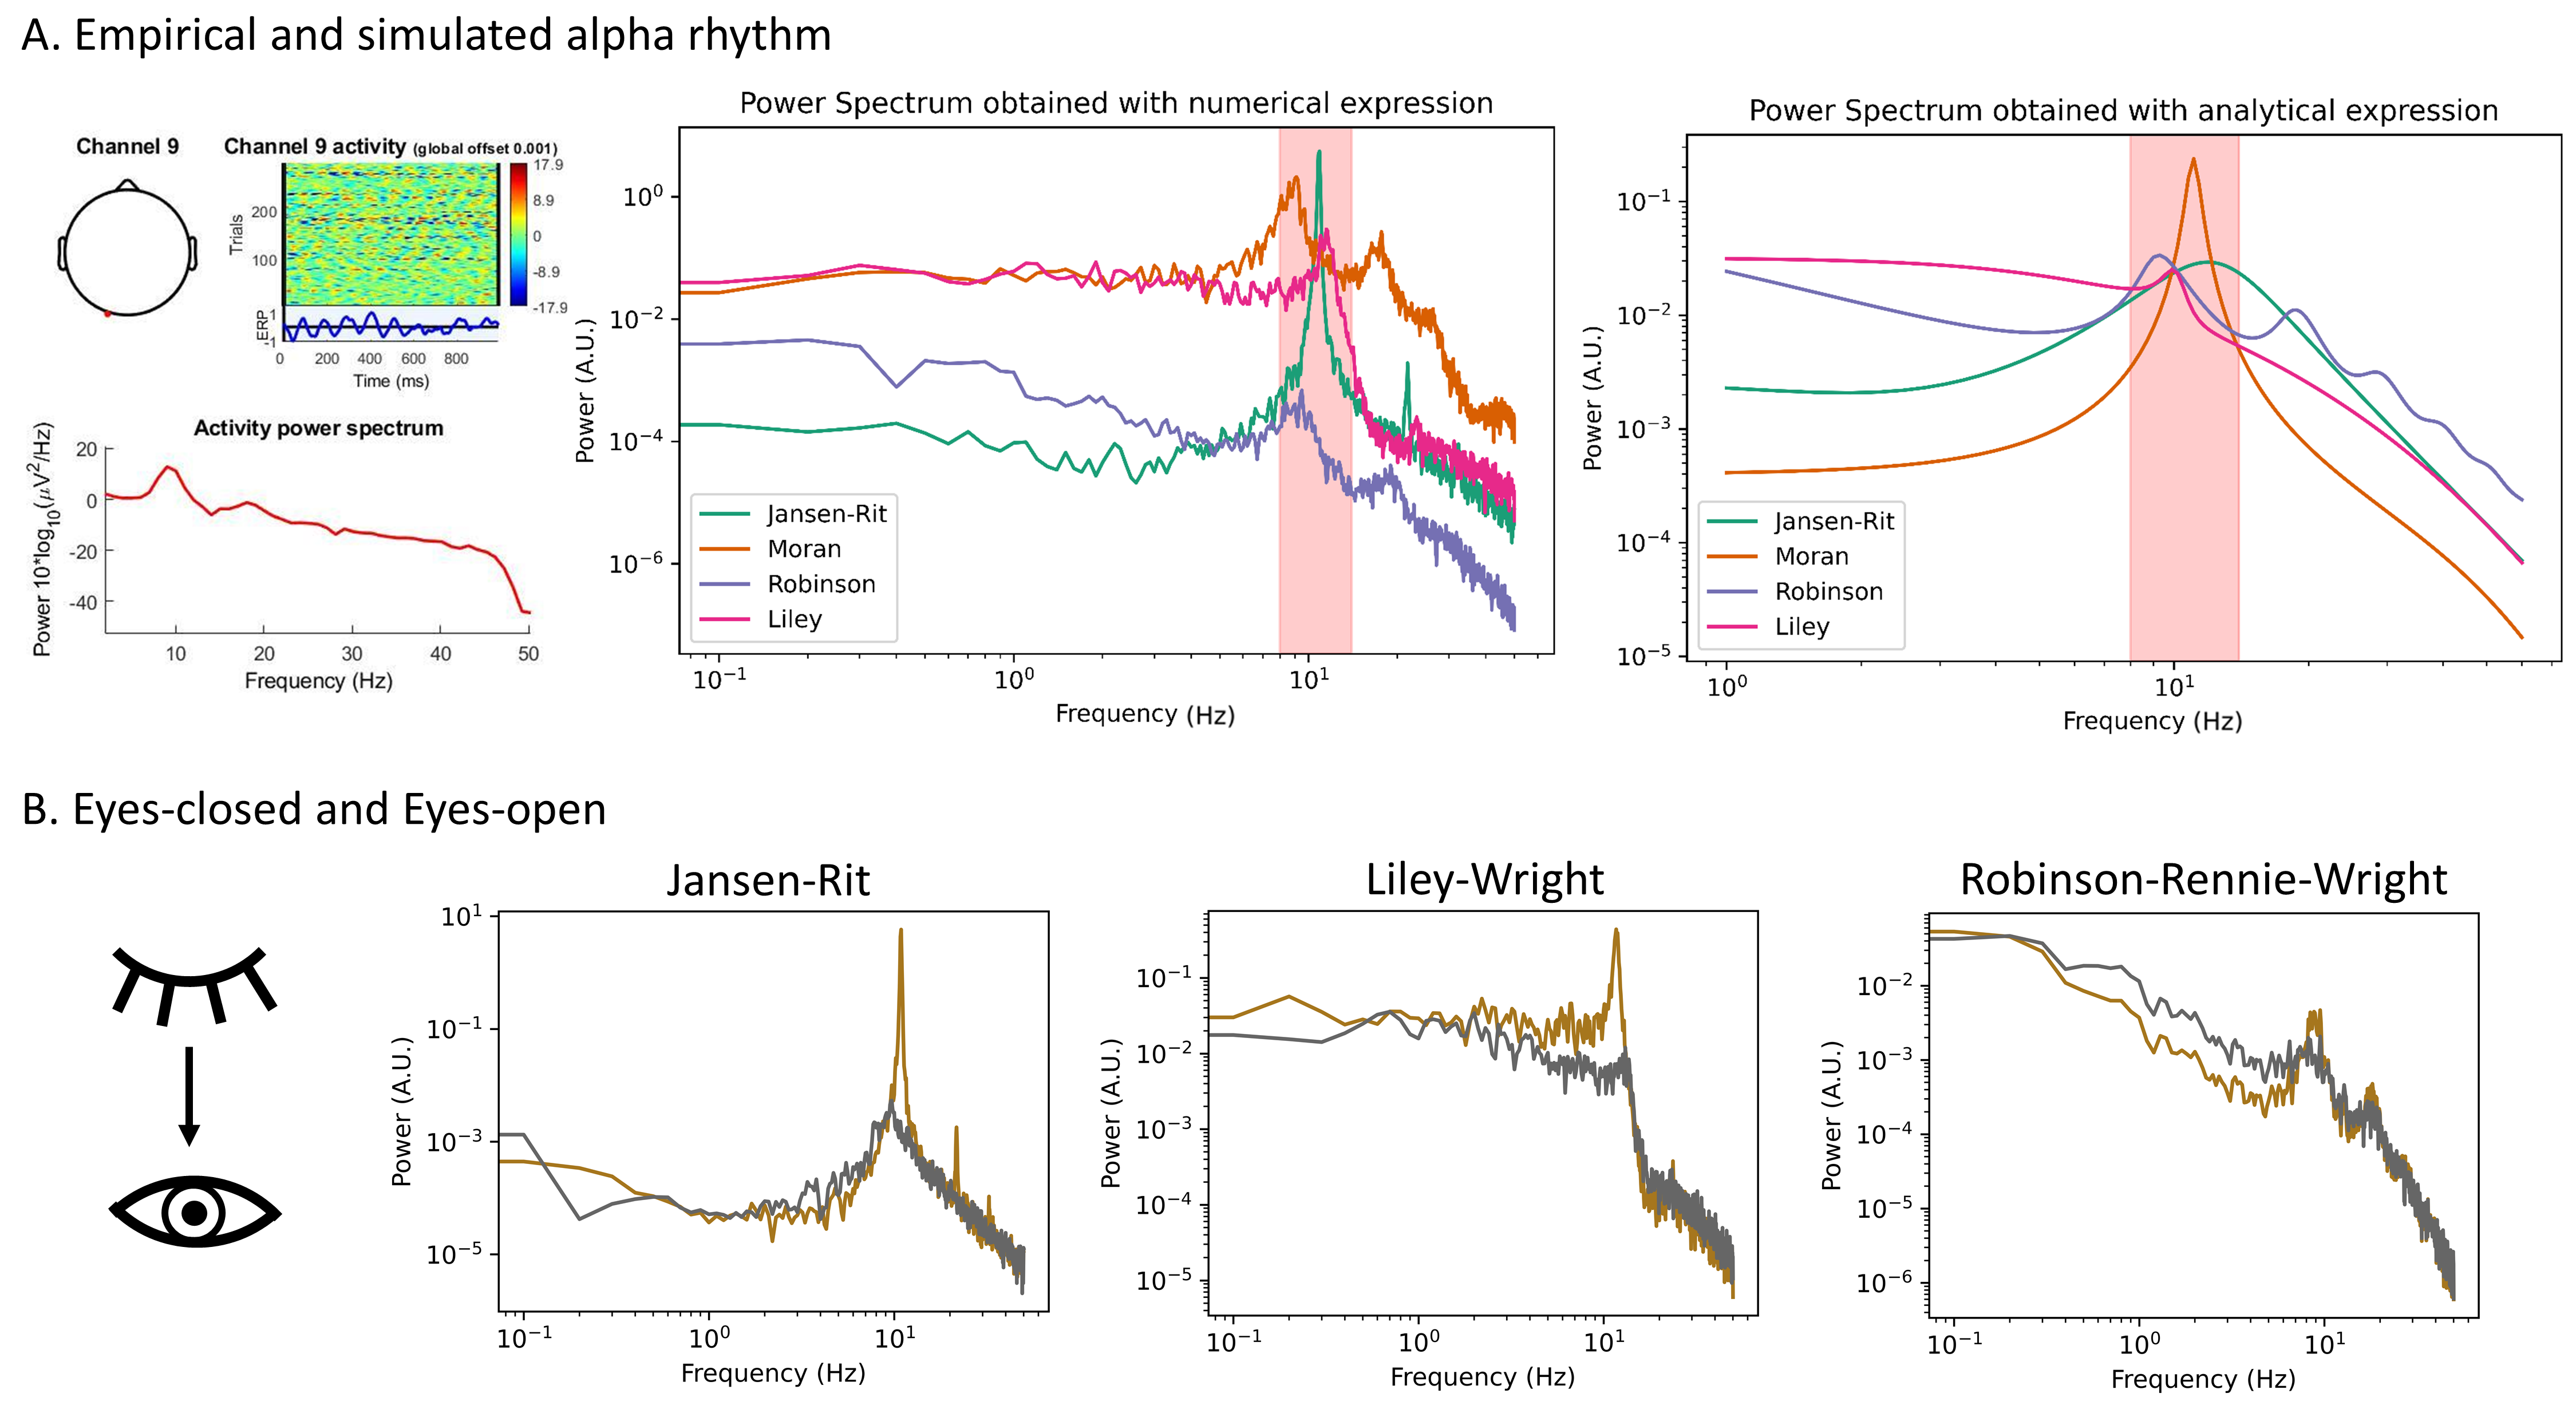
\includegraphics[scale=0.4]  {Images/Figure_alpha_2.png} %0.5
    \caption*{\textbf{Figure 8.   \textit{Simulation results with standard parameter settings to generate characteristic resting state alpha oscillations features}} \textbf{A)} Power spectra with characteristic occipital alpha rhythm from empirical EEG time series (left), from numerical simulation results (middle), and from analytical simulations (right). The red zone in the simulated results corresponds to the alpha range. All models generate an alpha oscillation with variations in specific features (peak frequency, presence of harmonics, 1/f shape). \textbf{B)} Simulation results for EC and EO in JR, LW and RRW. The difference from EC to EO is an attenuation in the amplitude of the alpha rhythm. }
    \label{fig:Alpha_results}
\end{figure}
\vspace{-1cm} 
\paragraph{\textit{1/f scaling}} ~\\
Empirical studies have shown that aperiodic activity (also known as 1/f noise) observed in EEG power spectra following a power-law function could play a functional role in healthy brains and explain disease symptoms. For example, cognitive decline in ageing has been associated with increased 1/f noise (slope) in the power spectrum \citep{voytek2015age}, as well as aperiodic variations in stroke patients \citep{johnston2023spectral}.
The 1/f noise is therefore an important feature of resting state EEG. Visually, the shape of the 1/f curve from RRW closely resembles the empirical 1/f curve (see e.g. \citealp{freeman2003spatial, dehghani2010comparative}). In contrast, this feature is poorly represented by JR, which may be due to the fact that the JR system generates almost a perfect sinusoid, whereas RRW for instance seems to have more aperiodic fluctuations in the EEG time series.\\
Table 1 presents the computed data feature values across all four models. Comparison with the mean empirical EEG result (1.36) shows that 1/f pre-peak values are considerably lower for JR and LW (0.36 and 0.48 respectively), but higher for RRW (1.64). Empirically, lower frequencies (pre-peak) exhibit steeper slopes in frontal areas, but these quantities for the JR and LW models are notably low.
At higher frequencies (1/f post-peak), JR has the steepest slope (4.03), followed by RRW (3.78) then LW (2.46). All three models yield post-peak values above the empirical mean (1.48). Inversely to lower frequencies, empirically these higher frequencies in the 1/f post-peak range tend to have steeper slopes in posterior areas. However, the simulated post-peak values observed are significantly higher than the empirical values provided in \citet{muthukumaraswamy20181}.

\begin{wraptable}{r}{9.5cm}

%\begin{table}[h]  
\footnotesize
%\small
\centering % centering table  
\begin{tabular}{l c c c c} % creating 10 columns  
\hline\hline   
Model & Main fr. & 1/f pre-peak & 1/f post-peak & Harmonics 
\\ 
\hline   
% Entering 1st row  
 JR & 10.8 & 0.39 & 4.04 & Y \\
% Entering 2nd row  
 MDF & 8.8 & 0.10 & 5.50 & Y \\
% Entering 3rd row  
LW & 11.6 & 0.48 & 2.46 & Y \\
% Entering 4th row
RRW & 9.5 & 1.64 & 3.78 & Y \\
\hline\hline % inserts single-line  
Empirical & $\approx$ 10 & 1.36 & 1.48 & Y\\
\hline
\end{tabular}  
\caption*{\textbf{Table 1. \textit{Evaluating Model Performance against Empirical EEG Features}}  To assess the performance of each neural mass model, we estimated its characteristic features, such as the main frequency, slope, and presence of harmonics, and compared them against the corresponding empirical measures obtained from resting state EEG recordings. These features are known to be informative of the underlying neural dynamics that give rise to the EEG signal. By evaluating the agreement between the model-based estimates and the empirical approximations, we can determine the extent to which the model captures the essential aspects of brain activity during rest.}  
%\end{table}  
\end{wraptable}




To summarize, the models demonstrate an underrepresentation of lower frequencies in JR and LW, and an overrepresentation in RRW. They all exhibit considerably steeper slopes for higher frequencies than the empirical average. This discrepancy may arise because the empirical values reflect an average across the cortex, while our models aim to capture the characteristic eyes-closed alpha peak, predominantly observed in the brain's posterior region. Visually, RRW appears to be the most similar to empirical resting state EEG, especially for the representation of 1/f in lower frequencies, which is not accounted for in the other models. Finally, consistent with empirical findings, all models have lower pre-peak 1/f values than post-peak 1/f values during EC, with higher frequencies displaying steeper slopes in posterior areas within the cortex.  % what is found empirically.  
% Although still higher than the range observed empirically even in occipital I think. From the paper: βhf and βlf values obtained from resting eyes-closed data showed considerable variation across the cortex. For the high frequencies (βhf) mean slope was 1.21 (range 0.78–1.45) while for the lower frequencies the mean slope was 0.76 (range = 0.56–0.98). A clear spatial pattern was evident (Fig. 2a and b), such that in the higher frequencies steeper slopes are present in posterior areas whereas for the lower frequencies (βlf) steeper slopes are present in the frontal cortex. 

% If do MDF as well add the results in text

\paragraph{\textit{Eyes open vs. Eyes closed}} ~\\
A defining characteristic of the resting state alpha rhythm in visual areas is that its amplitude is attenuated in EC compared to EO conditions, a phenomenon known as \textit{alpha blocking} \citep{barry2017eeg, adrian1934berger, chapman1962quantitative}. We examined the ability of our surveyed models to reproduce this effect by modifying relevant parameters based on previous research findings. In LW, increasing the external input to the inhibitory cortical population resulted in a reduction of alpha activity, consistent with the intuitive idea that an increase in the amount of incoming visual information is what characterizes the transition from EC to EO \citep{hartoyo2020inferring}. Similar effects were also observed in the JR and MDF models, where an increase in external input led to the alpha blocking. In these cases however, input is (and can only be) delivered to the excitatory rather than the inhibitory neural population. 
%Check not representing input from thalamus
For RRW, we selected a specific parameter set that simulates the EO state based on detailed studies conducted by
\citet{rowe2004estimation}. According to these authors, the transition from the EC to EO state is associated with a decrease in cortico-thalamocortical and intrathalamic gains, accompanied by increased cortical gains and dendritic rate parameters, which together lead to an alpha blocking behavior in RRW. Interestingly, these observations regarding RRW are broadly consistent with the behavior of the three intracortical models: In JR, MDF, and LW, the attenuation of the alpha rhythm is caused by an increase in input representing incoming visual stimuli. In the case of RRW, it is mediated not by a direct input per se, but by a decrease in corticothalamic interactions and an increase in cortical gains. This increase in cortical activity causing alpha blocking in RRW could be considered analogous to the increase in cortical activity caused by greater driving input in JR, MDF, and LW.

In summary, all four models capture key features of empirically observed alpha rhythms, in terms of frequency peaks, harmonics, alpha blocking, and 1/f scaling. %On the last of these, it should be noted that the 1/f exponent values listed in Table 1 for canonical model parameters do not fall within the empirical range as given by \citep{muthukumaraswamy20181}. 
Of the four, RRW is in general notably closer to empirical EEG data in both its 1/f behavior and its harmonics. It is important to acknowledge however that this analysis is based on a specific set of parameters, which can be restrictive given the wide range of parameter combinations that can give rise to the alpha regime. Therefore, further exploration of the parameter space boundaries is crucial to gain a more comprehensive understanding of the emerging behavior and dynamics of the alpha rhythm.  
% Paper for difference between EC and EO empirical https://www.sciencedirect.com/science/article/pii/S1388245707004002?via%3Dihub
%\begin{figure}[H]
 %   \centering
  %  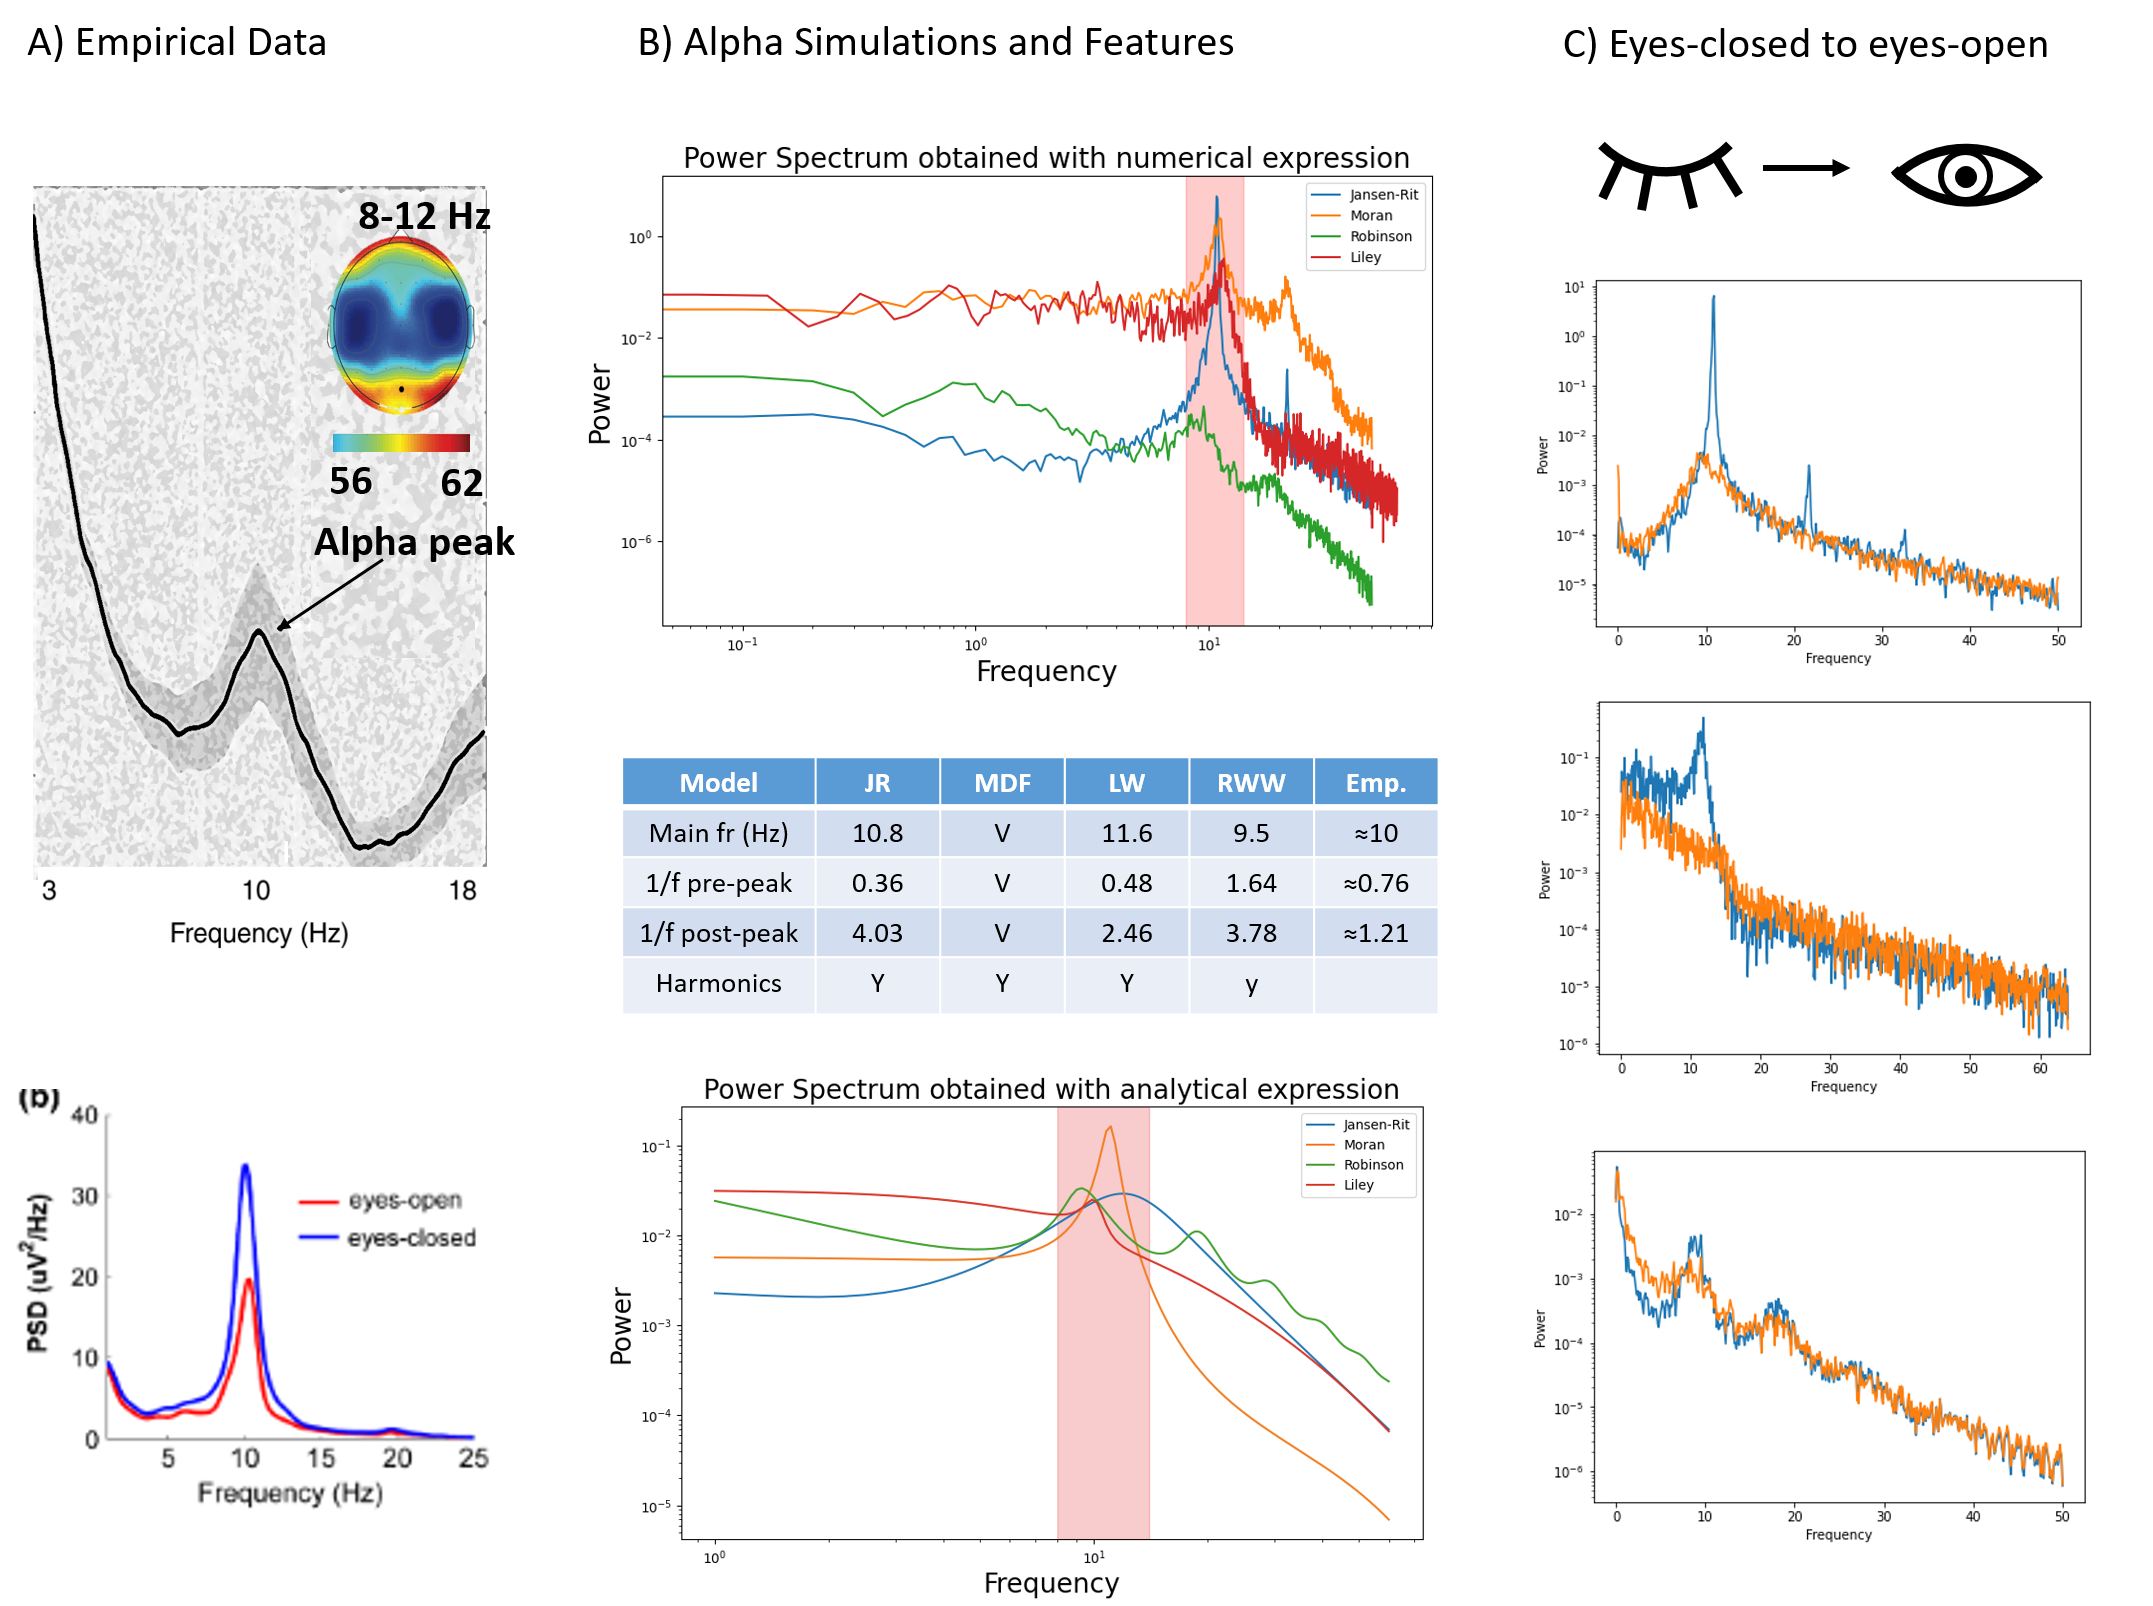
\includegraphics[scale=0.5]{Images/Alpha_all_results.png}
   % \caption*{\textbf{Figure 12.  \textit{Simulations results of each model to reproduce alpha oscillations with numerical (left) and analytical expression (right).}} All model generate alpha oscillations (peak in red zone (8-12Hz). Difference in shape, amplitude and 1/f components}
    %\label{fig:Alpha_results}
%\end{figure}
%TC:ignore

%TC:endignore


\vspace{-\baselineskip} 
%TC:ignore

\vspace{0.5cm}
\subsubsection{Structure of parameter space}
%TC:endignore
Alpha oscillations are generated by non-unique parameter sets, and while there may be quantitative differences in parameter values between models, their qualitative behavior may be similar. Next we explore alpha regime boundaries and the necessary conditions for producing a dominant frequency in the alpha range, as a function of rate constant and connectivity parameters. We also identify any other dynamical regimes that the models may present. Parameters with similar biological interpretations between the models are compared in order to provide a meaningful comparison.  
To ensure consistency, all other parameters are maintained in their standard resting state setting (Tables in S.9).

%\newpage
\paragraph{\textit{Rate constant parameter space dynamics}} ~\\
The JR, MDF and LW models have distinct excitatory and inhibitory impulse responses that are modulated by rate constants ($\tau_{e}$ and $\tau_{i}$). These rate constants reflect collective passive dendritic cable delays and neurotransmitter kinetics associated with fast synaptic activity involving glutamatergic AMPA and GABA receptors \citep{spiegler2012dynamics}. This synaptic filtering is assumed to take a different shape in excitatory than in inhibitory neural populations in most of the four models, with the exception of RRW - where the same rate constant is used for AMPA as for GABA receptors. Previous studies have demonstrated that the manipulation of these rate constants can significantly impact the dominant frequency of oscillations \citep{david2003neural, gast2019pyrates}. In our investigation, we aim to determine whether similar patterns of frequency changes can be observed across the parameter space for all three models.

%TC:ignore
%\begin{wrapfigure}{l}{0.6\textwidth}
\begin{figure}[H]
    \centering
    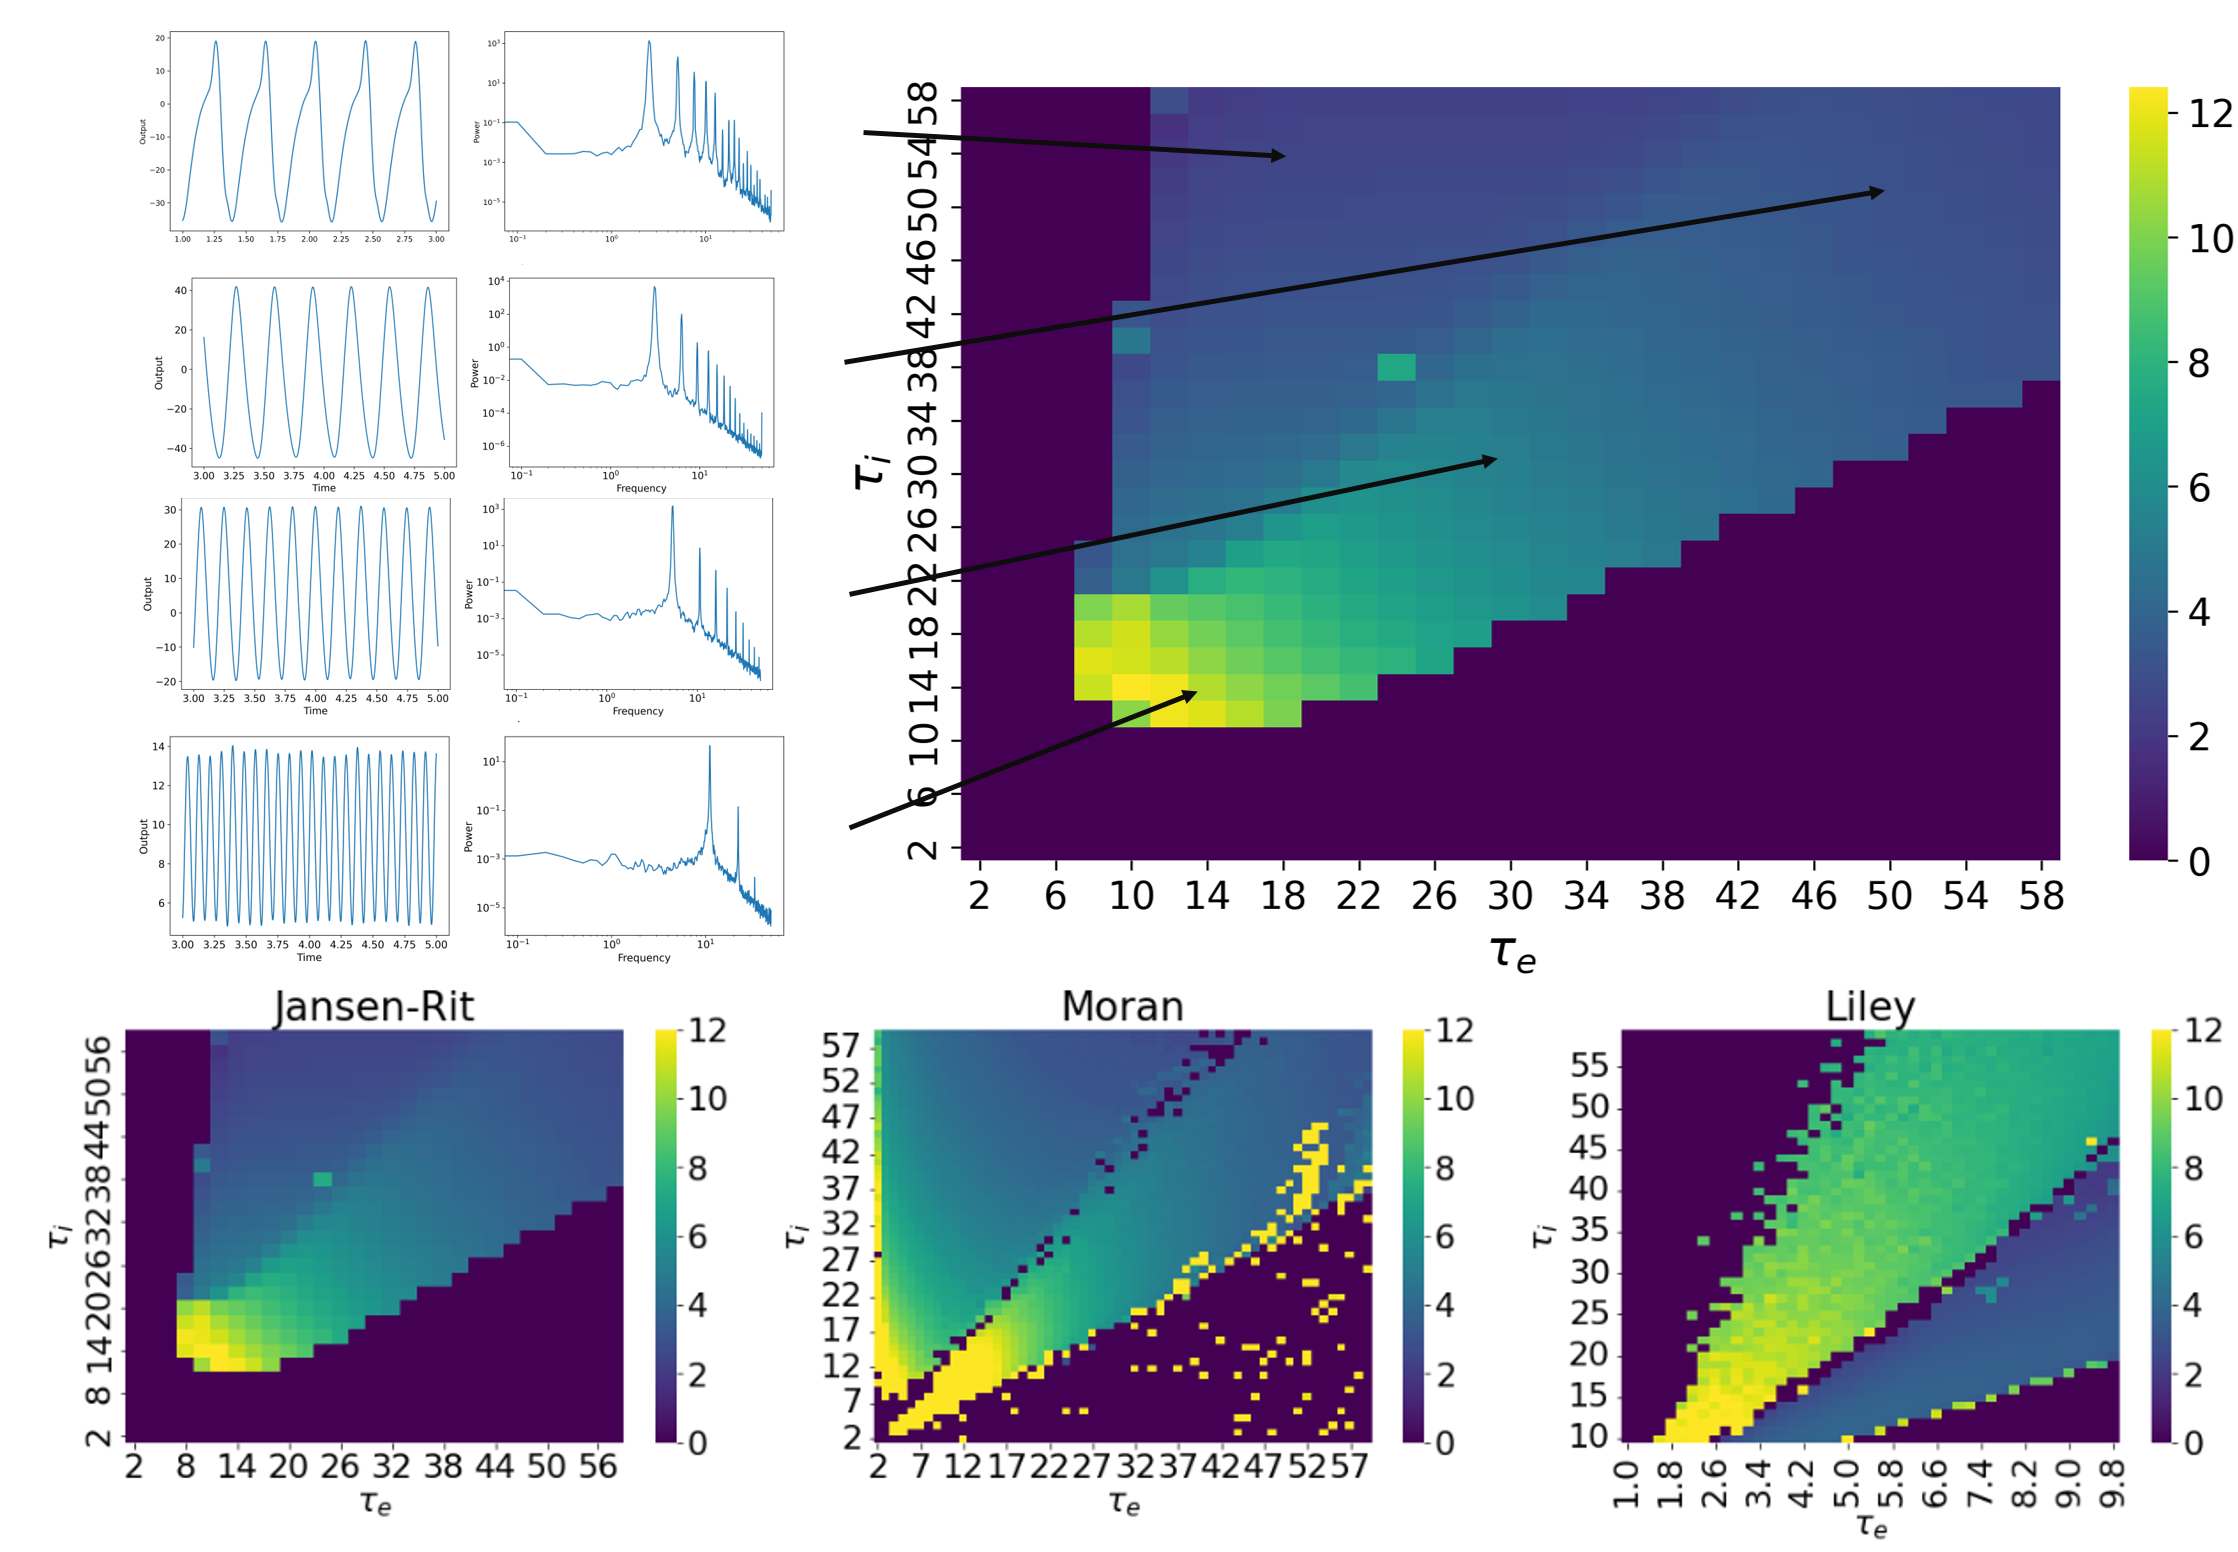
\includegraphics[scale=0.4]{Images/Rate_constant_2.png}%[width=0.6\textwidth]{Images/Rate_constant_4.png}
    \caption*{\textbf{Figure 9. \textit{Effect of rate constants on dominant frequency of oscillation for the JR, MDF, and LW models.}} 
    \textbf{A)} Example time series and power spectra of a set of specific rate constant values to show the slowing in frequency as the values of the excitatory and inhibitory rate constant increase. \textbf{B)} Heatmap presenting the dominant frequency of oscillation as a function of the rate constants of the JR model. \textbf{C)} Three heatmaps for the JR, MDF and LW with the dominant frequency of osicllation as a function of the rate constants. For JR and MDF $\tau_{e}$ and $\tau_{i}$ are varied from 2ms to 60ms. For LW, $\tau_{e}$ changes from 1.72ms to 5ms, and $\tau_{i}$ from 10 to 50ms to generate oscillatory behavior.}
    \label{fig:tau_param_sweep}
\end{figure}
%\end{wrapfigure}
%TC:endignore
Across all models, a consistent trend is observed where the predominant rhythmic frequency decreases with an increase in both rate constants, aligning with previous analyses \citep{david2003neural}. For LW, the range of values for $\tau_e$ and $\tau_i$ differs due to the system's tendency to diverge if $\tau_e$ becomes excessively high compared to $\tau_i$. Due to this, in Fig. 10 we constrain the possible range of values to 1-10 ms for $\tau_e$ and 10-60 ms for $\tau_i$.
% this argument needs to be developed: An explanation for the difference is the presence of an additional neural population in JR and MDF which compensates. Furthermore, this might reflect a more accurate biological model as not any values can be used to represent the rate constants. \\
With a uniform external input, JR has a peak oscillatory frequency of 12.4 Hz, falling within the high alpha / low beta range. MDF can elicit higher beta oscillations with a normal noise input when the rate constants are both small. This suggests that the inclusion of self-inhibitory connections in MDF contributes to generating higher frequency oscillations. Notably, both JR and MDF exhibit a phenomenon known as a `hypersignal' \citep{david2003neural} when $\tau_i$ is considerably higher than $\tau_e$, which is typically associated with lower frequency oscillations. In such cases, the time series does not produce an exact sinusoidal oscillation (Fig. 9). Conversely, if $\tau_e$ becomes too high compared to $\tau_i$, neither model shows oscillatory patterns. This means that a balance needs to be kept in order to maintain a periodic behavior, which can be achieved by keeping the product of $H_{e,i}$ and $\tau_{e,i}$ constant by appropriately adjusting $H_e$ and $H_i$ as $\tau_e$ and $\tau_i$ is modified \citep{david2003neural}. 

In LW, equivalent hypersignal behavior is observed when $\tau_e$ is excessively high compared to $\tau_i$, while in the opposite case of $\tau_i$ higher than $\tau_e$ no oscillatory activity is seen. Furthermore, as shown in Fig. 10, this hypersignal activity occurs above the alpha regime in $\tau_e$ vs $\tau_i$ space for JR and MDF, and below the alpha regime for LW (Fig. 9). What these observations suggest is that the central alpha oscillatory regime in JR and MDF operates in a manner that is intrinsically different to the alpha regime in LW - a question we revisit through the lens of linear stability analyses below. 

As expected, modifying the shape of the synaptic filtering through the rate constants has an influence on the rhythmic behavior of the system. Increasing both rate constants simultaneously leads to a decrease in the frequency of oscillation, as longer delays are then introduced. For example, if a disease affects the propagation of action potentials, it could lead to a decrease in the dominant frequency of oscillation.
In RRW, $\tau_{e}$ and $\tau_{i}$ are assumed to be equal, considering that the difference in rise time between AMPA and GABA-A is negligible and, therefore, the synaptic filtering is the same between excitatory and inhibitory neurons. This assumption could be questioned, however, as changes in rate constants in the other models have been shown to affect the central frequency. 

% Spiegler 2012 for JR: Second, the analysis revealed that the intrinsic temporal ratio β between the inhibitory and excitatory dendritic time constants τi and τe (not their absolute values) determines whether no oscillations, only onetype of oscillation (harmonic or anharmonic) or both types are possible (Fig. 5.4; this confirms the findings of David and Friston [48]). Regarding the system Eqs. (4.1) to (4.7), it is obvious that the dendritic time constants are related to each other by their scaling or respectively the intrinsic temporal ratio β = τe/τi. Hence, the system behavior qualitatively depends only on the intrinsic temporal ratio β and on the extrinsic inputs on both types of interneurons (i. e., EINs and IINs). More specifically, this analysis revealed that for maintaining an oscillatory regime, it is essential to keep the ratio β ≤ 5 (see Fig. 5.6).


\paragraph{\textit{Connection Strength}} ~\\
The strength of connections between neural populations plays a role in facilitating communication, and thus when the strength of these connections is appropriately balanced, it enables coordinated neural activity, leading to the generation of brain rhythms. Even though on the face of it the neural populations included in the four models differ quite considerably, they all exhibit at least one common element - a principal excitatory-inhibitory ($E - I$) loop. The ratio of synaptic weights within that loop relates closely to the concept of `E/I balance', a widely studied physiological phenomenon that has garnered significant attention in neuroscience in recent years \citep{meisel2017decline, zhou2018synaptic, sohal2019excitation, murray2014linking}. We explored the impact of connectivity parameters on the dominant frequency of oscillation. To maintain conciseness, we exclude the connectivity parameter spaces of MDF in this section, since the patterns observed are very similar between JR and MDF, with the distinction that MDF tends to generate higher frequencies of oscillation for the same set of parameter values. A comprehensive summary of the comparison between JR and MDF can be found in S.6. Additionally, S.7 includes a 4D parameter analysis for JR, encompassing all model connectivities.

JR's E-I interaction is represented by the connectivity strength between pyramidal cells and inhibitory interneurons. Since LW is only composed of one excitatory and one inhibitory neural population, the parameters of interest are the two synaptic weights connecting the two populations. Finally, for RRW, the reticular nucleus inhibits the relay nuclei and is considered the inhibitory population of the model. In this context, we consider the relay nuclei as having a central role and can be compared to the pyramidal cells in JR, as they are connected to all other populations. The excitatory-inhibitory interaction explored is then within the thalamus between the relay nuclei and the reticular nucleus. It should be noted that this interaction is not an isolated loop, because it is embedded within the larger cortex-reticular nucleus-relay nuclei loop, and so is also affected by the activity from the cortex. However, for simplicity, our focus is on the E-I interaction between the two thalamic populations.


%The comparison between JR and MDF is summarized in the Appendix B. \\

%TC:ignore
\begin{figure}[H]
    \centering
    %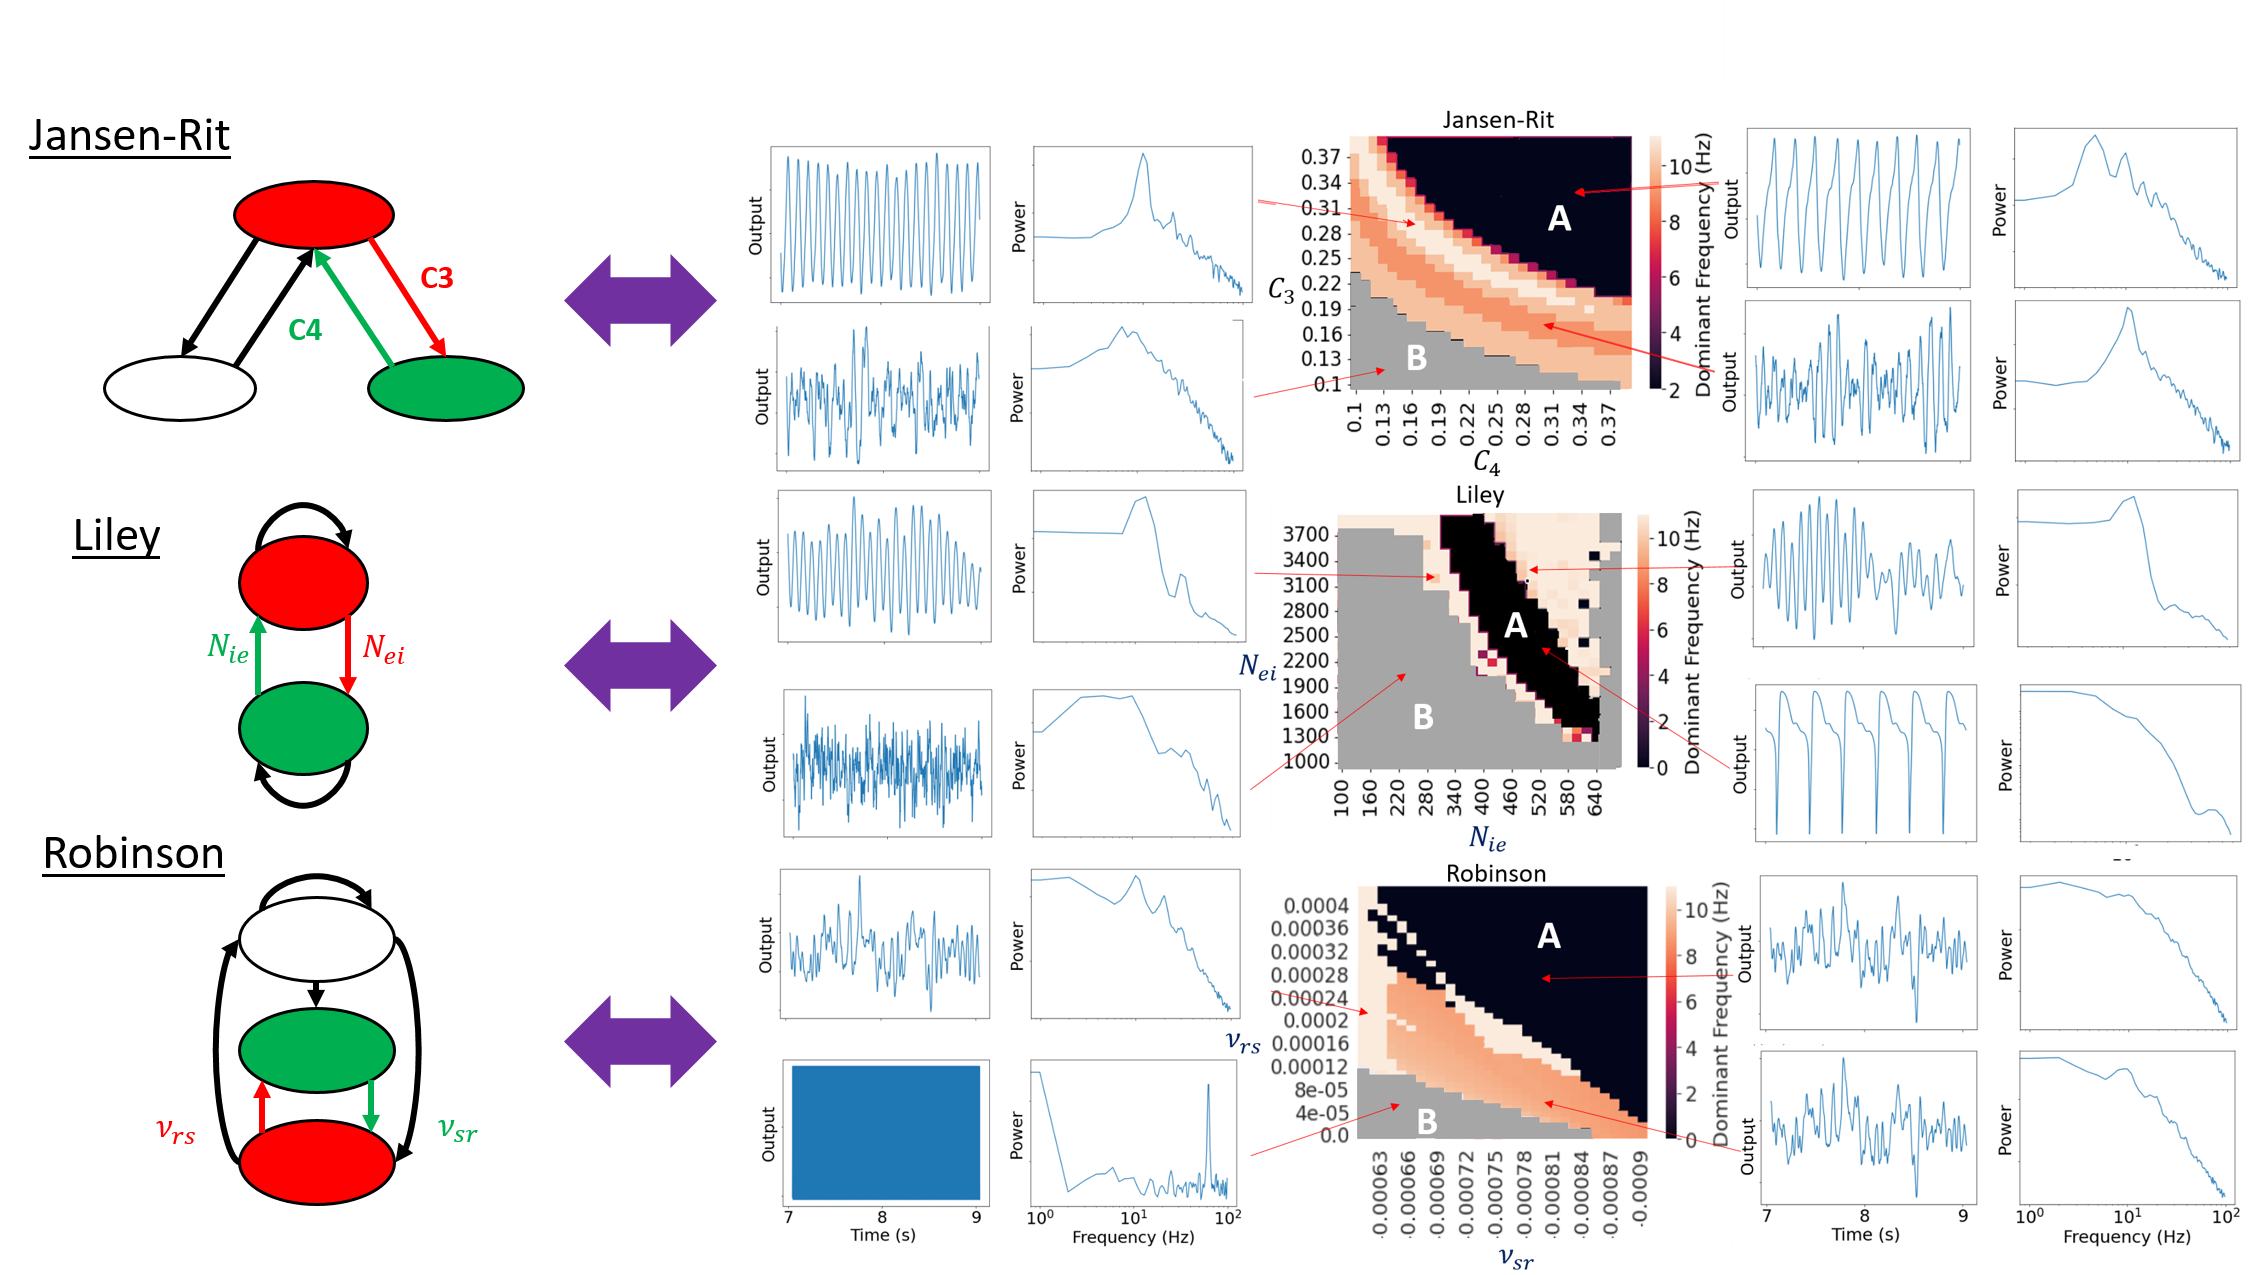
\includegraphics[scale=0.49]{Images/Connectivity_final.png}
    %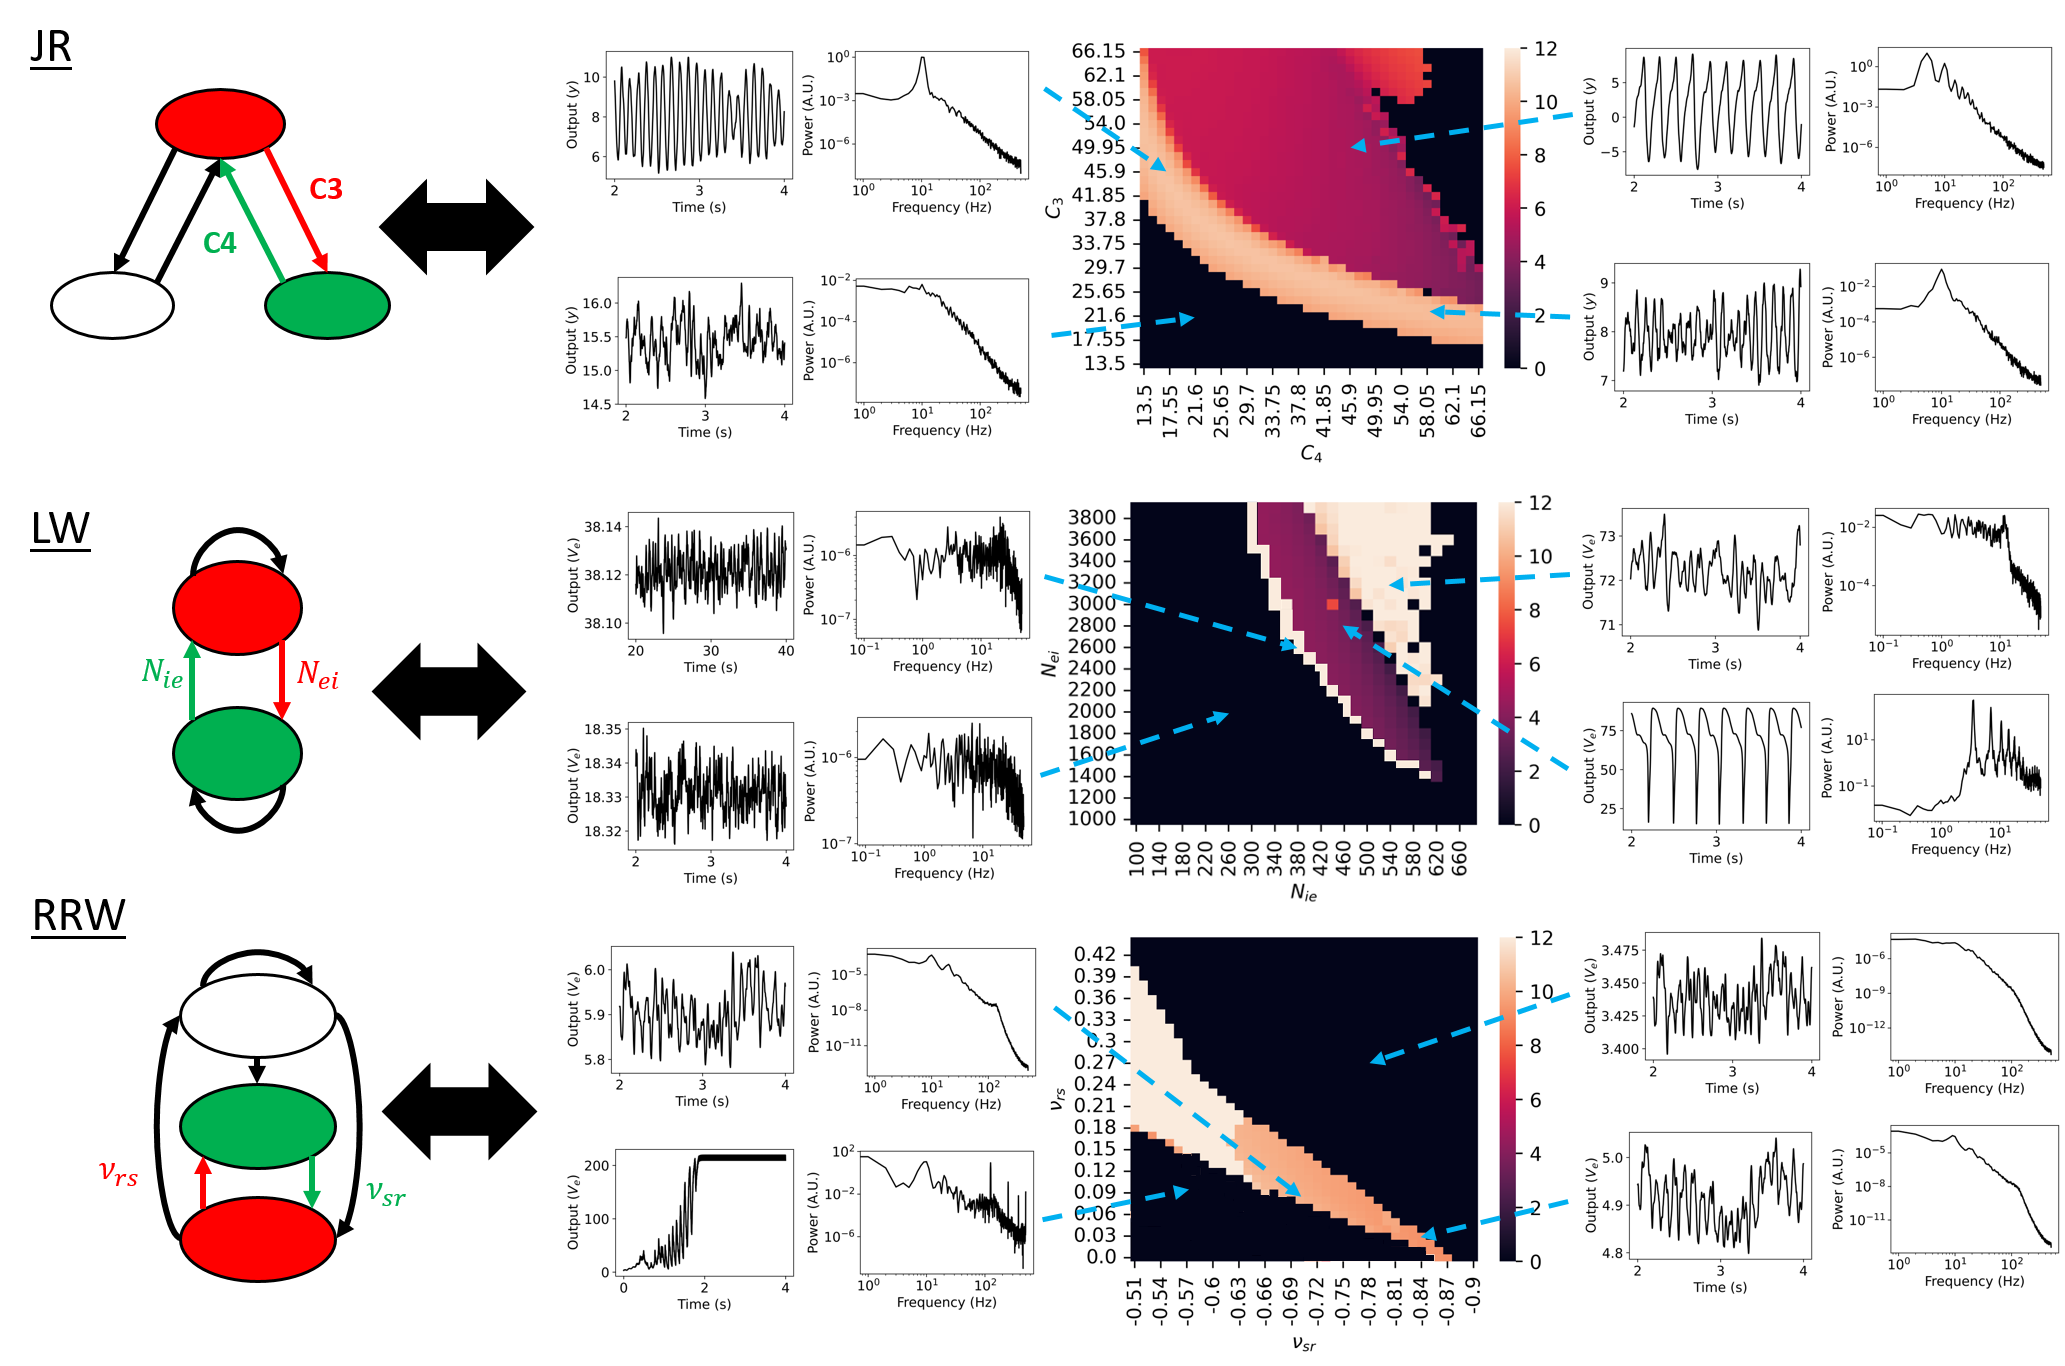
\includegraphics[width=\linewidth]{Images/Connectivity_3.png}
    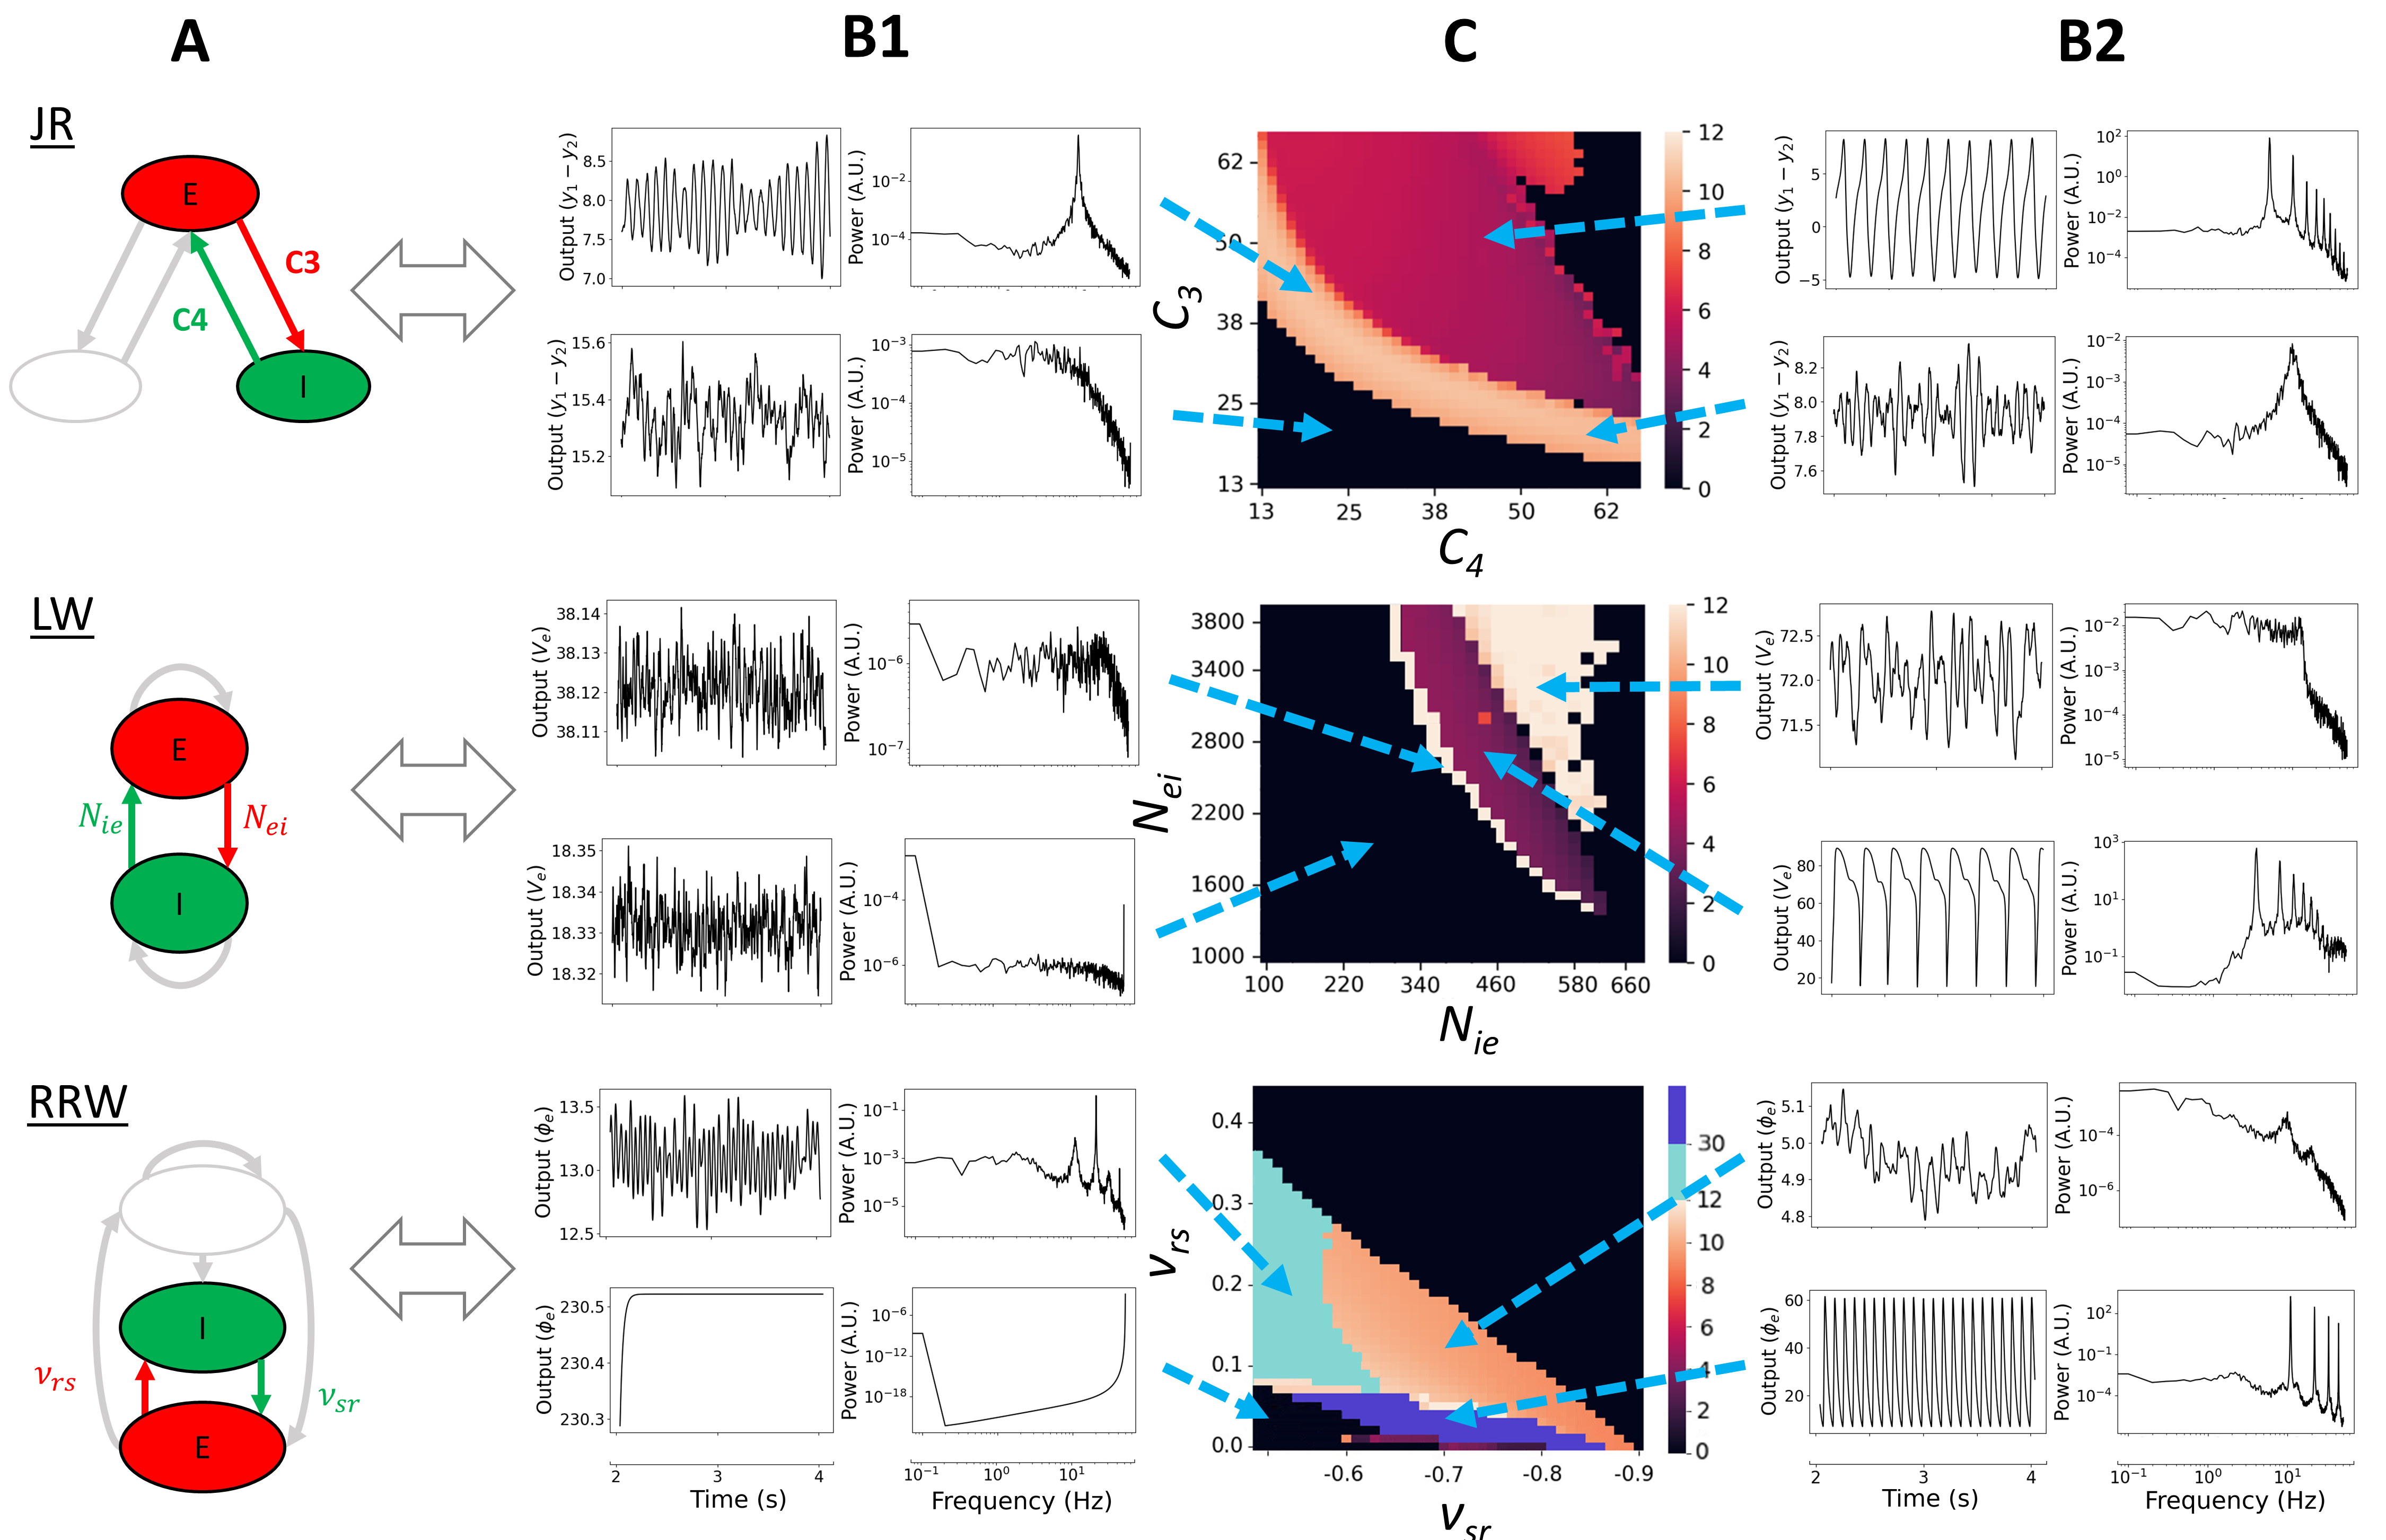
\includegraphics[width=\linewidth]{Images/Connectivity_5.png}
    \caption*{\textbf{Figure 10.  \textit{Frequency of oscillation parameter spaces as a function of E-I connectivities}} \textbf{A)} Schematic of the models with their principal E-I loop highlighted. These are the parameters that are going to be varied. \textbf{B1 and B2)} Time series and corresponding power spectra for specific combinations of E-I, showing different dynamics. \textbf{C)} Heatmaps presenting the dominant frequency of oscillation as a function of E-I connectivity. The dark region presents non-oscillatory or non-physiological time series. JR and LW have a clearly defined regime of lower frequency of oscillations being generated (purple and red region), whereas RRW quickly tends to produce signals of lower amplitude, or higher frequency of oscillations. In RRW, the dark blue regime indicates that the system is still oscillating but at a higher amplitude and higher frequency as the system is starting to explode. In the light blue regime, the dominant frequency of oscillation is in the beta regime. In the three models, white or orange areas correspond to alpha or higher oscillations.} \label{fig:All_EI_Together}
\end{figure}
\vspace{-\baselineskip} 
%TC:endignore

After exploring various parameter ranges, we identified specific values that produced distinct behaviors for each model, and focused on these dynamic regimes. Results of these analyses are shown in Fig. 10. As can be seen in the heatmaps, we observe an inverse diagonal relationship between E-I connectivity and the parameter regime giving rise to alpha frequency oscillations in all three models. This illustrates the fact that it is the total amount of E-I connectivity, or the total E-I gain, that defines the presence of alpha rhythm in these models. A second common feature across all three models is that if the excitatory or the inhibitory connectivity is too low, non-physiological results are obtained. These include time series with either very low amplitude or very high frequency (dark region in Fig. 10 panel D), highlighting the importance of the interaction between these two populations for the generation of rich neural dynamics. 

The relationship between $C_{3}$ ($P \rightarrow I$) and $C_{4}$ ($I \rightarrow P$) in JR needed to generate alpha oscillations follows an exponentially decaying shape. A similar correspondence is observed in LW, although with a narrower range of possibilities due to model constraints. LW also shows a steeper slope, indicating a stronger effect on oscillatory frequency of the input from GABA interneurons ($N_{ie}$) than the input to GABA interneurons ($N_{ei}$). Both the JR and LW models generate lower frequency oscillations, corresponding to the hypersignal regime, as observed in the analysis of rate constant parameter space (purple color in the JR and LW heatmaps in Fig. 10 C, rows 1 and 2). In the LW, if the connectivities are increased beyond this regime, predominantly alpha-frequency activity is generated (triangular white zone above the purple region), which corresponds to the dynamics observed with standard connectivity parameter values. To better understand this difference, a local stability analysis was performed to define the fixed points of the JR and LW models, and expand on their dynamical characteristics (Fig. 11). In the case of JR, the colored alpha regime presents unstable fixed points that continue into the hypersignal regime. These oscillations are due to an Andronov-Hopf bifurcation, wherein the system enters a limit cycle that changes shape over time (Fig. 11, A1, A2). In LW, an Andronov-Hopf bifurcation also occurs, explaining the hypersignal and some higher frequencies on the left hand side of the lower frequency region (Fig. 11, B1 and B2), including alpha. However, the alpha regime in LW generated with standard parameter values lies within the space of stable fixed points (Fig. 11, star in B2), which corresponds to the triangular white regime in the LW heatmap (Fig. 10, C LW). This implies a separate emergent mechanism of alpha rhythm in LW that is distinct from the emergence of a limit cycle that is seen in JR. The generated alpha in this setting is noise-driven, since without noise the system becomes a damped oscillator (due to its having complex eigenvalues with negative real part), and eventually reaches the fixed point. The noise fluctuations repeatedly push the system away from its fixed point at the frequency of alpha, but it tends to stay around that stable point instead of reaching a self-sustaining limit cycle oscillation. This is shown in S.4, which includes the stability analysis of JR and LW under conditions of low or no noise input. Additionally, Fig. 11 depicts the phase plane, showing only the outputs of the pyramidal cells and inhibitory interneurons. In S.5, we extend this by presenting the phase plane in 3D, incorporating the activity of excitatory interneurons as well. 
%This finding is consistent with the observations of previous authors that LW can produce different types of alpha rhythms that are not continuous in parameter space \citep{liley2014neural}. %check where in the source exactly. 
The stability analysis presented here corroborates the idea that the standard alpha rhythms generated by the LW and JR models constitute two mechanisms that are both physiologically and mathematically distinct. This is consistent with the rate constant and connectivity parameter space results as in the rate constant result, we could identify the hypersignal regime above the alpha regime for JR but below for LW, which is also seen in the connectivity parameter space result.

%We also conducted an investigation into the effect of low noise in JR (Fig. 12, 2a and 2b). This analysis revealed that while the shape of the fixed points curve changed, an Andronov-Hopf bifurcation still occurred, and limit cycle trajectories are still present as can be seen in Fig. 12, 2b (star example).
We note that, similarly to the rate constants analysis, $C_{3}$ ($P \rightarrow I$) and $C_{4}$ ($I \rightarrow P$) in JR have ranges of equal values, whereas in LW $N_{ei}$ is significantly larger than $N_{ie}$. This discrepancy can be attributed to the fact that in JR there is a higher level of excitatory interactivity, due to the additional connections between pyramidal cells and excitatory interneurons ($C_{1}$ ($P \rightarrow E$) and $C_{2}$ ($I \rightarrow P$)), which also have higher values than pyramidal-inhibitory interneurons. 

As can be seen in Fig. 10, the connectivity values of RRW are of a much smaller range compared to JR and LW, because they represent the connection strength (mean number of synapses times the strength of the response to a unit signal) in $mV$s rather than the number of synapses between neural populations. Extensive explorations of parameter spaces for this model have been conducted by several authors previously, often using a mathematically simpler reduced version that summarizes connection strengths across aggregated corticocortical, corticothalamic, and intrathalamic loops \citep{roberts2012corticothalamic, abeysuriya2015physiologically}. A notable feature of these analyses using the reduced RRW model is the finding that the parameters most strongly influencing the transition from an alpha-frequency regime to lower frequency dynamics are predominantly associated with the corticothalamic loop. The values of these corticothalamic loop parameters in turn determine the effect of variation in intrathalamic loop parameters on the dynamics. In our study, employing parameter sets corresponding to EC conditions, we observed that increasing the intrathalamic connectivities simultaneously led to a decrease in the amplitude of the alpha peak, accompanied by a slight shift in the central frequency. When the change in $\nu_{sr}$ and $\nu_{rs}$ are sufficiently high, then the alpha peak disappears, which corresponds to the dark colored upper right corner of Fig. 10, C row 3. Interestingly, similarly to the JR and LW models within the analogous parameter range, we observed in RRW an inverse relationship between $\nu_{sr}$ and $\nu_{rs}$. However, as $\nu_{rs}$ becomes more negative and $\nu_{rs}$ smaller, the alpha regime reduces. Frequency increases as well as the oscillatory regime as $\nu_{rs}$ becomes more positive. When $-\nu_{rs}$ is smaller than 0.6 we still have alpha oscillations, but there is a dominant peak in the beta range (around 20Hz) seen in B1 row 3 for RRW (light blue region). Finally, if $\nu_{rs}$ is below 0.09 approximately the system starts to explode, resulting in either higher amplitude and frequency oscillations (B2 row 3, dark blue region) or in a continuous very high amplitude value that are not physiologically accurate (B1 row 3, dark region). It seems that $\nu_{sr}$ has an effect on the frequency of the alpha peak which correlates with previous analysis that suggested the importance of corticothalamic interactions as $\nu_{sr}$ is part of the cortico-reticular-relay nuclei circuit. Adjusting $\nu_{rs}$ is key in order to have an oscillatory behavior in the system emphasizing the E-I balance reflected in the other two models. However, due to the numerous connections within the model, the thalamus is probably not the sole connectivity parameter capable of having an effect on the frequency of alpha. 

%This solidifies the importance of corticothalamic interactions in shifting the dominant frequency away from the alpha range. In this initial condition, the thalamus alone does not result in frequency changes, and cortical activity needs to be modulated as well.  We further expanded the parameter range to examine if this relationship continued, and the results indicated an expansion of the oscillatory regime with the generation of higher-frequency rhythms.\
%Ha and expansion of the regime with Robinson model in appendix?.
In summary, through our exploration of E-I connectivity parameter spaces in the preceding pages and in Figs. 9-11, we have demonstrated that the emergence of alpha oscillations in numerical simulations with the JR, MDF, LW, and RRW models requires the neural circuit in question to reach and maintain a sufficient level of E-I gain, whilst also not exceeding a certain threshold amount. This finding emphasizes the importance of achieving a balance between excitatory and inhibitory activity and connectivity, as alterations in this balance can lead to pathological and/or non-physiological oscillatory patterns. The connectivity parameter space results we have shown indicate, in a mathematically explicit fashion, how dysregulation of synaptic connectivity may contribute to abnormal brain activity. Furthermore, in LW, we observed that the dynamics of the model are more strongly influenced by inhibitory connectivity ($N_{ie}$) than by excitatory connectivity ($N_{ei}$). This suggests that an imbalance in the E-I ratio is more likely to be affected by the number or strength of synapses originating from GABAergic interneurons than glutamatergic ones, highlighting the significance of inhibitory interneurons and their synaptic connections in shaping the overall dynamics of LW.
Our stability analyses showed that there are distinct mechanisms underlying alpha oscillations in JR and LW. In our analyses of RRW, the intrathalamic loop was seen to primarily modulate the amplitude of the alpha peak, with little influence on the dominant frequency of oscillation. Thus, in RRW, the dominant frequency of oscillation and the overall dynamics are predominantly modulated by the corticothalamic loop, underscoring the significance of interactions between cortex and thalamus in driving alpha rhythms according to this theory. The narrow range of parameter values leading to alpha oscillations in RRW suggests strong interdependencies among the parameters, which need to be carefully adjusted collectively to maintain oscillatory behavior and clearly detectable spectral peaks in model simulations.

% Note to self: make sure this correlates with what we have
% Spiegler : For the standard Jansen and Rit parameters [54] (also see Table 3.3) their frequency is relatively insensitive with respect to the level of extrinsic input, and ranges between 0 Hz and 80 Hz, depending on the applied intrinsic temporal ratio (as justified in Section 5.1.1), or the dendritic time constants (see Fig. 5.8). For noisy  input, this results in waxing and waning harmonic oscillations of relatively stable frequency. This pattern is compatible with typical brain rhythms, such as the alpha rhythm or sleep spindles. Third, global bifurcations, for example of Shil’nikov type, give rise to homoclinic LCs appearing suddenly at high amplitude and low frequency. They are generally not harmonic, but have a spike-like appearance (anharmonic oscillation). Their frequency depends a great deal on the input levels. Hence, if the PCs receive fluctuating input, the intervals between the wave peaks (or spikes) are variable. These phenomena are compatible with the hallmark of epileptic seizures (i. e., suddenly occurring, irregular spiking patterns (see, for example, [64, 65, 76–78]). It should be noted that Shil’nikov’s bifurcations were also related to "spike-wave" behavior in more theoretical models on MEG and EEG (e. g., [258]). Indeed, this relationship has been also identified in others experimental analysis of using embedding methods (e. g., [261]).





%\begin{figure}[H]
 %   \centering
  %  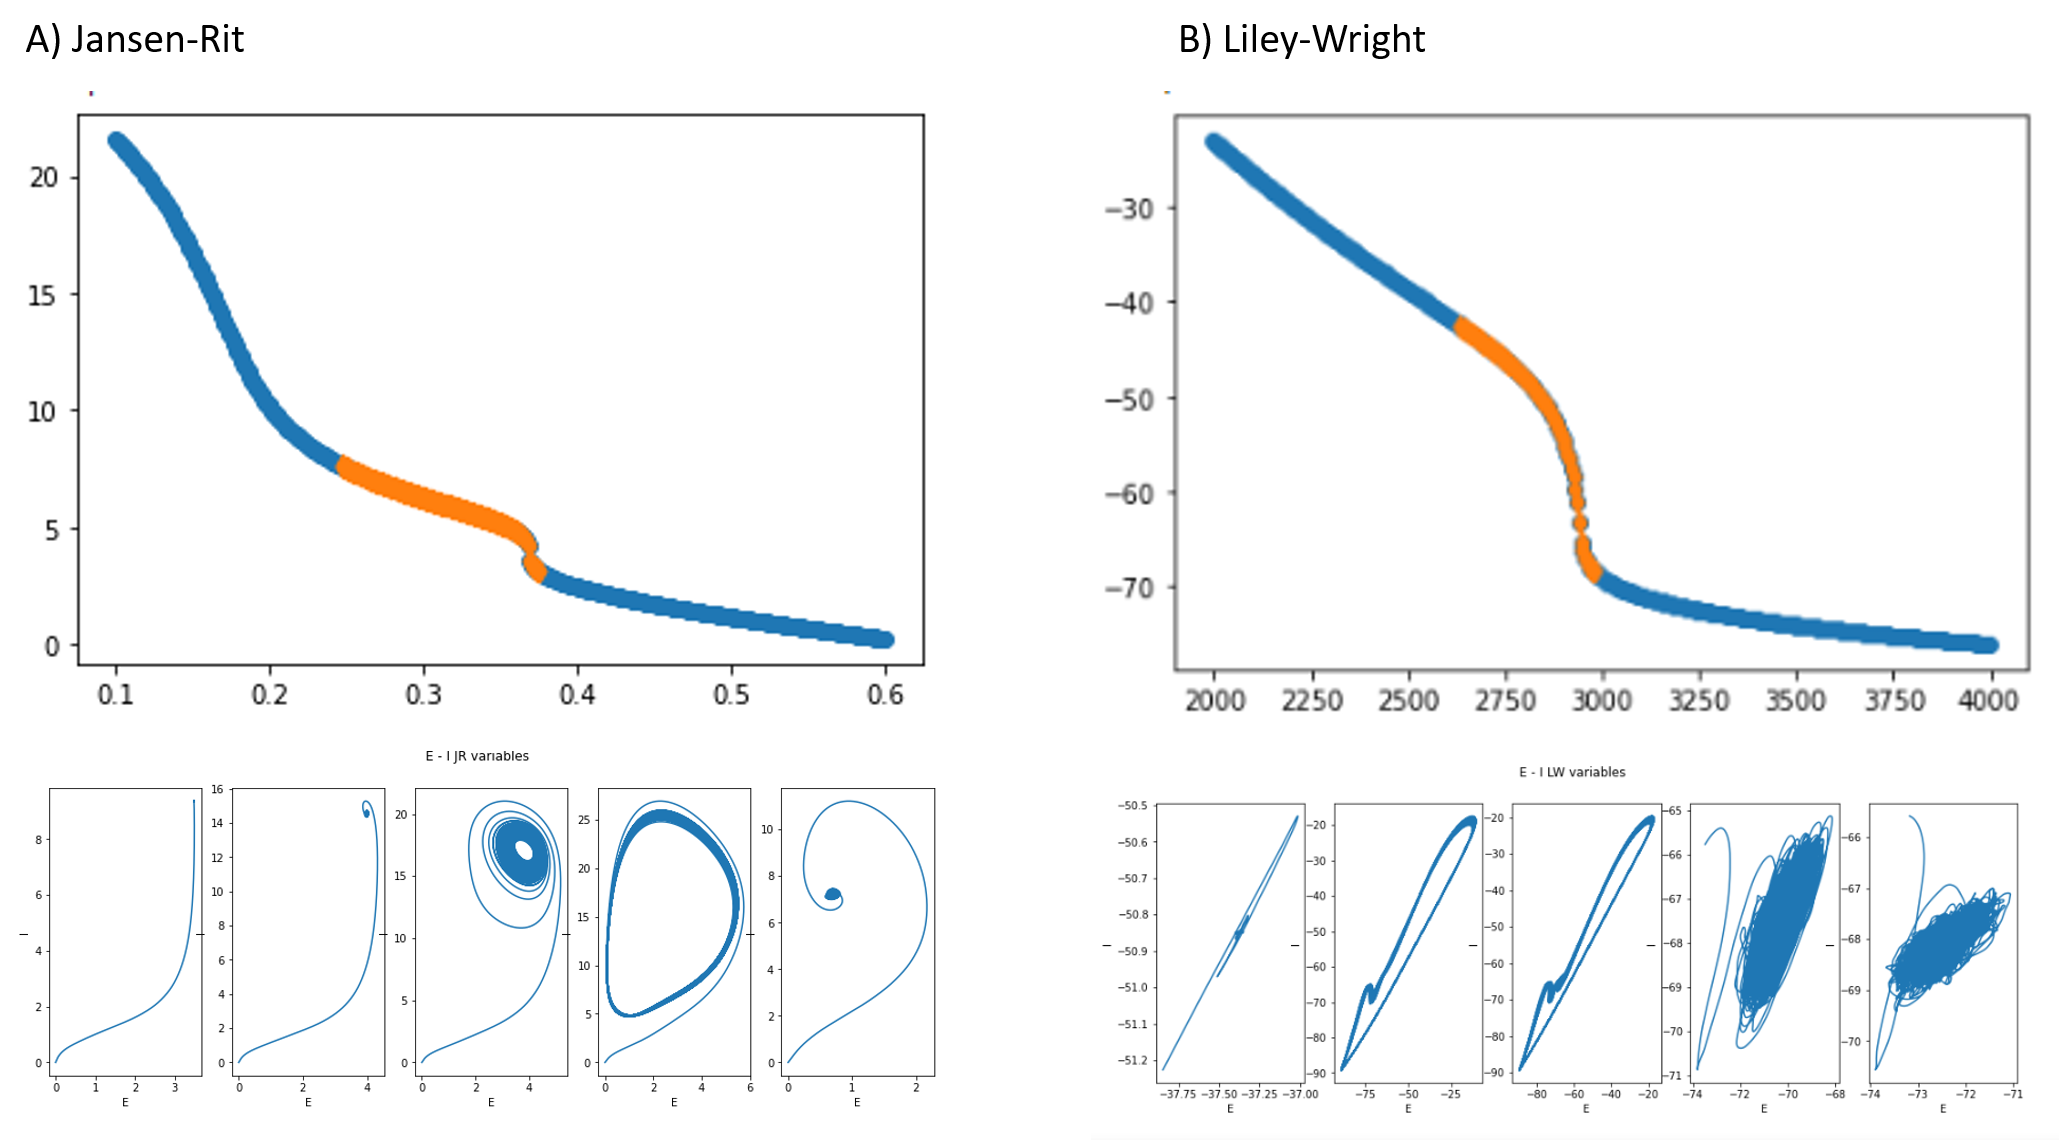
\includegraphics[scale=0.49]{Images/bifurcation_trest.png}
   % \caption*{\textbf{Figure [insert].  \textit{Fixed points and phase planes of JR and LW}} more detailed explanation} \label{fig:Fixed_points}
%\end{figure}
%TC:ignore
\begin{figure}[H]
    \centering
    %\hspace*{-2cm}
    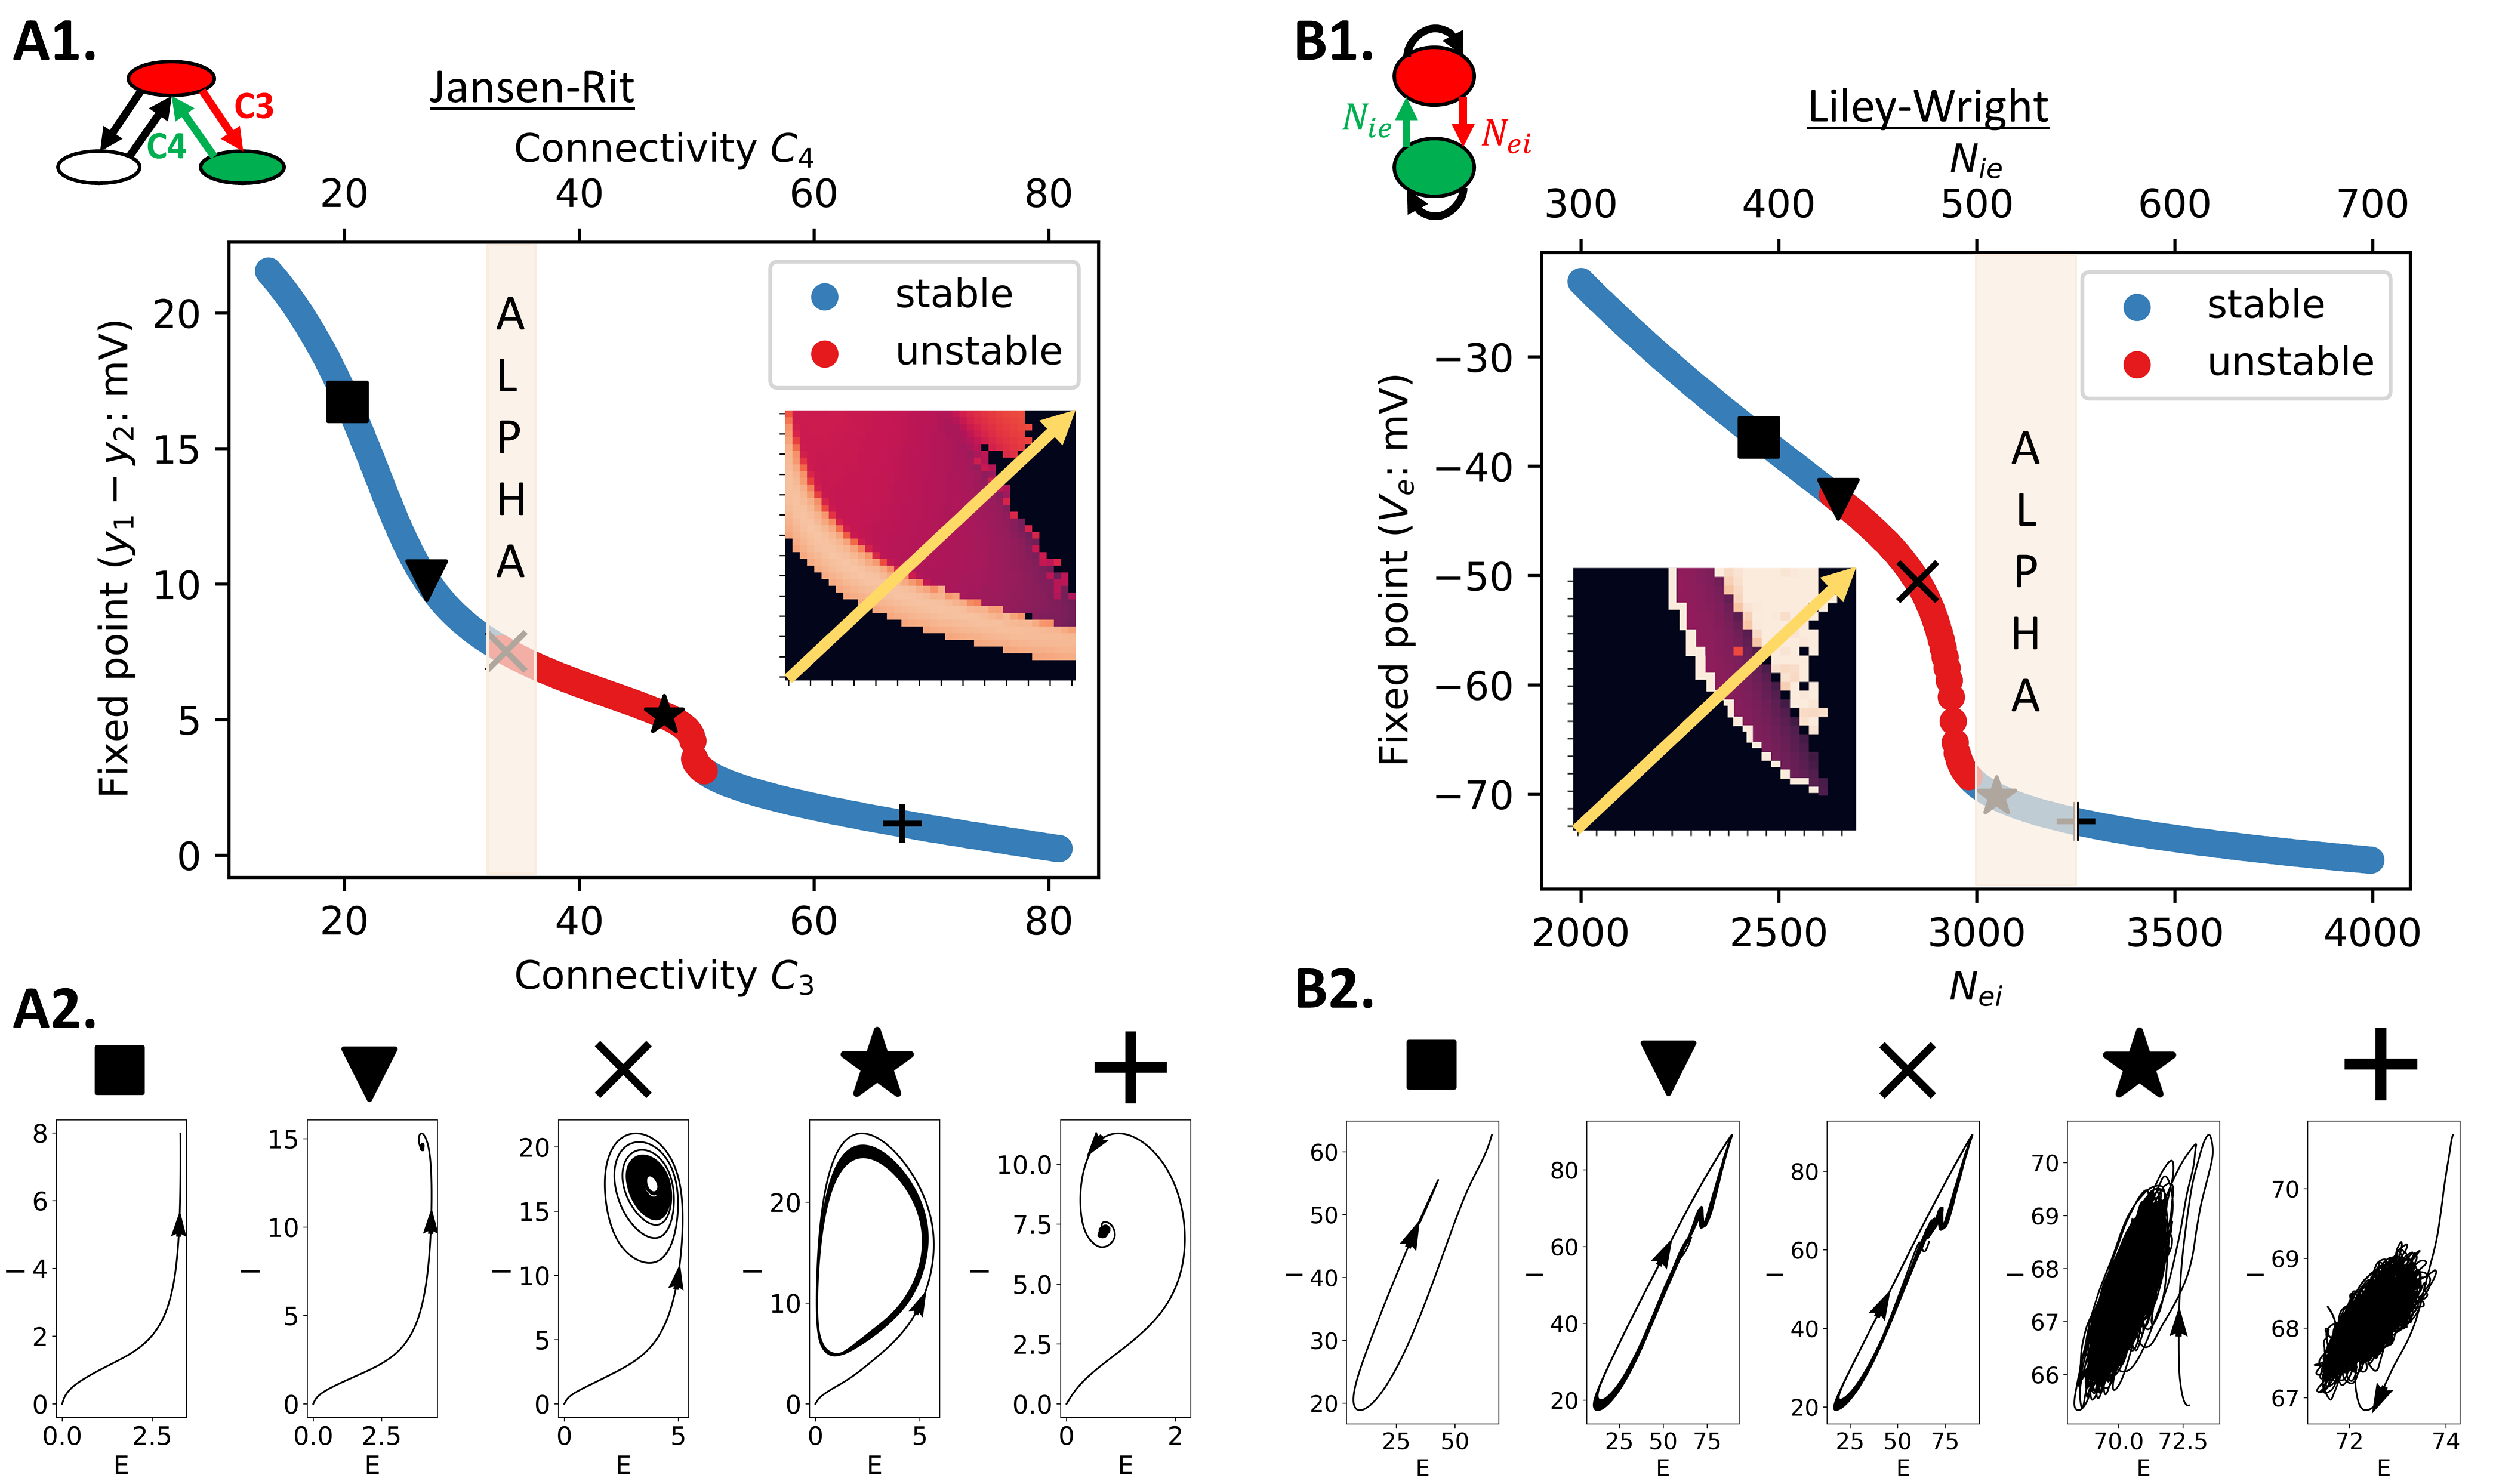
\includegraphics[scale=0.4]{Images/Stability_noise_short.png}
    %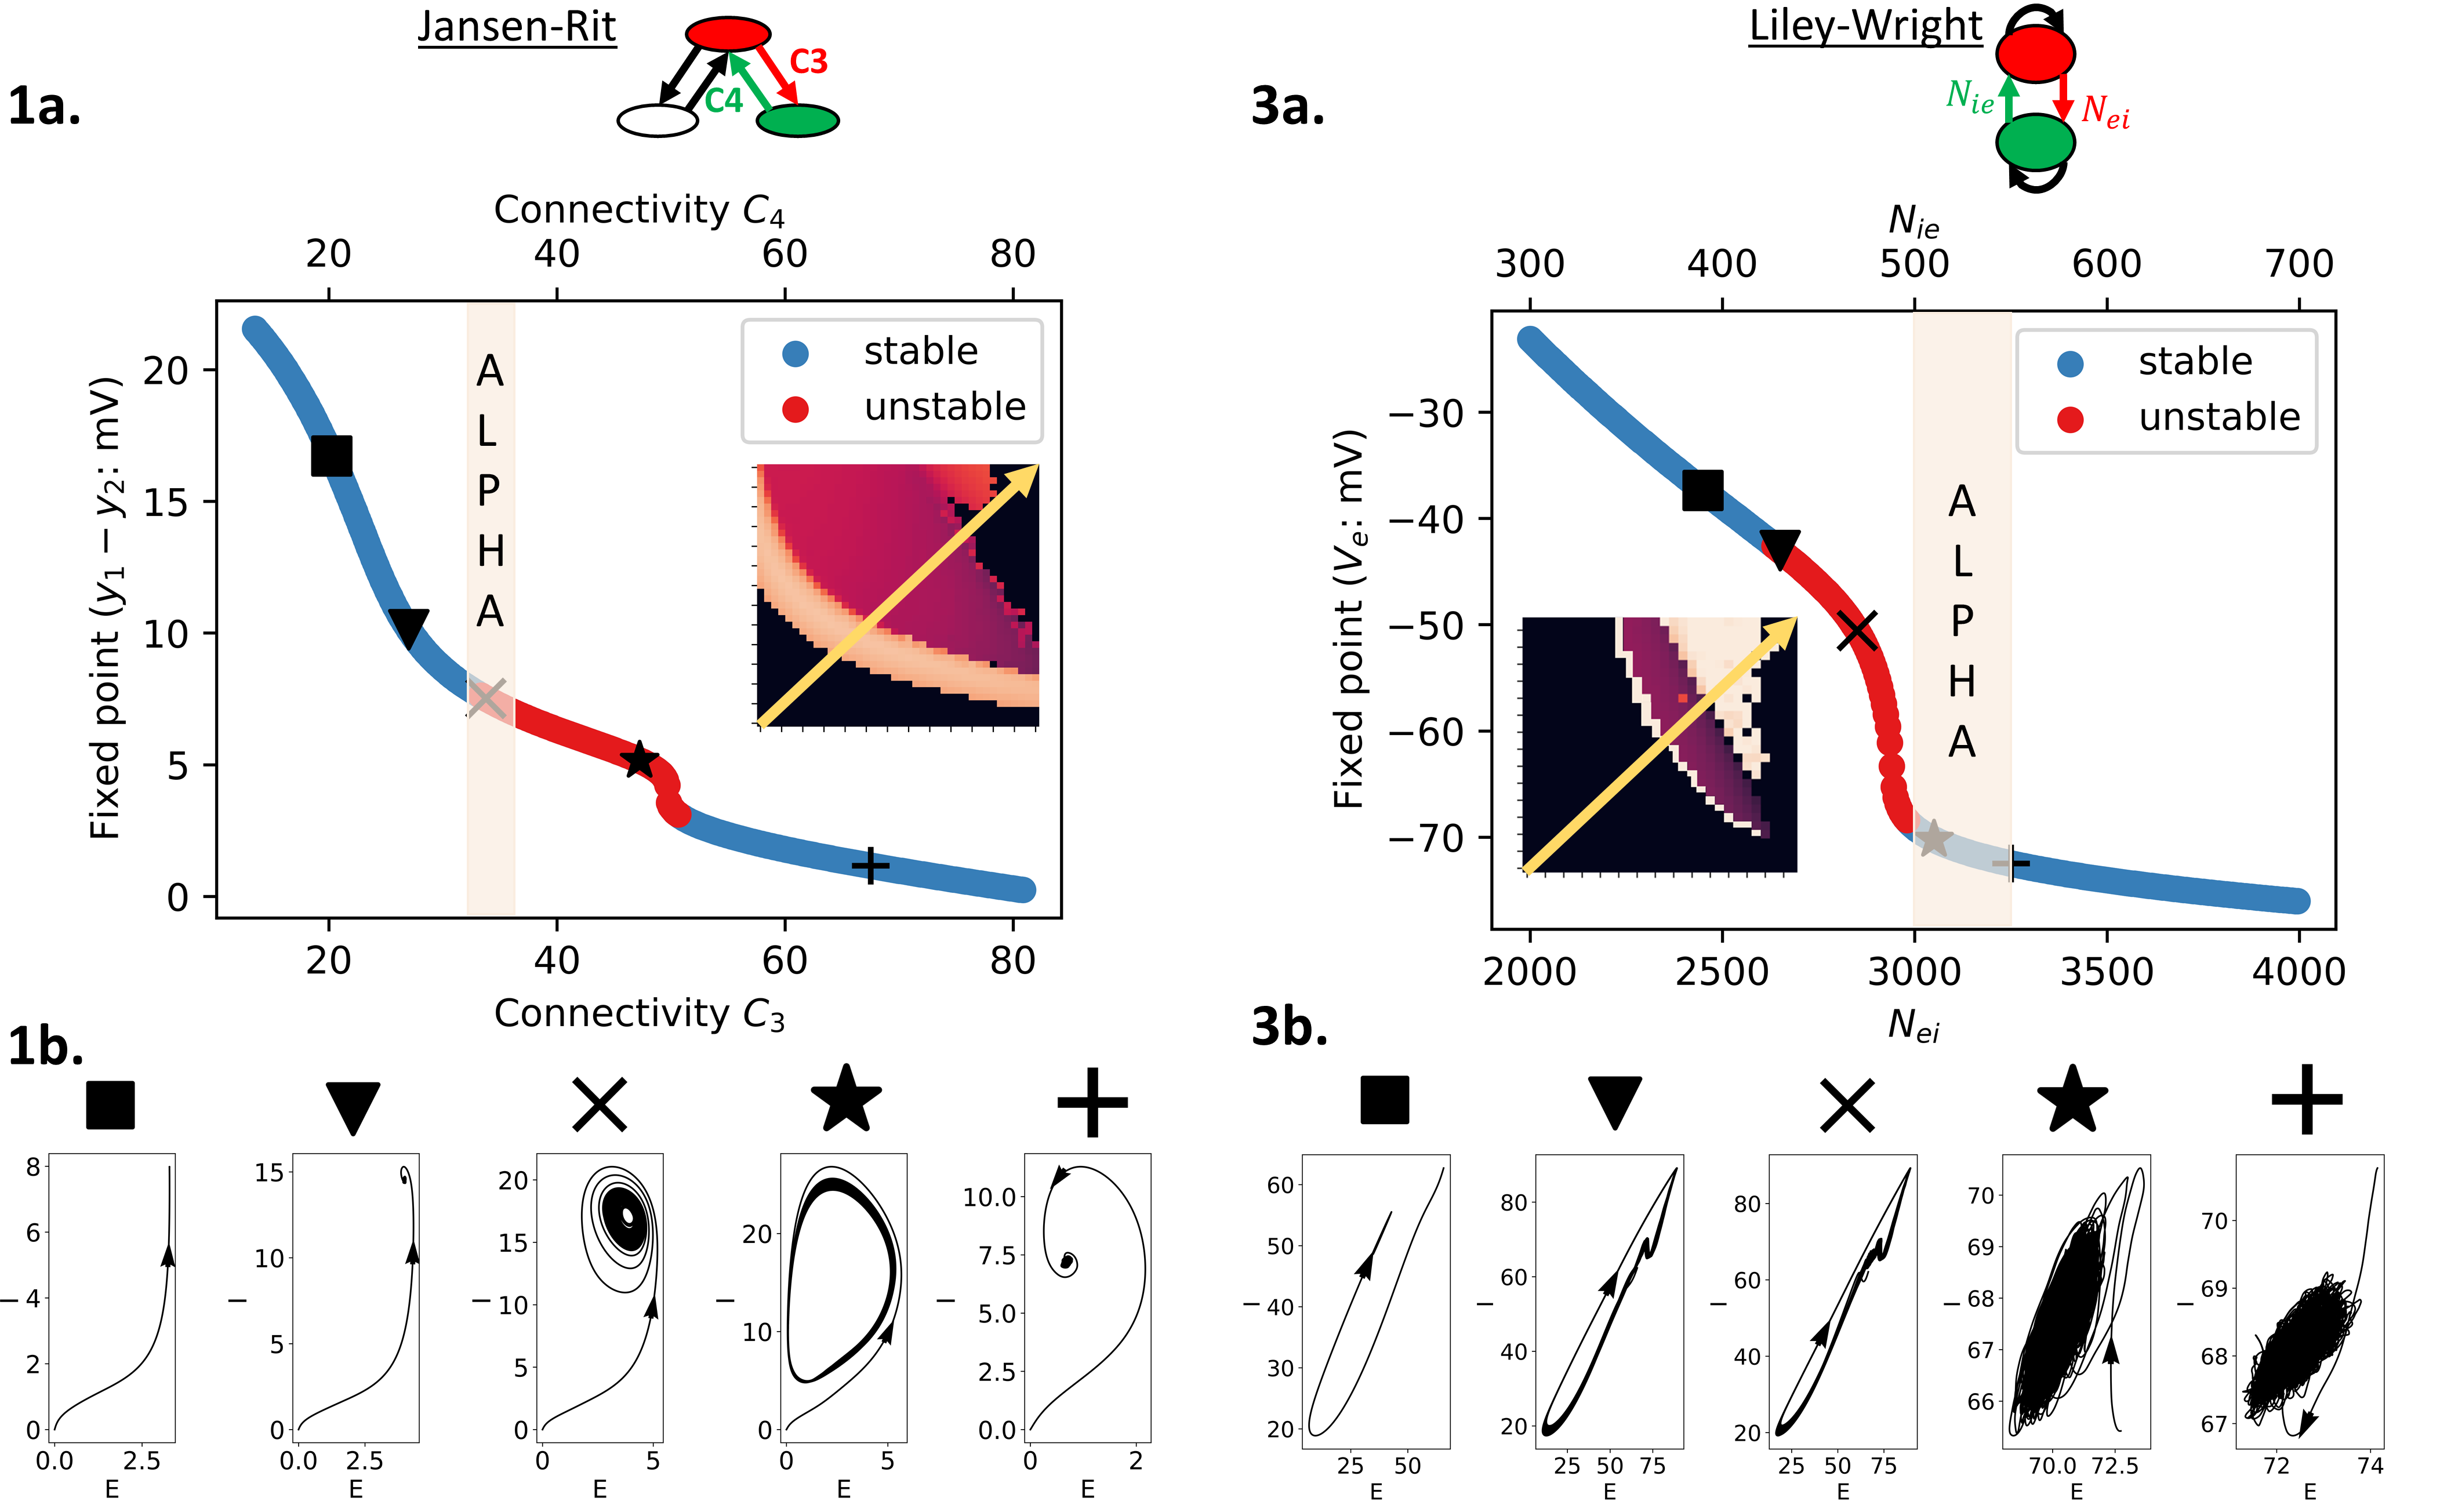
\includegraphics[scale=0.4]{Images/Stability_noise_2.png} %0.49
    %\centering
    %\hspace*{-0.3cm}
    %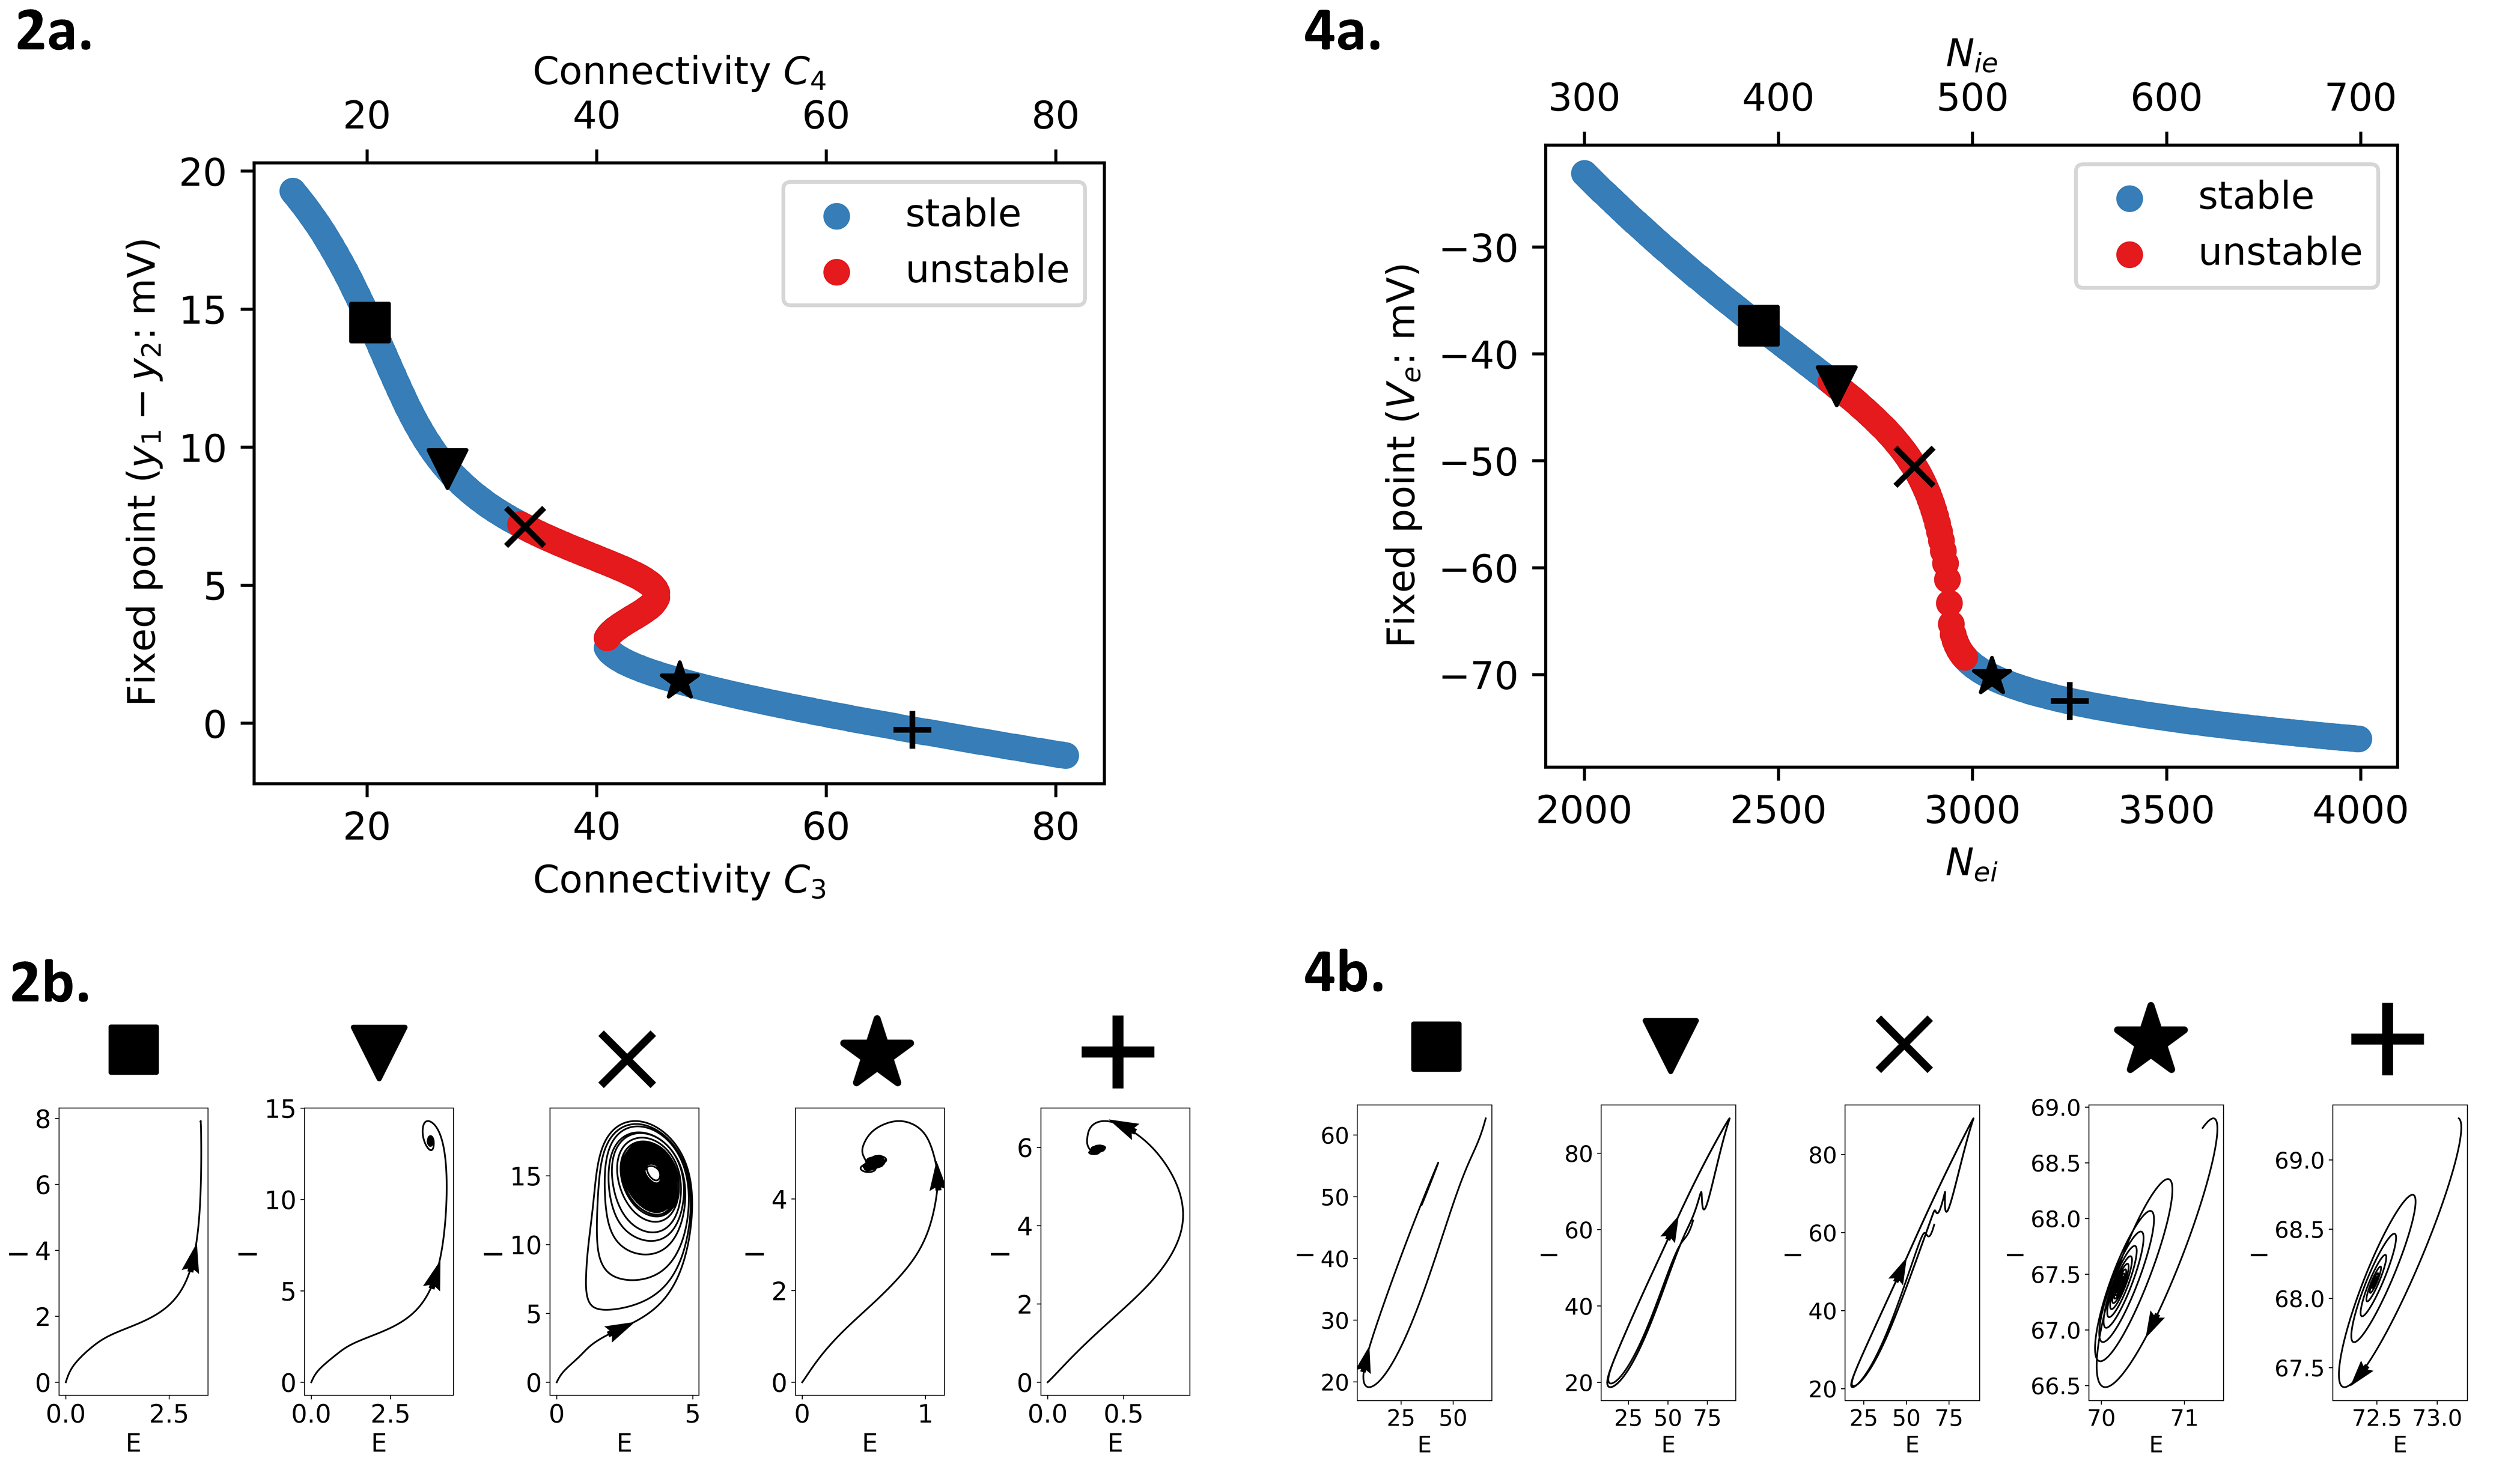
\includegraphics[scale=0.4]{Images/Stability_low_noise_2.png}%0.49
    \caption*{\textbf{Figure 11.  \textit{Fixed points and corresponding phase planes of JR and LW at specific connectivity values with high and low noise}} By performing stability analysis, the stability of the fixed points of JR and LW is determined for connectivity values intersecting across the parameter space (yellow arrow). For JR, A1 are the fixed points and A2 is the phase plane for specific values of connectivity. Similarly to JR, in B1 the fixed points of LW are presented with the corresponding phase plane in B2. Unstable fixed points are red, whereas stable fixed points are blue. The light orange area corresponds to the optimal connectivity parameter setting to generate alpha oscillations in each model.} \label{fig:Fixed_points}
\end{figure}
%TC:endignore
%These findings enhance our understanding of the relationship between E-I connectivity, alpha oscillations, and the specific mechanisms at play in the LW and JR models. They emphasize the importance of striking a balance in synaptic connectivity and shed light on the key role of corticothalamic interactions in generating and modulating alpha rhythms.
%TC:ignore
\vspace{-1.15cm}
\subsection{Comparative evaluation of models}
%TC:endignore
\vspace{-0.15cm}

\subsubsection{Topology, equations, and unified parameter table}

\vspace{-0.15cm}

Initially, we compared models within the alpha regime and explored different dynamical regimes through parameter space searches. However, explicit comparisons of model components, such as topology, equations, and parameter values have not been conducted. This section addresses these aspects to evaluate the validity and suitability of models as theories of alpha rhythm generation. 
\vspace{-0.1cm}


%\begin{figure}[H]
%\centering
   % 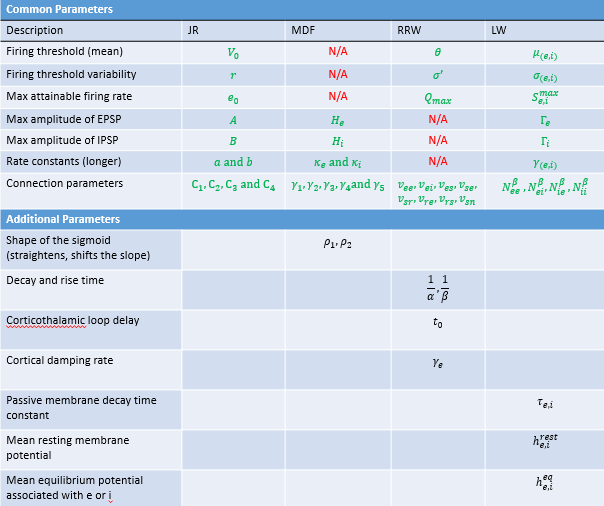
\includegraphics[width=0.95\linewidth]{Images/Unified_Param_Table.png}
   % \caption*{\textbf{Figure 25.  \textit{Table unifying parameters across models based on their biological interpretation.}} Common parameters are highlighted in green. JR,  }     
   % \label{fig:Param_Table}
%\end{figure}

%\rowcolors{2}{gray!20}{gray!70}
\begin{wraptable}{r}{11.5cm}
%\begin{table}[H]
    \centering
    \tiny
    %\scriptsize
    \begin{tabular}{ccccc}
        \rowcolor{black} 
        \multicolumn{5}{|c|}{\textcolor{white}{Common Parameters}} \\
        \hline
        \rowcolor{gray!70}
        Model & JR & MDF & LW & RRW \\
        \rowcolor{gray!20}
        Firing threshold (mean) & $V_{0}$ & -- & $\mu_{e,i}$ & $\Theta$   \\
        \rowcolor{gray!70}
        Firing threshold variability & $1/r$ & -- &  $\sigma_{e,i}$ & $\sigma'$\\
        \rowcolor{gray!20}
        Maximum firing rate & $2e_{0}$ & -- & $S_{e,i}^{max}$ & $Q_{max}$ \\
        \rowcolor{gray!70}
        Maximum EPSP amplitude & $A$ & $H_{e}$ & $\Gamma_{e}$ & -- \\
        \rowcolor{gray!20}
        Maximum IPSP amplitude & $B$ & $H_{i}$ &  $\Gamma_{i}$ & -- \\
        \rowcolor{gray!70}
        Rate constants & $a$ and $b$ & $\kappa_{e}$ and $\kappa_{i}$ &$\gamma_{e,i}$ & --  \\
        \rowcolor{gray!20}
         &  &  &  & $\nu_{ee}, \nu_{ei}, \nu_{es}, \nu_{se}$\\
        \rowcolor{gray!20}
        \multirow{-2}{*}{Connectivity} & \multirow{-2}{*}{$C_{1}, C_{2}, C_{3}, C_{4}$} & \multirow{-2}{*}{$\gamma_{1}, \gamma_{2}, \gamma_{3}, \gamma_{4}$} & \multirow{-2}{*}{$N_{ee}^{\beta}, N_{ei}^{\beta}, N_{ie}^{\beta}, N_{ii}^{\beta}$} & $\nu_{sr}, \nu_{rs}, \nu_{re}, \nu_{sn}$ \\ 
        \rowcolor{black} 
        \multicolumn{5}{|c|}{\textcolor{white}{Additional Parameters}} \\
        \rowcolor{gray!70}
        Sigmoid shape & & $\rho_{1}, \rho_{2}$ &  &  \\
        \rowcolor{gray!20}
        Decay and rise time & & & & $\frac{1}{\alpha},\frac{1}{\beta}$ \\
        \rowcolor{gray!70}
        Corticothalamic loop delay & & & & $t_{0}$ \\
        \rowcolor{gray!20}
        Cortical damping rate & & & & $\gamma_{e}$ \\
        \rowcolor{gray!70}
        Passive membrane decay & & & & \\
        \rowcolor{gray!70}
        time constant & & &\multirow{-2}{*}{$\gamma_{e,i}$} &\\
        \rowcolor{gray!20}
        Mean resting  & & & & \\
        \rowcolor{gray!20}
        membrane potential & & & \multirow{-2}{*}{$h_{e,i}^{rest}$}& \\
        \rowcolor{gray!70}
        Mean equilibrium potential & & & $h_{e,i}^{eq}$& \\
    \end{tabular}
        \caption*{\textbf{Table 2. \textit{Common parameters across models based on their biological interpretation.}} Certain parameters have a similar role and a biological interpretation associated with it that is comparable between the models. The additional parameters reflect the novelty and differences proposed by each models.
        \vspace{-0.5cm}}  
    \label{tab:global_eval}
%\end{table}
\end{wraptable}
NPMs typically include both excitatory and inhibitory neurons. For example, LW, with a single excitatory and inhibitory population, captures excitatory-inhibitory balance and includes synaptic reversal potentials and transmitter kinetics like fast AMPA and GABA. JR adds an excitatory population, resulting in three neural populations and reflecting Katznelson's approach to explore long-range excitatory connections \citep{katznelson1981normal, jansen1993neurophysiologically}. MDF introduces an inhibitory self-connection to account for high-frequency oscillations \citep{moran2007neural}, while RRW, with four neural populations, includes cortical and thalamic neurons and features complex connectivities. All models use second-order differential equations combined with a nonlinear operator for synaptic processes. JR does not separately simulate EPSPs and IPSPs for pyramidal cells, unlike MDF, which includes recurrent inhibitory connections and additional differential equations. MDF also features a richer sigmoid function definition with parameters $\rho_{1}$ and $\rho_{2}$ for voltage sensitivity and position, and adaptation currents through parameter $a$. LW is more complex due to an additional block converting postsynaptic potentials into soma membrane potential and includes fast neurotransmitter kinetics. RRW describes firing behavior using a damped wave equation for cortical excitatory populations, adding an additional $\phi_e$ term for average pulse density. Understanding the role and rationale of different parameters is essential for making models biophysically meaningful. S.9 includes parameter tables and their biological meanings. While all the models share common components, MDF allows easier modulation of the sigmoid function shape, and RRW introduces corticothalamic interaction parameters. 
LW incorporates synaptic reversal potentials, distinguishing its dynamic transformation of postsynaptic to soma membrane potentials.

%\vspace{-1.5cm}


%TC:ignore
\subsubsection{Biological basis and rationale of parameter values}
%TC:endignore
The systems under consideration have parameters with corresponding biological interpretations; however, the nominal values assigned to these parameters vary considerably across the models. The variation in parameter values across the models can be attributed to several factors, including differences in the experimental data used to inform the models, distinct mathematical formulations, and specific assumptions. Each model is designed to capture different aspects of neural activity and may prioritize certain features or phenomena over others. In the following section, we first examine the rationale behind the expression and parameters of the firing rate function, then the impulse response, and finally the connectivity values. 

%Even though MDF is an extension of JR, in \citet{moran2007neural}, the authors deliberately selected `standard' parameters that prioritize an engaged synchronized EEG with significant power in the higher beta frequency range, aiming to showcase the impact of nonlinearities in their computational framework. The standard MDF parameters are thus adjusted here to place the central frequency in the alpha band by using comparable values \citet{david2003neural}. %or is it David and Friston 2005 
%herefore, parameter values of JR and MDF impulse response and firing rate function are of the same order, and can be traced back to three key authors: \citet{freeman1974model, freeman1975mass, freeman1987simulation, freeman1979nonlinear}, \citet{lopes1974model, da1976models}, and \citet{van1982model}.
%As mentioned in section 2.2.1, Freeman's work is a source for numerous parameter values in NPMs, which were empirically assessed based on detailed physiological studies of the olfactory bulb. 

\paragraph{\textit{Firing rate}} ~\\
Fig. 12 shows the firing rate curves of the four models. It can be seen here that there is some variability in maximum neural firing rate parameters used, as well as the point of inflection of the curves. As mentioned in the previous section, MDF implements a different expression of the sigmoid that does not include parameters equivalent to a maximum firing rate, mean firing threshold, or standard deviation of the threshold distribution in the neural population, but instead has two parameters defining shape and position. The maximum amplitude with the current setting reaches 0.9, but can be tuned by modifying the parameters $\rho_2$. Even though the other three models have parameters with a similar biological interpretation, the values are considerably different. First, the maximal firing rate is equal to $500s^{-1}$, $340s^{-1}$ and $5s^{-1}$ for LW, RRW, and JR respectively. The difference in the order of magnitude between JR and the other two models (LW and RRW) can in part be explained by the fact that the value chosen by Jansen and Rit in their original paper is taken from \citet{freeman1987simulation}, and is actually a dimensionless normalized parameter. This quantity is expressed without units (for details on the calculation of the maximal wave amplitude $Q_{m}$ see \citealp{freeman1979nonlinear}), whereas both RRW and LW rely on experimentally derived average values. However, in the case of RRW, the assumed $Q_{max}$ value was made without a clear citation, indicating that this is an assumption, and is given in units of the maximum possible value \citep{robinson1997propagation, rennie1999effects}. The standard values from Freeman for converting membrane potential to firing rates are applied in the JR firing rate function, but the expression itself stems from \citet{da1976models}, and the current JR model uses a simplified version of that function. In the case of RRW, the firing rate function initially corresponded to the error function introduced by \citet{wright1995simulation}. Since 1999, the nonlinear function in RRW has been a modified version of that initial error function and closely approximates it \citep{rennie1999effects}. The differing source of the firing rate conversion equation between the two models explains the slight differences observed in their mathematical expressions. 

%Whereas, RRW and LW values are averages found experimentally. Although, for RRW, it is mentioned that the value of $Q_{max}$ is an assumption that was made (source) and no source seems to be cited.
The spiking threshold parameter (voltage at point of inflection in the sigmoid curve) in LW has a negative potential, due to the fact that the model includes synaptic reversal potentials. JR and RRW, in contrast, have a positive point of inflection for this parameter ($6mV$ and $12.92mV$ respectively). The values for the standard deviation of the threshold distribution in the neural population, which affects the steepness of the firing ate slope, are $(1/0.56)mV$ ($\approx 1.79mV$), $5.5mV$, and $5.9mV$ for JR, LW, and RRW respectively.  
%didnt talk about the variability
%TC:ignore


%\vspace{-0.5cm}

\begin{figure}[H]
    \hspace{-0.5cm}
    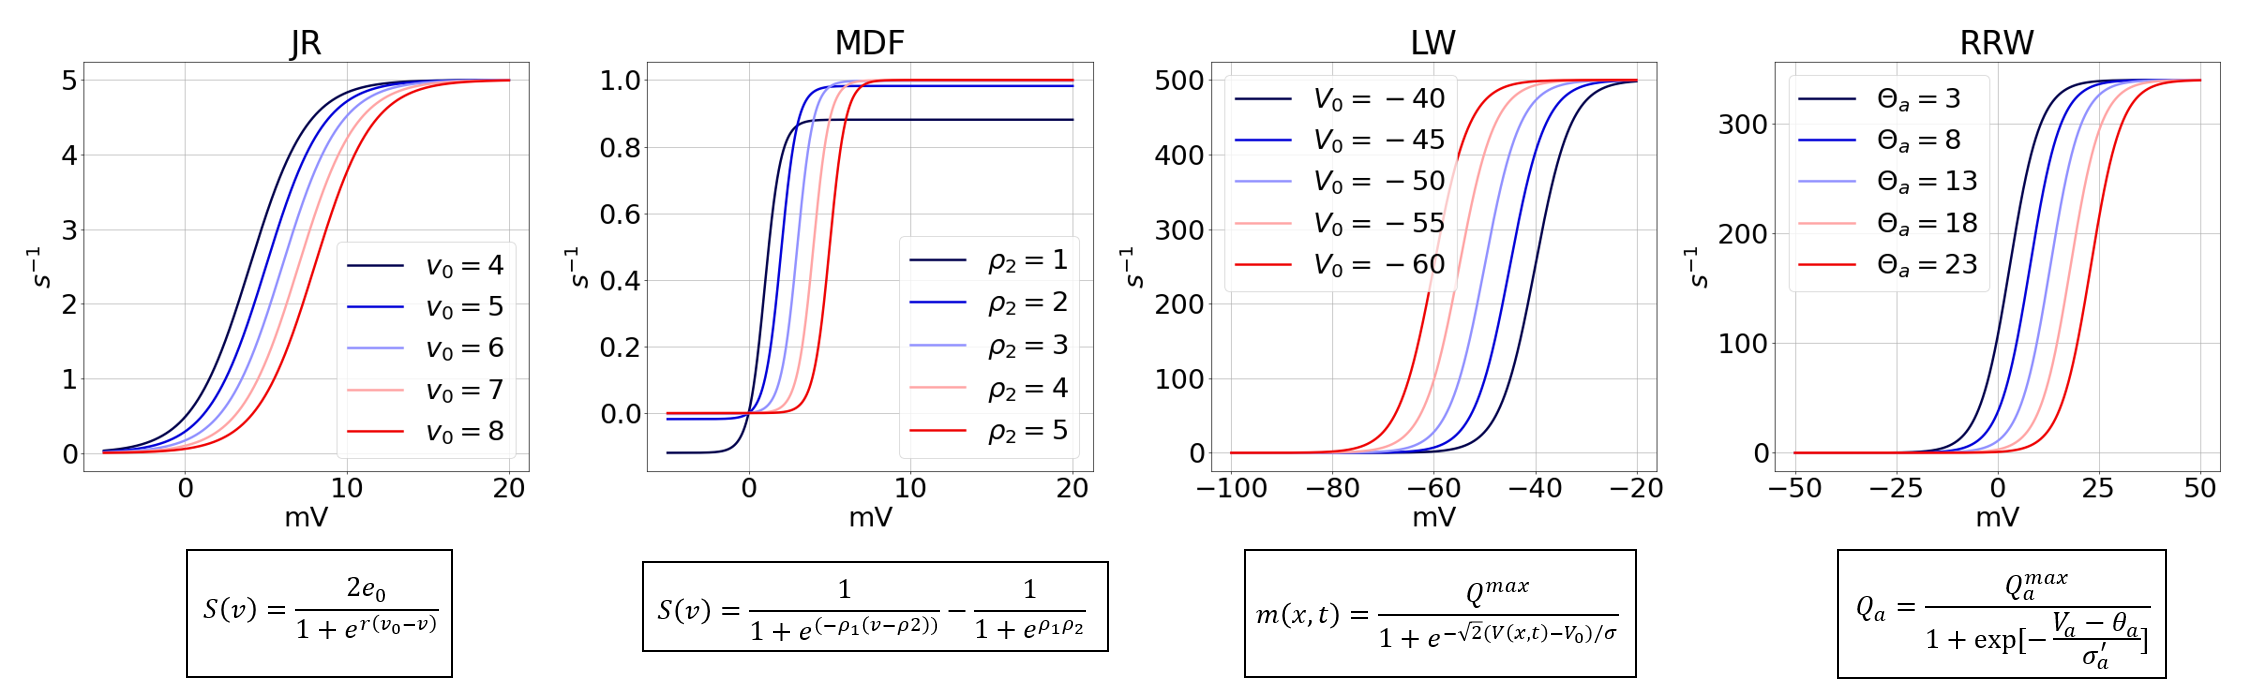
\includegraphics[scale=0.3]{Images/Sigmoid_3_1.png}
    %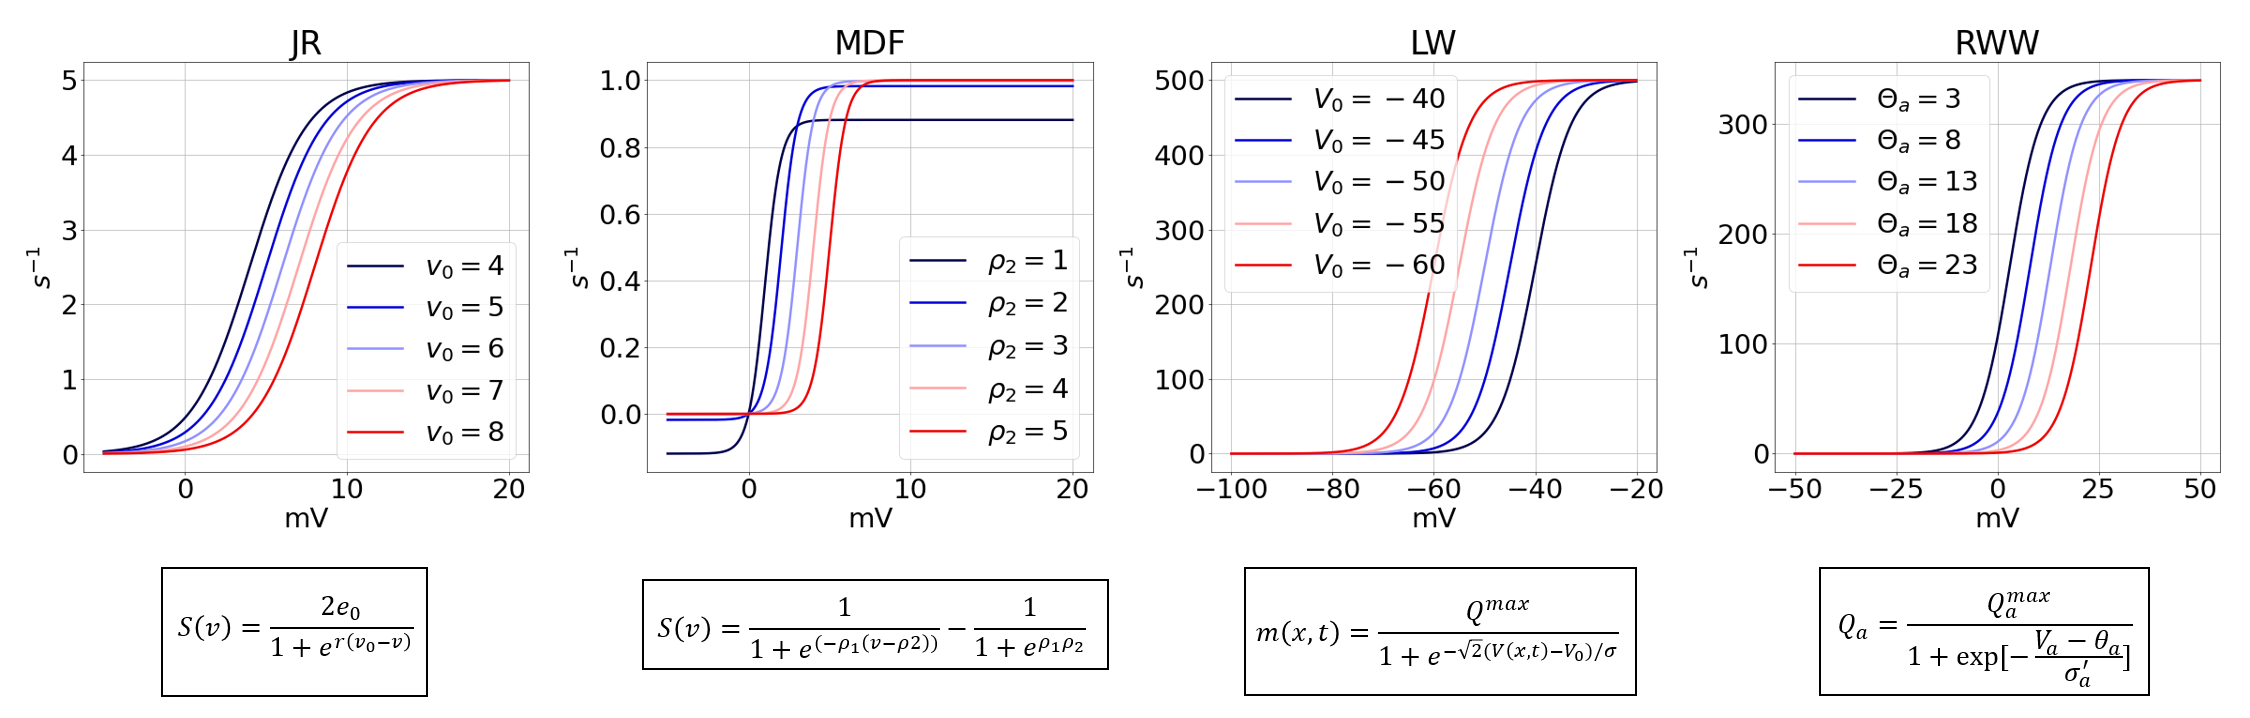
\includegraphics[scale=0.5]{Images/Sigmoid_2.png}
    \caption*{\textbf{Figure 12.  \textit{Sigmoid curve of each model with firing rate against voltage with different firing threshold.}} The sigmoids differ in terms of the maximum value and the voltage at which the inflection point occurs which is modulated by the firing threshold.}     
    \label{fig:JR_Sigmoid}
\end{figure}
%TC:endignore

\vspace{-1cm}

\paragraph{\textit{Impulse response}}~\\ 
With respect to the impulse response, the parameter values in JR can be traced back to \citet{van1982model}. The impulse response used in JR corresponds to a simplified version of expression given in Lopes Da Silva \citet{lopes1974model, da1976models}. These authors determined the parameters $A$, $B$, $a$ and $b$ by respecting certain basic properties of real postsynaptic potentials, and ensuring the system produces alpha frequency oscillations \citep{grimbert2006analysis}. This choice of JR to use the alpha function (unrelated to alpha rhythms) as an impulse response was originally proposed by \citet{rall1967distinguishing}. 
MDF has an identical impulse response function, but some of the standard parameter values differ because in \citet{moran2007neural}, the authors deliberately selected `standard' parameters that prioritize an EEG with significant power in the higher beta frequency range, aiming to showcase the impact of nonlinearities in their computational framework. The standard MDF parameters are thus adjusted in the present study to place the central frequency in the alpha band by using comparable values to \citet{david2003neural}. %or is it David and Friston 2005 
With our adjustments to obtain alpha oscillations, the values of the impulse response in MDF vary slightly from those in \cite{moran2007neural}, such as the rate constants ($250s^{-1}$ instead of $100s^{-1}$ for $\kappa_e$; $62.5s^{-1}$ instead of $50s^{-1}$), but are still in the same order of magnitude. These differences are explained by the fact that the additional self-inhibitory connection changes the behavior of the system for similar parameter values. Thus, to simulate an equivalent alpha these need to be modified.
%One notable difference that is in \cite{moran2007neural} is the maximum amplitude of IPSP in MDF which is equal to 22mV instead of which to the one proposed earlier by Lopes Da Silva 1974 instead of van Rotterdam (32mV instead of 22mV). --> with our modification in the end IPSP is 22 but EPSP is 10
There is some variability across the models in the values used for EPSP and IPSP amplitudes. This has been justified physiologically by the fact that certain neuropeptides can modulate the amplitude of PSPs, meaning that some degree of freedom in choice of these values is needed \citep{jansen1995electroencephalogram}.
For the dendritic response, the original RRW model paper \citep{robinson1997propagation} mentions using `physiologically reasonable parameters' for the decay and rise rate ($\alpha$ and $\beta$), and cites sources such as \citet{freeman1991induced}, \citet{lopes1974model}, and \citet{van1982model}, with no further details provided. It is surprising that the peak of the dendritic response is around 60mV, which is considerably higher than the other models. LW, on the other hand, has a lower potential peak amplitude, which may be due the fact that other models represent the voltage at the soma, whereas LW expresses it at the site of synaptic activation \citep{liley2001spatially}. One of the status intentions of LW relative to its predecessors was to be more physiologically realistic, and thus allow greater biological validity and interpretability of its parameters \citep{liley2001spatially}; however it is notable that very little detail is given about the sources for chosen parameter values. %LW assumes that the parameters are time invariant. %(question is this the case for every model?). 
Overall, an anatomical assumption made is that the amplitude of the inhibitory impulse response is larger than the excitatory impulse response, due to the fact that the former have axon terminals closer to the cell body, thereby leading to larger perturbation upon synaptic transmission \citep{kandel2000principles,cook2021neural}. LW makes the (reasonable) assumption that excitatory impulses occur on a faster timescale than inhibitory impulses, which is shared with JR and MDF, but notably not with RRW. In Fig. 13, the shape of each model's excitatory and inhibitory impulse responses are shown, with their nominal varying rate constant values. As the rate constant increases, the curve widens and the decay time increases. In the case of RRW but not JR, MDF, or LW, variation of the decay time also leads to changes both slope and the magnitude of the impulse response curve.
%TC:ignore

\vspace{-0.1cm}

\newline

\begin{figure}[H]
    \hspace{-0.5cm}
    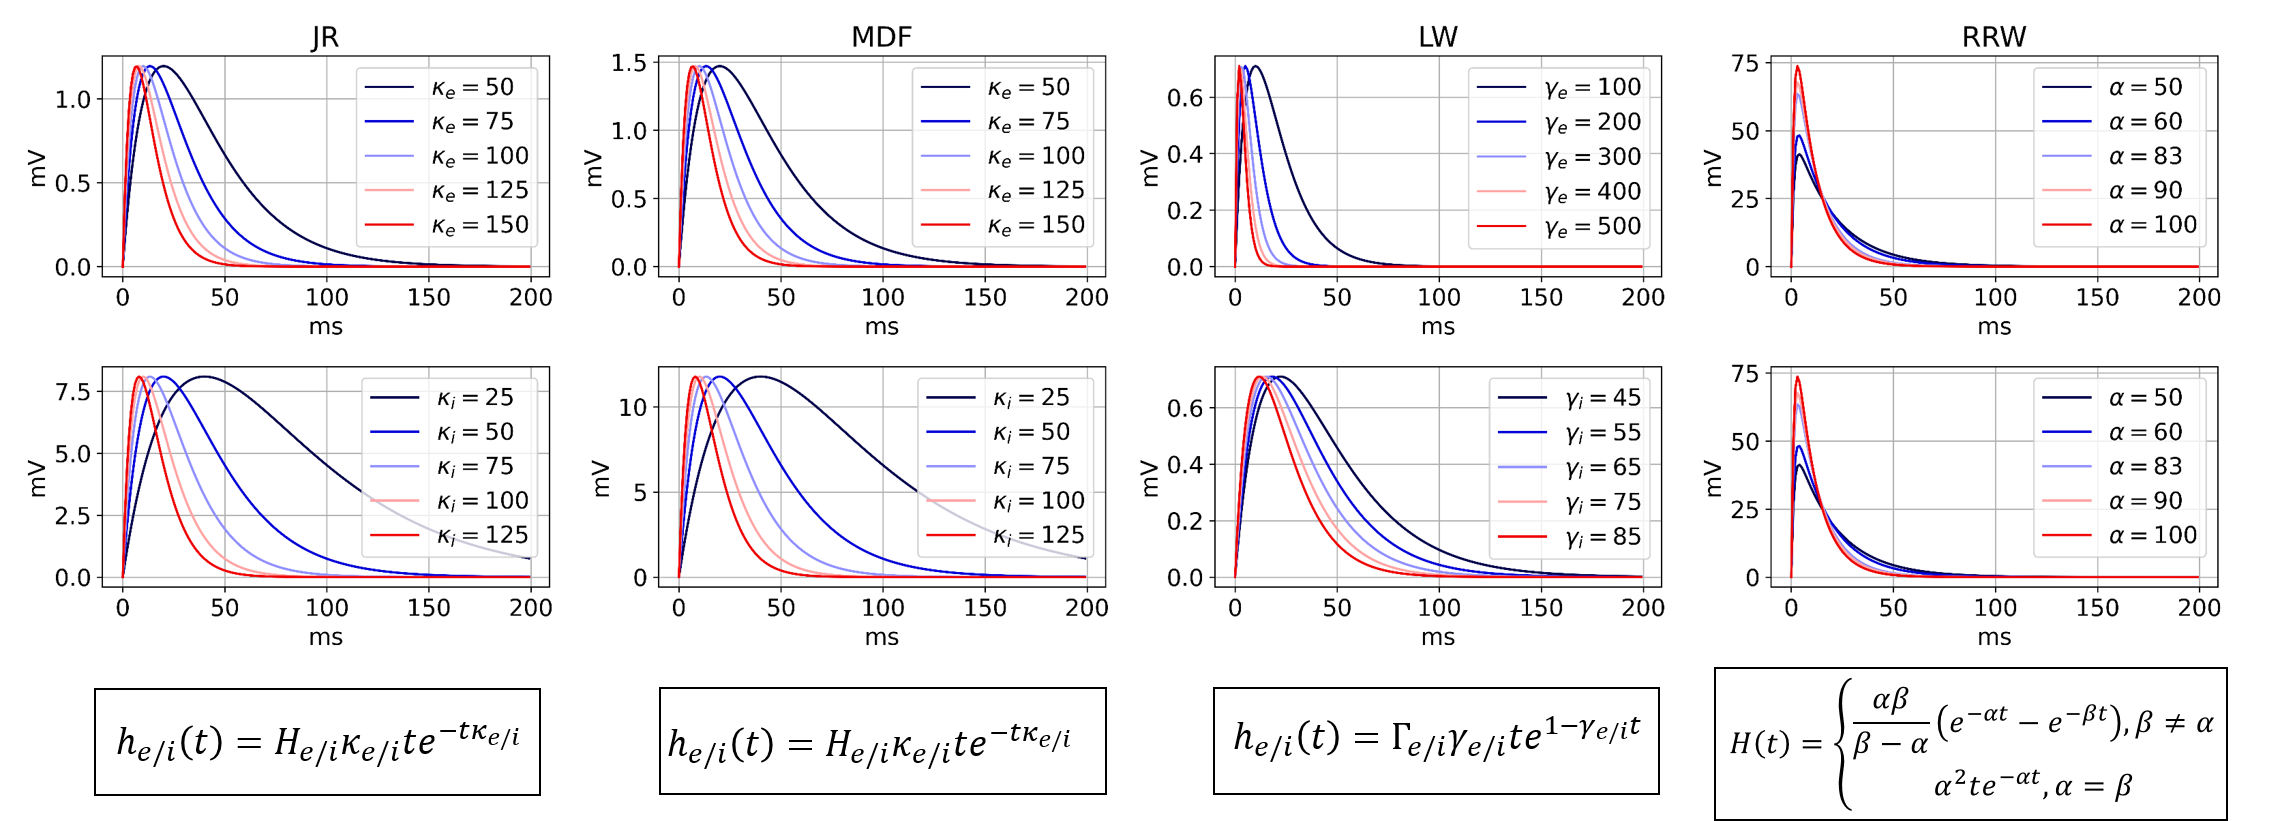
\includegraphics[scale=0.3]{Images/Impulse_response_3_1.png}
    %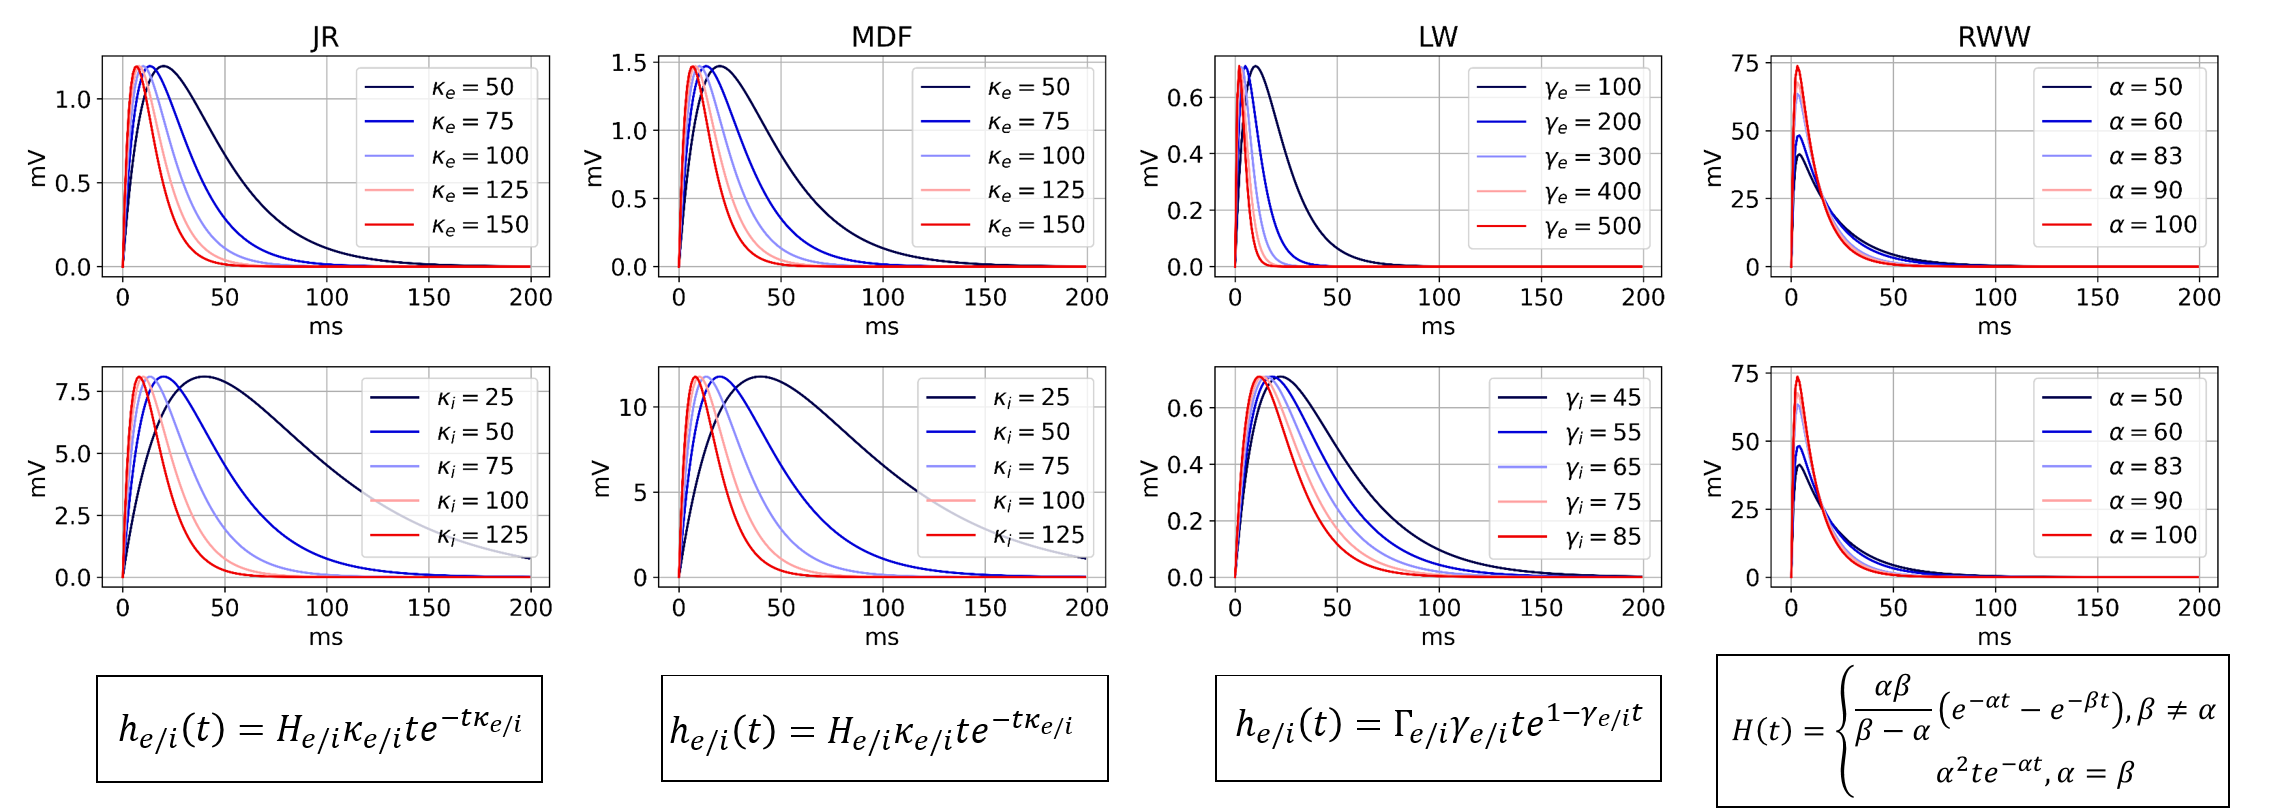
\includegraphics[scale=0.48]{Images/Impulse_response_2.png}
    \caption*{\textbf{Figure 13.  \textit{Impulse response of excitatory and inhibitory population with varying rate constant}} Top: EPSP; Bottom: IPSP; except for RRW which uses the same dendritic response curve for EPSP and IPSP. The general shape of EPSP and IPSP between the models is consistent and mainly differ in terms of amplitude. Rate constant is varied for the first three models and for RRW, the different curves correspond to varying decay times. }     
    \label{fig:JR_impulse}
\end{figure}
%TC:endignore
\vspace{-1cm}
\paragraph{\textit{Connectivity}}~\\
Connectivity parameters across the four models differ in their units and physiological interpretation, making direct comparisons of specific values challenging. In JR and MDF, the connectivity parameter values are dimensionless, and proportional to the average number of synapses between populations \citep{jansen1995electroencephalogram}. Based on several neuroanatomical studies \citep{braitenberg2013cortex, larkman1991dendritic, liu1991distribution, elhanany1990intrinsic} that estimated these quantities by counting synapses. With these studies, Jansen and Rit condensed the four connections into fractions of a single parameter C \citep{grimbert2006bifurcation}. Since Jansen and Rit estimated that the global parameter C would most likely change primarily due to its role in capturing synaptic phenomena like neurotransmitter depletion, this reduction has been useful in determining the overall effect of variations in connectivity while keeping their proportions to each other identical. LW has parameters representing the total number of connections between the two populations, which take higher values for excitatory neurons as 80\% of cortical neurons are excitatory \citep{cook2021neural}. Furthermore, anatomical estimates for each connection were derived using an equation that considers the diameter of the mean dendrite and intracortical axon, the mean total length of all dendritic and intracortical axonal arborizations, the mean length of the pyramidal cell's basal dendritic arborizations, and the neuronal density (as described in \citealp{liley2001spatially} and outlined in \citealp{liley1994intracortical}). RRW has connectivity variables denoted as $\nu_{ab}$, which correspond to the mean number of synapses (anatomical or structural in nature) multiplied by the strength of the response to a unit signal expressed in units as $mVs$ \citep{rennie1999effects, robinson1997propagation, rall1967distinguishing}. 
 
% Need transition

In summary, we have sought in this section to compile information from the literature on the origin of the mathematical expressions, parameter values, and  biological motivations of our four models. Notable observations include: i) even though the formulation of the firing rate curves is similar between JR, LW and RRW, their mathematical origin differs, with \citet{da1976models} as a reference for JR, and the error function introduced by \citet{wright1995simulation} for LW and RRW; ii) there is some variability across models in the parameters and equations for the impulse response; iii) connectivity parameters can represent a proportion of the average number of synapses (JR and MDF), a total number of synapses (LW), or synaptic strengths (RRW); iv) Although the specific parameter values may vary for the firing rate and the impulse response, modifying them uniformly yields a consistent effect across the two curves (Figs. 12 and 13); and v) similarly, as shown in Fig. 10, correspondences can be made in the effects of altering connectivities.

%Additionally, the models have different regions of stability and are able to produce other types of oscillations. Defining the parameter space of those different regions for each model allows for comparison in the behavior of the system/model.
%Add effect of input and choices.


% mini summary

% - identified, described, reviewed, analyzed alternative alpha models and theories and subcomponents etc

% new things:

% - alpha blocking: robinson, used params from prev papers; liley - same; JR - new result = do what liley did
% - can we do this with analytic models in that fig also?

% - rate constants fig (jr done before but comparison w liley and moran not)
% - 

% - E vs I param space comparing over models; diagonal sweet spot; angle of diagonal = asymmetry between E and I variation; non-alpha behaviour off the diagonal (fig 11)

% fig  12 - bif analysis - all new (?)
% confirmation that alpha 'mechanism' (mathematically at least = bifurcation type) is different between JR and LW

% param comparisons (*notable points?)

% sigmoids and impulse responses - key points?

%TC:ignore
\section{Discussion}

%We compared the four prominent intracortical and corticothalamic models above to investigate the dynamics and mechanisms of alpha rhythms through local circuits. 

\subsection{Summary of main findings}
%TC:endignore
In this paper, we systematically investigated the major mathematically-expressed physiological theories of EEG alpha rhythmogenesis, focusing on four primary models (JR, MDF, LW, RRW) that cover the two main alpha theory types - intracortical and corticothalamic \citep{nunez2006electric}. Our aim was to clarify the relationships between these models to prepare for future experimental and theoretical work. We examined the mathematical expression of each model, highlighting common elements and differences, and explored their parameter space to identify conditions producing alpha rhythms, focusing on rate constant and E-I connectivity strength parameters. We reported confirmatory simulation results and several novel findings. Despite differences in elements such as nominal cell types, microcircuit topologies, and connectivity assumptions, all models can reproduce the characteristic features of resting state alpha observed in empirical EEG data, with RRW better capturing the 1/f scaling and JR and LW showing more attenuated alpha blocking (Fig. 8). We also examined the effect of changing the rate constant on the dominant frequency of oscillation, finding that MDF demonstrates a larger range of oscillatory behavior. Our comparative simulations highlighted differing positions of the hypersignal regime between JR, MDF, and LW, and demonstrated the significant impact of E-I connection strengths on model dynamics. In JR, the total connectivity strength of the inhibitory loop determines the oscillatory regime. In RRW, we observed that the intrathalamic E-I loop also plays a crucial role in modulating the general dynamics of the alpha oscillation. Decreases in inhibition lead to a dominant beta-frequency peak, and a slight shift in the alpha central frequency. However, the primary effect of the RRW intrathalamic loop (within the parameter regimes studied) was seen to be modulation of alpha peak amplitude. 

Finally, we observed that changes in the number and strength of GABA interneuron synapses in LW tend to have a more prominent effect on the dynamics compared to the corresponding GABA-related parameters of the other models.
Exploring the stability of the JR and LW models revealed different mechanisms for generating standard alpha oscillation: a self-sustained limit-cycle for JR and noise-driven fluctuations for LW. 
Our comparative evaluation highlighted topological and mathematical differences and clarified the rationales behind parameter values. Despite variations, the impact on the shape of both the sigmoid and impulse response is consistent (Figs. 12-13). Our investigation shows similar capacities to generate spectral EEG features, leaving it unclear which alpha theory type is best supported. The selection of a model depends on the study's goal, its capacity to represent neural activity features, and relevant biological details. While mesoscopic scale empirical data may be insufficient to favour one alpha theory over another, our study clarifies the role of the E-I loop in each model and the implications of synaptic gains on dynamics, which we hope will prove useful in studies of altered dynamics associated with neural pathologies and disorders \citep{eichler2008ei, li2022excitation}.


%TC:ignore
\subsection{Model limitations and critique}
%TC:endignore
NPMs offer a valuable framework for studying brain dynamics at the mesoscopic scale using data from EEG, MEG, LFPs, ECoG, fMRI, PET, fNIRS, and wide-field calcium imaging. However, their simplicity sacrifices important neurobiological details, posing challenges for parameterization and validation, particularly in the lack of correspondence between model variables and well-defined observable quantities and neural structures \citep{cook2021neural}. Experimental validation of NPMs of this kind has to date mostly relied on human EEG data, capturing cortical excitatory neurons, leaving cortical inhibitory and thalamic populations unmeasured. Complementary data from LFPs and advanced recording technologies, such as combined electrophysiological and optical imaging in rodents, can address some of these limitations, albeit with substantial species differences. NPMs bridge microscopic and macroscopic brain states but involve assumptions and abstractions that may disconnect understanding across spatial scales \citep{goldman2019bridging, huang2021novel, cook2021neural}. NMMs assume uncorrelated neuron states within ensembles \citep{breakspear2017dynamic}, neglecting within-population synchrony, which might impact observed EEG responses \citep{glomb2021computational}. The sigmoidal function used to transform membrane potential into firing rates is a phenomenological approximation \citep{huang2021novel, byrne2020next}, and individual neuron firing thresholds are thus not considered in these models.

Despite these caveats, NPMs do effectively represent brain dynamics at the meso/macro scale observed in scalp EEG, offering simplicity and computational efficiency. They enable numerical simulations, parameter estimation, and analytical correspondences for insights into physiological mechanisms \citep{david2006mechanisms, abeysuriya2014prediction, momi2023tms}. In addition to limitations inherent to all NPMs, each of the four models also has its own advantages and limitations. JR has a constrained oscillatory range and requires an external drive for stable alpha oscillations, which could be considered to be inconsistent with the empirical observations that intrinsic alpha power is strongest during eye-closed states \citep{kiani2021realistic}. MDF includes self-inhibitory connections and spike-rate adaptation terms for higher frequency ranges, but uses parameters with limited biological relevance \citep{moran2007neural}. LW incorporates conductance-based elements like synaptic reversal potentials, enhancing neurobiological fidelity but increasing numerical instability \citep{liley2001spatially}. RRW approximates EPSPs and IPSPs with the same impulse response, which has been debated, though it can reproduce empirical features like the 1/f curve and different oscillatory frequencies across brain states and neuropathologies \citep{roberts2008modeling, zhao2015generalized, muller2017unified}.

%\begin{figure}[H]
 %   \centering
  %  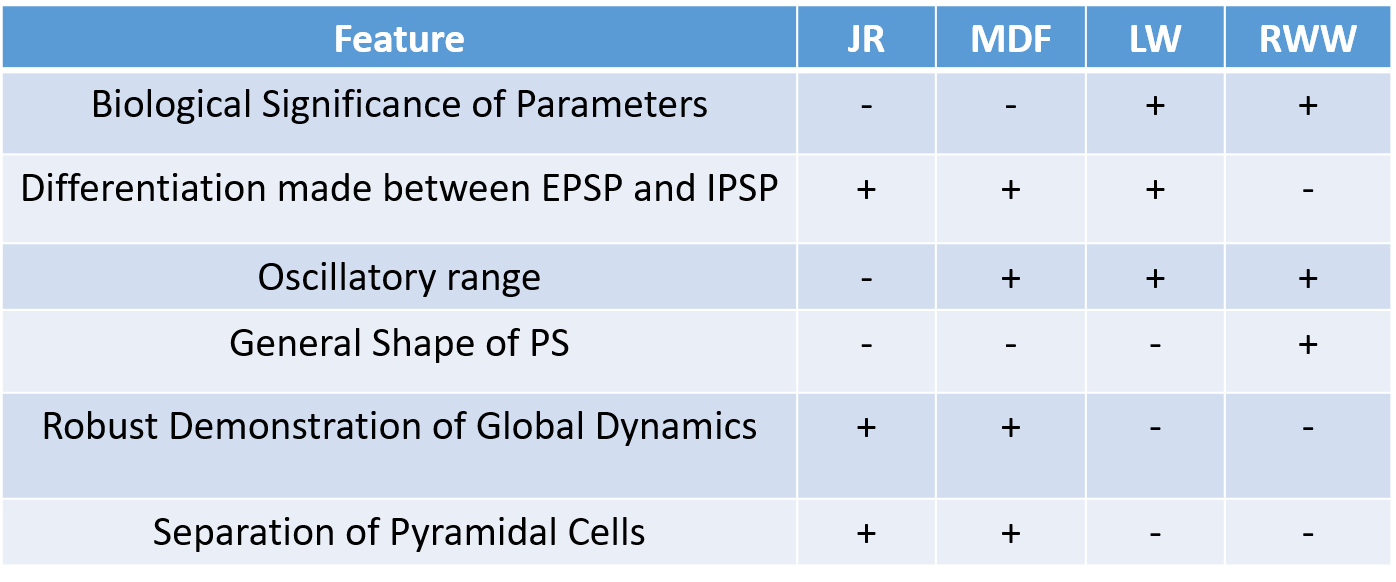
\includegraphics[scale=0.5]{Images/Table_global_eval.png}
   % \caption*{\textbf{Table.  \textit{Global evaluation of the models}} More details need to be given}   
   % \label{fig:Global_eval}
%\end{figure}
%\newpage 

\begin{wraptable}{r}{10cm}
%\begin{table}[]
    \scriptsize
    \rowcolors{2}{gray!20}{gray!70!}
    \centering
    \begin{tabular}{ccccc}
        \rowcolor{black} 
        \textcolor{white}{Feature} & \textcolor{white}{JR} & \textcolor{white}{MDF} & \textcolor{white}{LW} & \textcolor{white}{RRW} \\
        \hline
        Biological significance of Parameters & - & - & + & + \\
        Differentiation between EPSP and IPSP & + & + & + & - \\
        Oscillatory range & - & + & + & + \\
        General shape of PS & - & - & - & + \\
        Robust Demonstration of Global Dynamics & + & + & - & - \\
        Separation of Pyramidal Cells & + & + & - & -
    \end{tabular}
    \caption*{\textbf{Table 3. \textit{Global evaluation of the models.}} Different features of the models are assessed, highlighting strengths and limitations. In terms of robustness and tractability, the JR and MDF models prove more suitable. LW incorporates more physiological elements, and RRW shows a stronger capability in reproducing empirical features of alpha activity.} 
    \label{tab:global_eval}
    \vspace{-0.5cm}
%\end{table}
\end{wraptable}

A comparative analysis of these models (summarized in Table 3) reveals that the JR model shows robust global dynamics but has limitations in biological parameter significance and oscillatory range. The MDF model achieves higher frequency simulations but shares similar limitations. The LW and RRW models offer biologically associated parameters and a broad range of oscillatory frequencies, but robust global dynamics are challenging to demonstrate. The RRW model is promising for reproducing empirical features like the 1/f curve.


\subsection{Conclusion and future work}

% left this here as a maybe...
% is also still in the text block at the start of this chapter
In conclusion, our comparative analysis of the JR, MDF, LW, and RRW models elucidates their mathematical formulations and parameters, providing a range of biological insights. Our novel simulations showed differing precision in replicating EEG alpha characteristics, highlighting the impact of rate constants and connectivity parameters on their dynamical behavior.

Future studies of alpha rhythmogenesis in human EEG should investigate intracortical and corticothalamic models at the whole-brain scale. Mesoscale data from single neural populations alone may be insufficient to distinguish between these theories. A key objective should be to determine the role of the thalamus in generating resting state alpha oscillations, and more generally to adjudicate between the cortical and corticothalamic alpha theories. We hypothesize that topographic variation in oscillatory brain activity, as well as network-level connectivity and dynamics, will provide important additional information for this question. Whole-brain studies must consider each node's role in the larger network, as the dynamics of neural populations may change when interconnected via the connectome. Finally, improving validation methods against empirical data, for example by extending the number and type of EEG features used for model comparison and fitting, would allow for better differentiation between models and determination of which ones offer are more accurate representation of observed brain dynamics.



%\subsection{Concluding Remarks and Future Work}

%A central purpose of the paper was to compare existing popular intracortical and corticothalamic NPM that we deemed encompassing the different formulations and advanced research on the understanding of alpha rhythmogenesis. 
%The scope of our study is biologically inspired phenomenological models with a focus on rate constant and E-I connectivity parameters for a meaningful evaluation. 

%Validation of NPM against empirical data is a challenging task as of today it is mostly based on the visualization of EEG data representing the macroscale. Variables used at the mesoscopic scale do not have thorough empirical bases to compare against. Therefore, distinction between the models presented on an assessment against EEG data and relies on parameter space searches to identify general trends. Throughout this work, since similar behavior was identified namely in their E-I interactions, it is difficult to affirm confidently which one is better represent alpha oscillations and thus which theory is more plausible. However, each model have their respective advantages and limitations which will define their use cases. Choosing a model over another will depend on their capacity to represent certain features or the inclusion of more biological details. 
%However, at this scale, we were able to identify the role of the E-I loop in each model and how the gain will influence the dynamics represented as well as various alpha mechanisms. Biologically, shows how imbalance in E-I can lead to altered dynamics (either different oscillatory patterns or reduce alpha magnitude). 
%Future work on gaining insight into alpha rhythmogenesis, includes investigating intracortical and corticothalamic model at the scale of the whole-brain as the mesoscopic scale empirical data is insufficient to validate a theory over another one. The aim would be to determine if the contribution of the thalamus is essential for the generation of resting-state alpha oscillation. We hypothesis that the network connectivity will bring additional information and would allow us to differentiate between the two theories. Furthermore, the node is part of a network and the dynamics will likely be affected by the connectome. NPMs require an improvement of the validation methods against empirical data to allow for better differentiation between the models and define which are more realistically accurate.
%On the modelling perspective, future work could include a similar comparison analysis with conductance-based models focused on alpha oscillations. 

%\section{Data and Code Availability}
%All related files and programming code are publicly available on GitHub at \url{https://github.com/GriffithsLab/Bastiaens2024_AlphaModels}

%\section{Author Contributions}
%SB: conceptualization, methodology, formal analysis, writing—original draft, writing—review and editing, and visualization. JG: conceptualization, methodology, writing—review and editing, supervision, and funding acquisition. DM: writing—review and editing, visualization.

%\section{Funding}
%This work was supported by the Krembil Foundation (to JDG), the Labatt Family Network (to JDG), the CAMH Discovery Fund (to JDG) ,and the Canadian Institutes of Health Research Grant (to JDG). 

%(The funders had no role in study design, data collection and analysis, decision to publish, or preparation of the manuscript.)

%\section{Declaration of Competing Interests}
%The authors have declared that no competing interests exist.


\bibliography{references}




\end{document}
